\documentclass[11pt,a4paper]{report}
\usepackage[utf8]{inputenc}
\usepackage[T1]{fontenc}
\usepackage[italian]{babel}
\usepackage[a4paper,margin=3cm]{geometry}
\usepackage{lmodern}
\usepackage{amsmath,amssymb,amsthm,mathtools,bm}
\usepackage{microtype}
\usepackage{booktabs}
\usepackage{array}
\usepackage{enumitem}
\usepackage{xcolor}
\usepackage[hidelinks]{hyperref}
\usepackage[most]{tcolorbox}
\usepackage{graphicx}
\usepackage{mathrsfs}
\usepackage{titlesec}
\usepackage{caption}
\usepackage{subcaption}
\usepackage{float}
\usepackage{multirow}
\usepackage{tikz}
\graphicspath{{dispensa_assets/}}

\hypersetup{
  pdftitle={Dispensa sui metodi numerici lineari e non lineari},
  pdfauthor={OpenAI}
}

\definecolor{lightgraybox}{gray}{0.94}
\definecolor{mediumgray}{gray}{0.45}
\definecolor{darkgray}{gray}{0.20}

\titleformat{\chapter}[display]
  {\normalfont\huge\bfseries}
  {\chaptername\ \thechapter}
  {1.2ex}
  {\Huge}
  []

\titleformat{\section}
  {\Large\bfseries}
  {\thesection}{0.75em}{}

\titleformat{\subsection}
  {\large\bfseries}
  {\thesubsection}{0.75em}{}

\titlespacing*{\chapter}{0pt}{0pt}{2.2ex}
\titlespacing*{\section}{0pt}{2.2ex}{0.8ex}
\titlespacing*{\subsection}{0pt}{1.8ex}{0.6ex}

\setlength{\parskip}{0.45em}
\setlength{\parindent}{0pt}
\setlist[itemize]{topsep=2pt,itemsep=2pt}
\setlist[enumerate]{topsep=2pt,itemsep=2pt}

\newtheorem{theorem}{Teorema}[chapter]
\newtheorem{proposition}[theorem]{Proposizione}
\newtheorem{corollary}[theorem]{Corollario}
\newtheorem{remark}[theorem]{Osservazione}
\newtheorem{example}[theorem]{Esempio}

\newtcolorbox{formulaBox}{
  colback=lightgraybox,
  colframe=lightgraybox,
  boxrule=0pt,
  arc=0pt,
  left=5mm,right=5mm,top=2.5mm,bottom=2.5mm,
  before skip=0.8em,
  after skip=0.8em
}

\newtcolorbox{noteBox}{
  colback=lightgraybox,
  colframe=lightgraybox,
  boxrule=0pt,
  arc=0pt,
  left=4mm,right=4mm,top=2mm,bottom=2mm,
  before skip=0.8em,
  after skip=0.8em
}

\newtcolorbox{nonExamBox}{
  colback=white,
  colframe=black!55,
  boxrule=0.5pt,
  arc=0pt,
  left=4mm,right=4mm,top=2mm,bottom=2mm,
  before skip=1em,
  after skip=1em,
  title={Box rosso nei lucidi -- non richiesto all'esame},
  fonttitle=\bfseries
}

\newcommand{\R}{\mathbb{R}}
\newcommand{\norm}[1]{\left\lVert #1 \right\rVert}
\newcommand{\abs}[1]{\left\lvert #1 \right\rvert}
\newcommand{\cond}{\operatorname{K}}
\newcommand{\diag}{\operatorname{diag}}
\newcommand{\res}{\operatorname{res}}
\newcommand{\spann}{\operatorname{span}}
\newcommand{\argmin}{\operatorname*{argmin}}
\newcommand{\trans}{^{\mathsf T}}

\pagestyle{plain}

\begin{document}

\begin{titlepage}
\thispagestyle{empty}
\begin{center}
\vspace*{4.5cm}

{\LARGE\bfseries Appunti di Calcolo Numerico\par}
\vspace{0.9cm}
{\Large Botti Michele\par}
\vspace{0.35cm}
{\large botti.michele@polimi.it\par}

\vfill

{\large Documento aggiornato al 30/03/2026\par}
\end{center}
\end{titlepage}



\tableofcontents
\clearpage

\chapter{Metodi diretti per sistemi lineari}

\section{Il problema lineare}
Consideriamo il sistema lineare
\[
Ax=b,
\qquad A\in\R^{n\times n},\quad b\in\R^n,
\quad x\in\R^n.
\]
Le componenti di $A=(a_{ij})$ e di $b=(b_i)$ sono assegnate, mentre $x=(x_j)$ \`e il vettore delle incognite.
La $i$-esima equazione del sistema \`e
\[
\sum_{j=1}^n a_{ij}x_j=b_i,
\qquad i=1,\dots,n.
\]

\subsection{Esempio: analisi circuitale}
Determinare le correnti in un circuito mediante le leggi di Kirchhoff e di Ohm conduce a un sistema lineare.
Nel caso mostrato nei lucidi si ottiene un sistema di $3$ equazioni in $3$ incognite,
quindi risolvere il problema fisico equivale a risolvere $Ax=b$.

\section{Soluzione esatta e formula di Cramer}
Se $\det(A)\neq 0$, il sistema ammette soluzione unica. In linea teorica si pu\`o usare la formula di Cramer:
\[
 x_j=\frac{\det(A_j)}{\det(A)},
\]
dove $A_j$ \`e la matrice ottenuta sostituendo la $j$-esima colonna di $A$ con il vettore $b$.

La formula di Cramer \`e teoricamente corretta ma computazionalmente inutilizzabile per sistemi di dimensione grande:
la valutazione di determinanti richiede un numero di operazioni troppo elevato.
Questo motiva la ricerca di metodi numerici efficienti.

\begin{figure}[H]
\centering
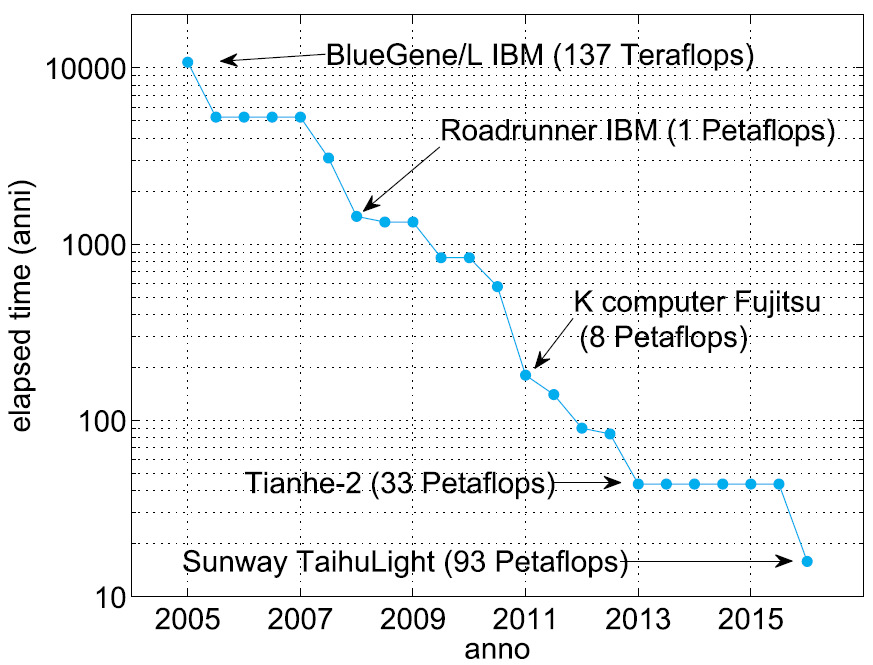
\includegraphics[width=0.72\textwidth]{supercomputer_elapsed_time.png}
\caption{Tempo di calcolo sul miglior supercomputer disponibile per un sistema lineare con $n=24$.}
\end{figure}


\section{Sistemi triangolari}

\subsection{Matrice triangolare inferiore e sostituzioni in avanti}
Sia $L=(\ell_{ij})$ triangolare inferiore, cio\`e
\[
\ell_{ij}=0 \qquad \text{per } i<j.
\]
Allora il sistema $Lx=b$ si risolve sequenzialmente dall'alto verso il basso:
\[
\ell_{11}x_1=b_1
\qquad \Longrightarrow \qquad
x_1=\frac{b_1}{\ell_{11}},
\]
\[
\ell_{21}x_1+\ell_{22}x_2=b_2
\qquad \Longrightarrow \qquad
x_2=\frac{b_2-\ell_{21}x_1}{\ell_{22}},
\]
e in generale
\begin{formulaBox}
\[
 x_i=\frac{b_i-\sum_{j=1}^{i-1}\ell_{ij}x_j}{\ell_{ii}},
 \qquad i=1,\dots,n.
\]
\end{formulaBox}
Questo procedimento prende il nome di \emph{sostituzione in avanti}.

\subsection{Matrice triangolare superiore e sostituzioni all'indietro}
Sia ora $U=(u_{ij})$ triangolare superiore, cio\`e
\[
 u_{ij}=0 \qquad \text{per } i>j.
\]
Il sistema $Ux=b$ si risolve dall'ultima equazione alla prima:
\[
 x_n=\frac{b_n}{u_{nn}},
\]
\begin{formulaBox}
\[
 x_i=\frac{b_i-\sum_{j=i+1}^{n}u_{ij}x_j}{u_{ii}},
 \qquad i=n-1,\dots,1.
\]
\end{formulaBox}
Questo \`e il metodo di \emph{sostituzione all'indietro}.

\begin{figure}[H]
\centering
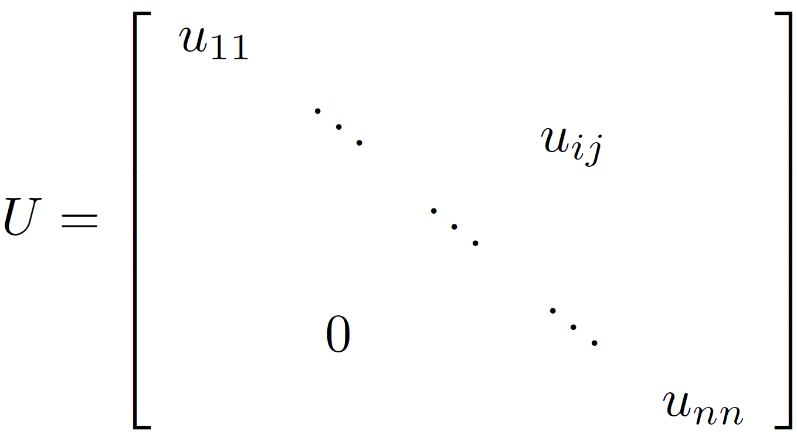
\includegraphics[width=0.62\textwidth]{triangular_upper_scheme.png}
\caption{Matrice triangolare superiore $U$.}
\end{figure}

\subsection{Costo computazionale}
Per le sostituzioni in avanti, per ogni $i$ si effettuano:
\begin{itemize}
  \item $i-1$ moltiplicazioni,
  \item $i-2$ addizioni,
  \item $1$ sottrazione,
  \item $1$ divisione.
\end{itemize}
Quindi il numero totale di operazioni \`e
\[
\sum_{i=1}^n \big((i-1)+(i-2)+1+1\big)
=\sum_{i=1}^n (2i-1)=n^2.
\]
Lo stesso ordine di complessit\`a vale per le sostituzioni all'indietro:
\[
\text{costo} \sim n^2.
\]

\section{Fattorizzazione LU}
Definiamo $A_{p,i}\in\R^{i\times i}$, $i=1,\dots,n$, come la sottomatrice principale ottenuta considerando le prime $i$ righe e le prime $i$ colonne di $A$.

\begin{theorem}[Esistenza e unicit\`a della fattorizzazione LU]
Sia $A\in\R^{n\times n}$. Se
\[
\det(A_{p,i})\neq 0, \qquad i=1,\dots,n-1,
\]
esistono un'unica matrice triangolare inferiore $L$ con diagonale unitaria e un'unica matrice triangolare superiore $U$ tali che
\[
A=LU.
\]
\end{theorem}

Una volta ottenuta la fattorizzazione, il sistema originale si risolve come cascata di due sistemi triangolari:
\[
Ax=b
\quad \Longleftrightarrow \quad
LUx=b
\quad \Longleftrightarrow \quad
\begin{cases}
Ly=b,\\
Ux=y.
\end{cases}
\]

\section{Metodo dell'eliminazione gaussiana (MEG)}
L'idea \`e trasformare progressivamente $A$ in una matrice triangolare superiore annullando gli elementi sotto la diagonale principale.
Introduciamo matrici $A^{(k)}$ e termini noti $b^{(k)}$ a ogni passo, con
\[
A^{(1)}=A,
\qquad
b^{(1)}=b,
\]
\[
A^{(1)}\to A^{(2)}\to\cdots\to A^{(n)}=U,
\qquad
b^{(1)}\to b^{(2)}\to\cdots\to b^{(n)}=y.
\]

Al passo $k$ si annullano gli elementi $a_{ik}^{(k)}$ per $i=k+1,\dots,n$ sottraendo un opportuno multiplo della riga $k$ alle righe successive.
L'algoritmo dettagliato, riportato in un box rosso nei lucidi, \`e il seguente:

% [BOX ROSSO NEI LUCIDI -- NON RICHIESTO ALL'ESAME]
\begin{nonExamBox}
Per $k=1,\dots,n-1$,
\[
\text{per } i=k+1,\dots,n,
\qquad
l_{ik}=\frac{a_{ik}^{(k)}}{a_{kk}^{(k)}},
\]
\[
\text{per } j=k+1,\dots,n,
\qquad
 a_{ij}^{(k+1)}=a_{ij}^{(k)}-l_{ik}a_{kj}^{(k)},
\]
\[
 b_i^{(k+1)}=b_i^{(k)}-l_{ik}b_k^{(k)}.
\]
\end{nonExamBox}
Al termine del MEG si ottengono
\[
A^{(n)}=U,
\qquad
(l_{ij})\leadsto L,
\qquad
b^{(n)}=y.
\]

\subsection{Costo computazionale del MEG}
Per ogni $k=1,\dots,n-1$ si hanno:
\begin{itemize}
  \item $n-k$ operazioni per il calcolo dei moltiplicatori $l_{ik}$;
  \item $2(n-k)^2$ operazioni per l'aggiornamento della matrice;
  \item $2(n-k)$ operazioni per l'aggiornamento del termine noto.
\end{itemize}
Pertanto
\[
\sum_{k=1}^{n-1}\big(2(n-k)^2+3(n-k)\big)
=\sum_{p=1}^{n-1}(2p^2+3p)
\sim \frac{2}{3}n^3.
\]
Quindi il costo complessivo della fattorizzazione LU mediante MEG, seguito dalle sostituzioni all'indietro, \`e dell'ordine
\begin{formulaBox}
\[
\text{costo complessivo }\sim \frac{2}{3}n^3.
\]
\end{formulaBox}

\section{Applicabilit\`a del MEG}
Verificare direttamente le ipotesi del teorema sulla LU richiede il calcolo di $n-1$ determinanti, ed \`e quindi troppo costoso in generale.
Esistono per\`o condizioni sufficienti facili da verificare:
\begin{enumerate}[label=\arabic*)]
  \item \textbf{Dominanza diagonale stretta per righe o per colonne:}
  \[
  |a_{ii}|>\sum_{j\neq i}|a_{ij}|,
  \qquad i=1,\dots,n,
  \]
  oppure analogamente per colonne.
  \item \textbf{Matrice simmetrica definita positiva (SDP):}
  \[
  z\trans Az>0,
  \qquad \forall z\in\R^n,\ z\neq 0.
  \]
\end{enumerate}

\section{Fattorizzazione di Cholesky}
Per matrici simmetriche definite positive vale la fattorizzazione di Cholesky
\[
A=R\trans R,
\]
dove $R$ \`e triangolare superiore.

L'algoritmo dettagliato riportato nei lucidi compare in un box rosso:

% [BOX ROSSO NEI LUCIDI -- NON RICHIESTO ALL'ESAME]
\begin{nonExamBox}
\[
r_{11}=\sqrt{a_{11}},
\qquad
\text{per } j=2,\dots,n,
\]
\[
 r_{ij}=\frac{1}{r_{ii}}\left(a_{ij}-\sum_{k=1}^{i-1} r_{ki}r_{kj}\right),
 \qquad i=1,\dots,j-1,
\]
\[
 r_{jj}=\sqrt{a_{jj}-\sum_{k=1}^{j-1}r_{kj}^2}.
\]
\end{nonExamBox}

Il costo computazionale \`e circa
\[
\frac{1}{3}n^3.
\]

\section{Esempi di eliminazione gaussiana}

\begin{example}[Matrice di Hilbert $3\times 3$]
Sia
\[
A=\begin{bmatrix}
1 & \frac12 & \frac13\\
\frac12 & \frac13 & \frac14\\
\frac13 & \frac14 & \frac15
\end{bmatrix},
\qquad
b=\begin{bmatrix}
\frac{11}{6}\\[2mm]
\frac{13}{12}\\[2mm]
\frac{47}{60}
\end{bmatrix}.
\]
Applicando il MEG si ottiene
\[
A^{(2)}=
\begin{bmatrix}
1 & \frac12 & \frac13\\
0 & \frac1{12} & \frac1{12}\\
0 & \frac1{12} & \frac4{45}
\end{bmatrix},
\qquad
b^{(2)}=
\begin{bmatrix}
\frac{11}{6}\\[2mm]
\frac16\\[2mm]
\frac{31}{180}
\end{bmatrix},
\]
poi
\[
U=A^{(3)}=
\begin{bmatrix}
1 & \frac12 & \frac13\\
0 & \frac1{12} & \frac1{12}\\
0 & 0 & \frac1{180}
\end{bmatrix},
\qquad
y=b^{(3)}=
\begin{bmatrix}
\frac{11}{6}\\[2mm]
\frac16\\[2mm]
\frac1{180}
\end{bmatrix}.
\]
Con sostituzione all'indietro si ricava
\[
 x_3=1,
 \qquad
 x_2=\frac{\frac16-\frac1{12}\cdot 1}{\frac1{12}}=1,
 \qquad
 x_1=\frac{\frac{11}{6}-\frac12\cdot 1-\frac13\cdot 1}{1}=1.
\]
Quindi $x=(1,1,1)\trans$.
\end{example}

\begin{example}[Necessit\`a del pivoting]
Sia
\[
A=\begin{bmatrix}
1 & 1 & 3\\
2 & 2 & 2\\
3 & 6 & 4
\end{bmatrix}.
\]
Applicando il MEG si ottiene al secondo passo
\[
 a_{22}^{(2)}=0,
\]
quindi l'eliminazione si interrompe pur essendo $\det(A)\neq 0$. Il problema nasce dal fatto che
\[
\det(A_{p,2})=0.
\]
Infatti dopo il primo passo si ha
\[
A^{(2)}=
\begin{bmatrix}
1 & 1 & 3\\
0 & 0 & -4\\
0 & 3 & -5
\end{bmatrix}.
\]
Scambiando seconda e terza riga (e analogamente il termine noto) il processo pu\`o proseguire.
\end{example}

\section{Pivoting}
\subsection{Idea generale}
Se al passo $k$ del MEG si ha
\[
a_{kk}^{(k)}=0
\qquad \text{(equivalentemente, } \det(A_{p,k})=0\text{)},
\]
si scambia la riga $k$ con una riga $i>k$ tale che
\[
 a_{ik}^{(k)}\neq 0.
\]
Il pivoting pu\`o essere interpretato come premoltiplicazione per una matrice di permutazione $P$:
\[
PA=LU.
\]
Il sistema si risolve allora come
\[
PAx=Pb
\quad \Longleftrightarrow \quad
LUx=Pb
\quad \Longleftrightarrow \quad
\begin{cases}
Ly=Pb,\\
Ux=y.
\end{cases}
\]

\begin{figure}[H]
\centering
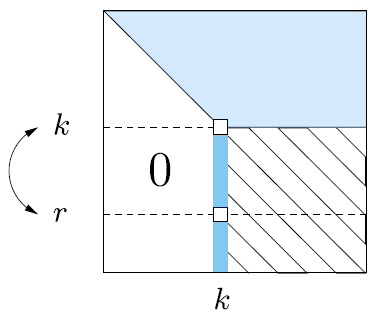
\includegraphics[width=0.42\textwidth]{pivot_row_swap_generic.png}
\caption{Visualizzazione a blocchi dello scambio della riga $k$ con una riga $r>k$ durante il pivoting: il blocco attivo viene riorganizzato in modo da portare in posizione di pivot un coefficiente non nullo.}
\end{figure}

\subsection{Perch\'e il pivoting \`e importante anche in aritmetica finita}
L'operazione che amplifica maggiormente gli errori di arrotondamento \`e la sottrazione.
Nel MEG compare il moltiplicatore
\[
\widehat l_{ik}^{(k)}=\frac{\widehat a_{ik}^{(k)}}{\widehat a_{kk}^{(k)}}
=\frac{a_{ik}^{(k)}+\delta a_{ik}^{(k)}}{a_{kk}^{(k)}+\delta a_{kk}^{(k)}}.
\]
Per ridurre l'effetto degli errori di arrotondamento conviene dunque scegliere un pivot il pi\`u grande possibile in modulo.
Questo porta al \emph{pivoting parziale}:
\begin{formulaBox}
\[
\text{scambio la riga }k\text{ con la riga }\bar r
\quad \text{tale che}\quad
\abs{a_{\bar r k}^{(k)}}=\max_{i\ge k}\abs{a_{ik}^{(k)}}.
\]
\end{formulaBox}

\begin{figure}[H]
\centering
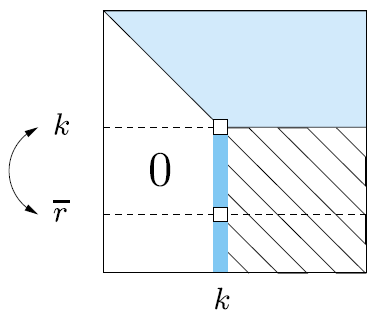
\includegraphics[width=0.38\textwidth]{pivot_partial_choice.png}
\caption{Schema del pivoting parziale: tra le righe $i\ge k$ si sceglie la riga $\bar r$ che massimizza in modulo l'elemento della colonna $k$.}
\end{figure}

\subsection{Pivoting totale}
Nel caso pi\`u generale si possono scambiare anche le colonne, introducendo una seconda matrice di permutazione $Q$:
\[
PAQ=LU.
\]
Allora
\[
Ax=b
\quad \Longleftrightarrow \quad
PAQ\,(Q^{-1}x)=Pb.
\]
Ponendo $x^*=Q^{-1}x$ si risolve
\[
\begin{cases}
Ly=Pb,\\
Ux^*=y,
\end{cases}
\qquad x=Qx^*.
\]

\begin{figure}[H]
\centering
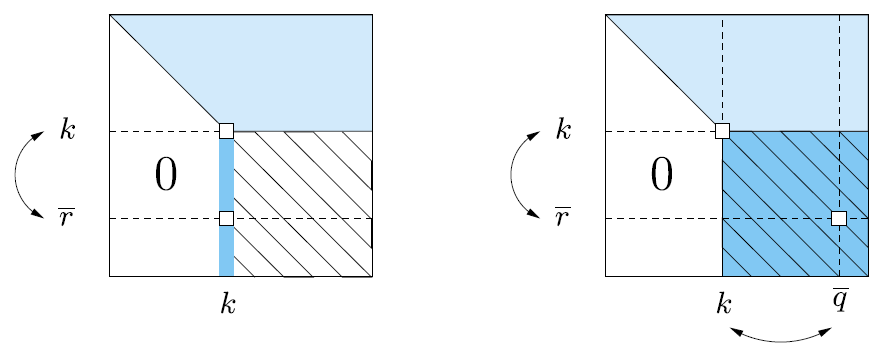
\includegraphics[width=0.82\textwidth]{pivot_partial_total_blocks.png}
\caption{Pivoting parziale e pivoting totale.}
\end{figure}

Il pivoting totale riduce ulteriormente l'errore computazionale, ma non elimina i problemi dovuti al malcondizionamento della matrice.

\section{Errori di arrotondamento e condizionamento}

\subsection{Rappresentazione finita dei numeri}
Nel calcolatore un numero reale $z$ viene memorizzato con un errore di arrotondamento:
\[
\hat z=z+\delta z.
\]
In forma normalizzata si pu\`o scrivere
\[
\hat z=(-1)^s(0.a_1a_2\dots a_t)_\beta\,\beta^{\varrho}
= (-1)^s m\,\beta^{\varrho-t},
\qquad a_1\neq 0,
\]
dove:
\begin{itemize}
  \item $s\in\{0,1\}$ determina il segno,
  \item $\beta$ \`e la base,
  \item $t$ \`e il numero massimo di cifre memorizzate,
  \item $m$ \`e la mantissa.
\end{itemize}
Si ha il bound relativo
\[
\frac{\abs{\delta z}}{\abs z}\le \frac12\beta^{1-t}.
\]
In doppia precisione tipicamente $\beta=2$ e $t=53$, quindi
\[
\frac{\abs{\delta z}}{\abs z}\approx 10^{-16}.
\]

\subsection{Propagazione degli errori nel MEG}
In presenza di aritmetica finita, il sistema effettivamente risolto non \`e esattamente $Ax=b$, ma un sistema perturbato
\[
(A+\delta A)\hat x=b+\delta b.
\]
Sotto l'ipotesi
\[
\norm{\delta A}_2\norm{A^{-1}}_2<1,
\]
vale la stima
\begin{formulaBox}
\[
\frac{\norm{x-\hat x}_2}{\norm{x}_2}
\le
\frac{K_2(A)}{1-K_2(A)\,\norm{\delta A}_2/\norm{A}_2}
\left(
\frac{\norm{\delta A}_2}{\norm{A}_2}+
\frac{\norm{\delta b}_2}{\norm{b}_2}
\right),
\]
\end{formulaBox}
dove
\[
K_2(A)=\norm{A}_2\,\norm{A^{-1}}_2
\]
\`e il numero di condizionamento nella norma euclidea.

\begin{noteBox}
L'errore computazionale dovuto alla propagazione degli arrotondamenti cresce rapidamente quando $K_2(A)$ \`e grande:
matrici malcondizionate sono numericamente delicate.
\end{noteBox}

\begin{figure}[H]
\centering
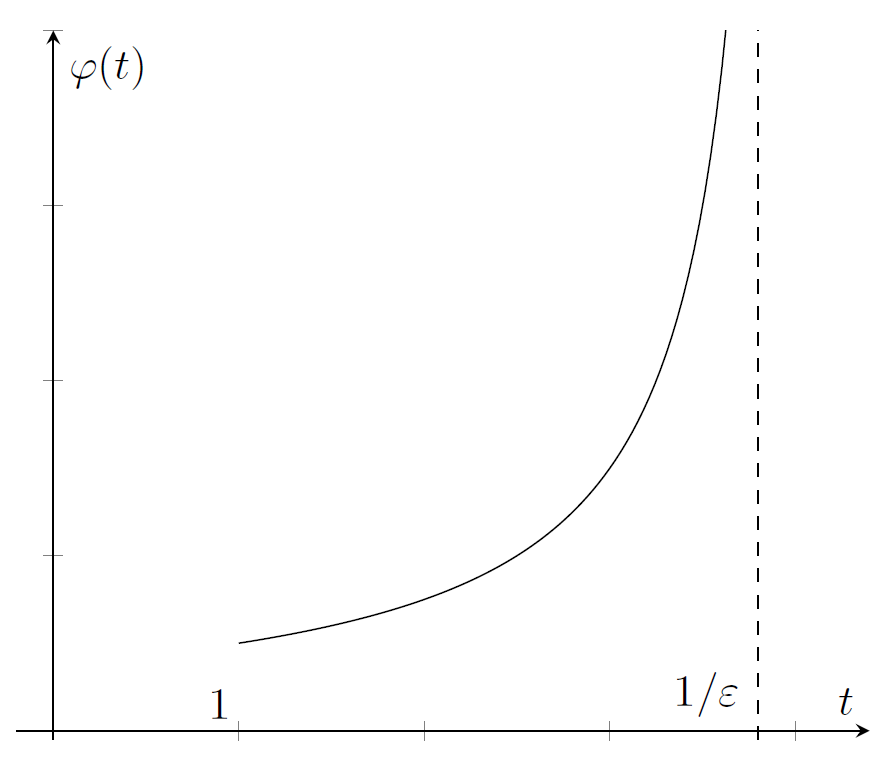
\includegraphics[width=0.72\textwidth]{increment_criterion_gamma.png}
\caption{Propagazione degli errori di arrotondamento nel MEG: per una matrice altamente malcondizionata, la linea continua rappresenta l'errore relativo della soluzione, mentre la linea tratteggiata rappresenta il residuo. Il grafico evidenzia che il residuo pu\`o rimanere piccolo anche quando l'errore relativo \`e molto pi\`u grande.}
\end{figure}

\subsection{Esempio numerico: matrice di Hilbert}
Le matrici di Hilbert costituiscono un esempio classico di matrici fortemente malcondizionate.
All'aumentare della dimensione, piccoli errori di arrotondamento nei dati o nelle operazioni possono produrre errori relativi molto grandi nella soluzione numerica.

\begin{figure}[H]
\centering
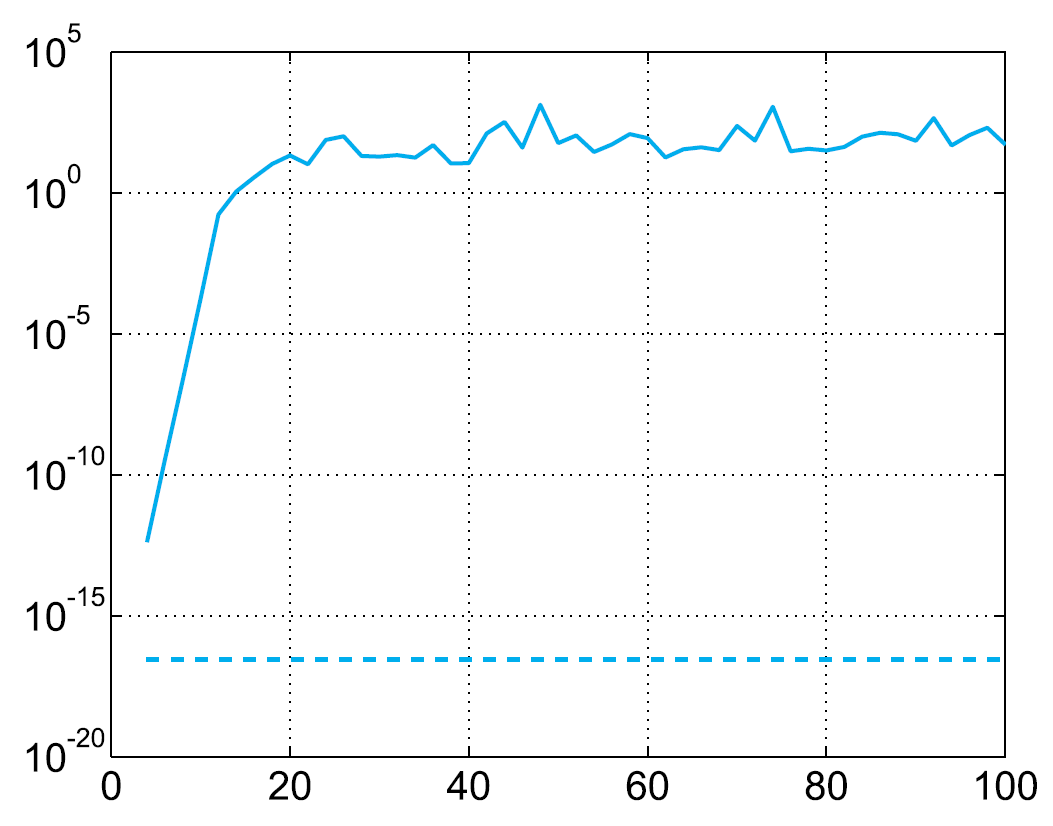
\includegraphics[width=0.76\textwidth]{hilbert_instability.png}
\caption{Matrice di Hilbert altamente malcondizionata: la linea continua rappresenta l'errore relativo della soluzione, mentre la linea tratteggiata rappresenta il residuo. Il grafico mostra che un residuo piccolo non implica necessariamente un errore piccolo quando il problema \`e fortemente malcondizionato.}
\end{figure}

\subsection{Numero di condizionamento per matrici SDP}
Se $A$ \`e simmetrica definita positiva, allora i suoi autovalori sono reali e positivi, e si ottiene
\[
\norm{A}_2=\lambda_{\max}(A),
\qquad
\norm{A^{-1}}_2=\frac1{\lambda_{\min}(A)}.
\]
Di conseguenza,
\begin{formulaBox}
\[
K_2(A)=\frac{\lambda_{\max}(A)}{\lambda_{\min}(A)}.
\]
\end{formulaBox}

\section{Stabilit\`a della soluzione numerica e residuo}
Dato un'approssimazione $\hat x$ della soluzione, definiamo il residuo
\[
r=b-A\hat x.
\]
Sottraendo l'equazione del residuo dal sistema originale si ottiene
\[
r=A(x-\hat x)
\qquad \Longrightarrow \qquad
x-\hat x=A^{-1}r.
\]
Pertanto
\[
\norm{x-\hat x}_2\le \norm{A^{-1}}_2\,\norm r_2.
\]
Poich\'e inoltre
\[
\norm b_2=\norm{Ax}_2\le \norm A_2\,\norm x_2,
\]
segue la stima relativa
\begin{formulaBox}
\[
\frac{\norm{x-\hat x}_2}{\norm{x}_2}
\le K_2(A)\frac{\norm r_2}{\norm b_2}.
\]
\end{formulaBox}
Quindi il residuo \`e un buon indicatore dell'errore solo se il numero di condizionamento \`e piccolo.

\section{Fill-in e matrici sparse}
Il \emph{pattern} di una matrice identifica facilmente la posizione degli elementi diversi da zero.
Una matrice si dice \emph{sparsa} quando il numero di zeri domina fortemente quello degli elementi non nulli; informalmente,
\[
\#\{a_{ij}=0\}\sim n^2,
\qquad
\lim_{n\to\infty}\frac{\#\{a_{ij}\neq 0\}}{n^2}=0.
\]

Il problema del \emph{fill-in} consiste nel fatto che, anche se $A$ \`e sparsa,
i fattori $L$ e $U$ della fattorizzazione LU in generale non lo sono.
Questo rende la LU poco conveniente, dal punto di vista della memoria, per matrici sparse.

Una possibile contromisura \`e il \emph{riordinamento} (reordering), che rinumera righe e colonne per ridurre il fill-in.

Le figure seguenti sono integrative: non introducono nuova teoria, ma aiutano a visualizzare il fenomeno del fill-in e l'effetto del riordinamento nei problemi sparsi.

\begin{figure}[H]
\centering
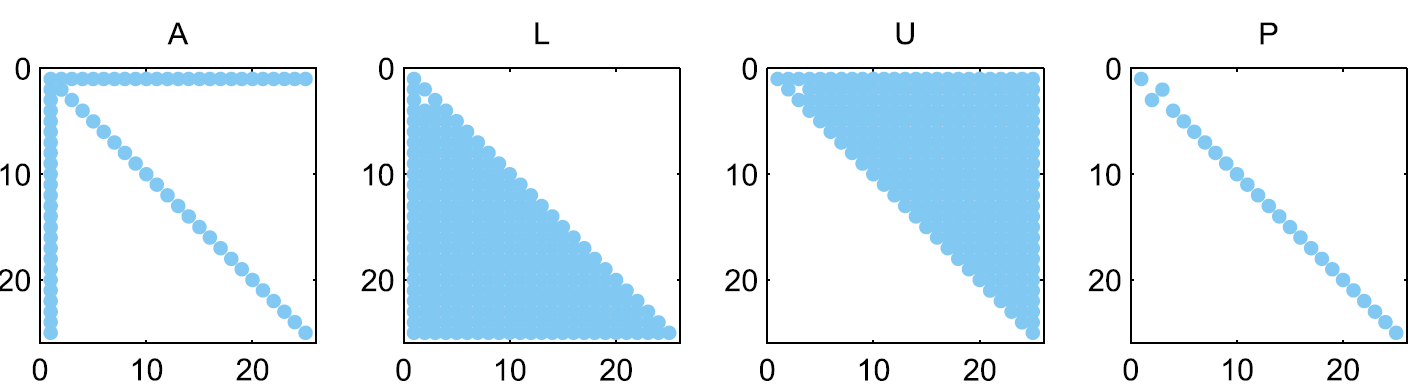
\includegraphics[width=0.92\textwidth]{sparse_A_dense_LU.png}
\caption{Matrice sparsa $A$ e fattori esatti $L$ e $U$: il fill-in pu\`o rendere i fattori quasi pieni.}
\end{figure}

\begin{figure}[H]
\centering
\begin{subfigure}[t]{0.48\textwidth}
  \centering
  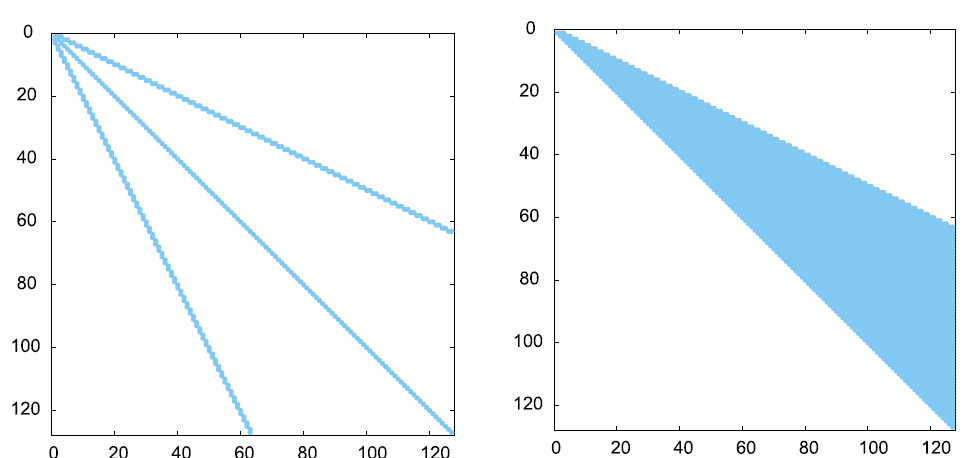
\includegraphics[width=\linewidth]{sparse_vs_dense_upper.png}
  \caption{Matrice A e U prima del riordino.}
\end{subfigure}\hfill
\begin{subfigure}[t]{0.26\textwidth}
  \centering
  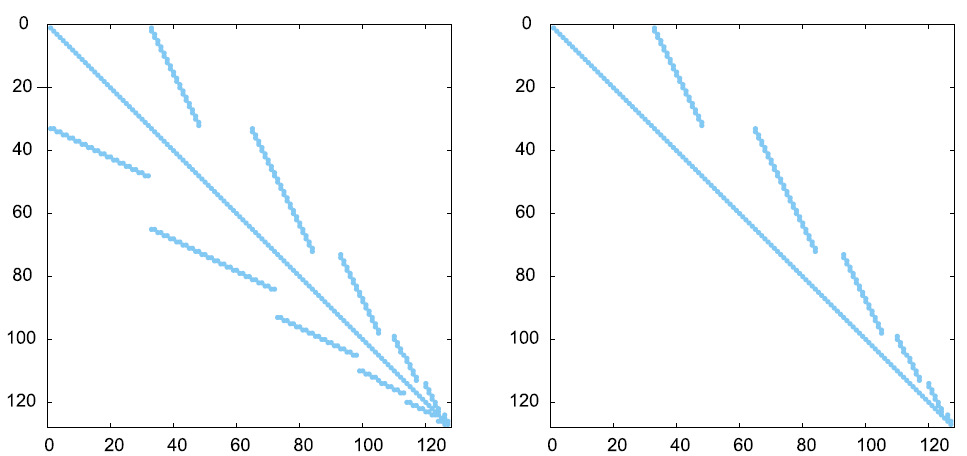
\includegraphics[width=\linewidth]{reordering_effect.png}
  \caption{Matrice A e U dopo il riordino.}
\end{subfigure}
\caption{Per ridurre il fill-in può essere utile eseguire una tecnica di riordinamento, che consiste nel numerare diversamente le righe di A.}
\end{figure}

\chapter{Metodi iterativi per sistemi lineari}

\section{Perch\'e servono i metodi iterativi}
La fattorizzazione LU non \`e sempre conveniente per:
\begin{itemize}
  \item sistemi di grandi dimensioni, perch\'e il costo $\sim \tfrac23 n^3$ pu\`o diventare proibitivo;
  \item matrici sparse, a causa del fill-in.
\end{itemize}
Molti problemi applicativi --- ad esempio discretizzazioni alle differenze finite o agli elementi finiti di equazioni differenziali --- portano proprio a sistemi lineari grandi e sparsi.

\section{Esempio di sistema con matrice sparsa}
Consideriamo il problema differenziale
\[
-u''(x)=f(x),
\qquad x\in(0,1),
\qquad u(0)=u(1)=0.
\]
Discretizzando il dominio e approssimando la derivata seconda si ottiene, per ogni nodo interno $x_j$,
\[
-\frac{u_{j+1}-2u_j+u_{j-1}}{h^2}=f(x_j).
\]
Ne segue il sistema lineare
\[
A u = f_h,
\qquad
A=
\begin{bmatrix}
2 & -1 & 0 & \cdots & 0\\
-1 & 2 & -1 & \ddots & \vdots\\
0 & -1 & 2 & \ddots & 0\\
\vdots & \ddots & \ddots & \ddots & -1\\
0 & \cdots & 0 & -1 & 2
\end{bmatrix},
\]
che \`e tridiagonale e quindi sparso.

\begin{figure}[H]
\centering
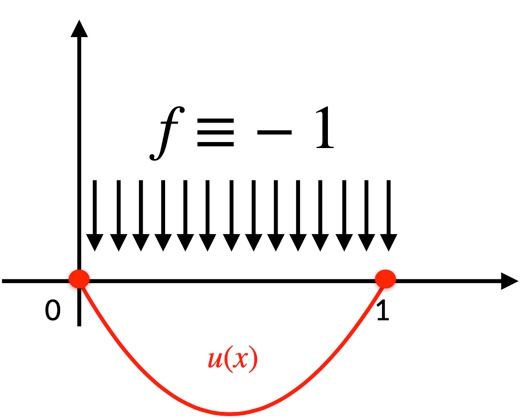
\includegraphics[width=0.56\textwidth]{sparse_string_load.png}
\caption{Interpretazione fisica del problema modello $-u''(x)=f(x)$ con vincoli omogenei agli estremi e forza costante $f\equiv -1$: la discretizzazione porta a un sistema lineare sparso e tridiagonale.}
\end{figure}

\section{Definizione di metodo iterativo}
Un metodo iterativo genera una successione di vettori
\[
x^{(0)},x^{(1)},x^{(2)},\dots
\]
a partire da un vettore iniziale $x^{(0)}$.
Affinch\'e il metodo abbia senso, dev'essere soddisfatta la convergenza:
\[
\lim_{k\to\infty}x^{(k)}=x,
\]
dove $x$ \`e la soluzione esatta del sistema.

Anche in aritmetica esatta un metodo iterativo \`e inevitabilmente affetto da errore numerico, perch\'e in pratica il processo viene arrestato dopo un numero finito di iterazioni.

\section{Metodo di Jacobi}
Dalla $i$-esima equazione del sistema
\[
\sum_{j=1}^n a_{ij}x_j=b_i
\]
si ricava formalmente
\[
 x_i=\frac{b_i-\sum_{j\neq i}a_{ij}x_j}{a_{ii}}.
\]
Il metodo di Jacobi aggiorna $x_i$ usando i valori del passo precedente:
\begin{formulaBox}
\[
 x_i^{(k+1)}=
 \frac{b_i-\sum_{j\neq i}a_{ij}x_j^{(k)}}{a_{ii}},
 \qquad i=1,\dots,n.
\]
\end{formulaBox}
Ogni iterazione costa $\sim n^2$ operazioni in generale, ma soltanto $\sim n$ se la matrice \`e sparsa.
Un vantaggio importante \`e che le componenti $x_i^{(k+1)}$ possono essere calcolate in parallelo.

\section{Metodo di Gauss--Seidel}
Nel metodo di Gauss--Seidel, quando si aggiorna la componente $i$, i valori con indice minore sono gi\`a stati aggiornati al passo corrente. Quindi
\begin{formulaBox}
\[
 x_i^{(k+1)}=
 \frac{b_i-\sum_{j<i}a_{ij}x_j^{(k+1)}-\sum_{j>i}a_{ij}x_j^{(k)}}{a_{ii}},
 \qquad i=1,\dots,n.
\]
\end{formulaBox}
I costi computazionali sono comparabili a quelli di Jacobi, ma qui il calcolo non \`e naturalmente parallelo.

\section{Metodi iterativi lineari}
In generale consideriamo metodi del tipo
\[
 x^{(k+1)}=Bx^{(k)}+f,
\]
dove $B\in\R^{n\times n}$ \`e la \emph{matrice di iterazione} e $f\in\R^n$ identifica il metodo.

\subsection{Consistenza}
Se il metodo applicato alla soluzione esatta non deve modificarla, allora
\[
 x=Bx+f.
\]
Poich\'e $Ax=b$, segue
\[
 f=(I-B)x=(I-B)A^{-1}b.
\]
Questa \`e una condizione necessaria, ma non sufficiente, per la convergenza.

\subsection{Convergenza e raggio spettrale}
Definiamo l'errore
\[
 e^{(k)}=x-x^{(k)}.
\]
Dalla consistenza si ottiene
\[
 e^{(k+1)}=Be^{(k)},
\qquad
\norm{e^{(k+1)}}\le \norm B\,\norm{e^{(k)}}.
\]
Applicando ricorsivamente la disuguaglianza,
\[
\norm{e^{(k+1)}}\le \norm B^{k+1}\,\norm{e^{(0)}}.
\]
Quindi una condizione sufficiente di convergenza \`e
\[
\norm B<1.
\]

Definiamo il raggio spettrale di $B$ come
\[
\rho(B)=\max_j \abs{\lambda_j(B)}.
\]
Vale il criterio fondamentale:
\begin{theorem}
Il metodo iterativo lineare converge se e solo se
\[
\rho(B)<1.
\]
\end{theorem}
Inoltre, per ogni norma matriciale indotta,
\[
\rho(B)\le \norm B.
\]

\section{Convergenza di Jacobi e Gauss--Seidel}
Scriviamo
\[
A=D-E-F,
\]
dove $D$ \`e la diagonale di $A$, $-E$ la parte triangolare inferiore e $-F$ la parte triangolare superiore.

\begin{figure}[H]
\centering
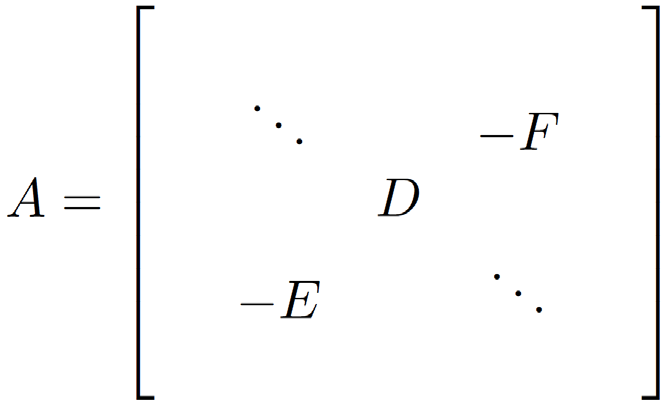
\includegraphics[width=0.56\textwidth]{splitting_DEF.png}
\caption{Schema della decomposizione $A=D-E-F$ usata per scrivere in forma compatta i metodi di Jacobi e di Gauss--Seidel.}
\end{figure}

Per Jacobi:
\[
Dx^{(k+1)}=(E+F)x^{(k)}+b,
\qquad
B_J=D^{-1}(E+F)=D^{-1}(D-A)=I-D^{-1}A.
\]
Per Gauss--Seidel:
\[
(D-E)x^{(k+1)}=Fx^{(k)}+b,
\qquad
B_{GS}=(D-E)^{-1}F.
\]
Entrambi i metodi sono consistenti perch\'e $D-E-F=A$ e $Ax=b$.

Risultati utili di convergenza:
\begin{itemize}
  \item Se $A$ \`e strettamente dominante diagonale per righe, allora Jacobi e Gauss--Seidel convergono.
  \item Se $A$ \`e simmetrica definita positiva, allora Gauss--Seidel converge.
  \item Se $A$ \`e tridiagonale, Jacobi e Gauss--Seidel o convergono entrambi o non convergono entrambi; se convergono, Gauss--Seidel \`e pi\`u veloce.
\end{itemize}

% [BOX ROSSO NEI LUCIDI -- NON RICHIESTO ALL'ESAME]
\begin{nonExamBox}
\textbf{Dimostrazione (caso Jacobi in norma $\|\cdot\|_1$).}
Si ha
\[
-D^{-1}A=
\begin{bmatrix}
-1 &        &        & -a_{1j}/a_{11} \\
   & \ddots &        & \vdots \\
-a_{ij}/a_{ii} & & \ddots & \\
   &        &        & -1
\end{bmatrix},
\qquad
B_J=I-D^{-1}A.
\]
Quindi $B_J$ ha diagonale nulla e coefficienti fuori diagonale pari a $-a_{ij}/a_{ii}$.
Prendendo la norma matriciale indotta
\[
\|C\|_1=\max_i \sum_j |c_{ij}|,
\]
si ottiene
\[
\|B_J\|_1=\max_i \sum_j |(B_J)_{ij}|
       =\max_i \sum_{j\neq i}\left|\frac{a_{ij}}{a_{ii}}\right|.
\]
Se $A$ \`e strettamente dominante diagonale per righe, allora
\[
\sum_{j\neq i}\left|\frac{a_{ij}}{a_{ii}}\right|<1
\qquad \forall i,
\]
e dunque $\|B_J\|_1<1$, da cui segue la convergenza.
\end{nonExamBox}

\section{Metodo di Richardson stazionario}
Il metodo di Richardson stazionario \`e definito da
\begin{formulaBox}
\[
 x^{(k+1)}=x^{(k)}+\alpha\bigl(b-Ax^{(k)}\bigr),
\]
\end{formulaBox}
dove $\alpha\in\R$ \`e un parametro fissato e
\[
 r^{(k)}=b-Ax^{(k)}
\]
\`e il residuo al passo $k$.

Equivalentemente,
\[
 x^{(k+1)}=(I-\alpha A)x^{(k)}+\alpha b,
\]
quindi
\[
 B_\alpha=I-\alpha A,
\qquad
f=\alpha b.
\]

\subsection{Convergenza per matrici SPD}
Supponiamo $A$ simmetrica definita positiva. Se
\[
\lambda_{\max}(A)=\lambda_1(A)\ge \cdots \ge \lambda_n(A)=\lambda_{\min}(A)>0,
\]
allora il metodo converge se e solo se
\begin{formulaBox}
\[
0<\alpha<\frac{2}{\lambda_{\max}(A)}.
\]
\end{formulaBox}


% [BOX ROSSO NEI LUCIDI -- NON RICHIESTO ALL'ESAME]
\begin{nonExamBox}
\textbf{Dimostrazione.}
Siano $\mu_i$ gli autovalori di $B_\alpha$. Poich\'e
\[
B_\alpha=I-\alpha A,
\]
si ha
\[
\mu_i=1-\alpha\lambda_i(A), \qquad i=1,\dots,n.
\]
La convergenza equivale a $\rho(B_\alpha)<1$, cio\`e
\[
|1-\alpha\lambda_i(A)|<1, \qquad i=1,\dots,n.
\]
Equivalentemente,
\[
-1<1-\alpha\lambda_i(A)<1,
\]
da cui
\[
0<\alpha\lambda_i(A)<2, \qquad i=1,\dots,n.
\]
La prima disuguaglianza \`e verificata se $\alpha>0$, mentre la seconda richiede
\[
\alpha<\frac{2}{\lambda_i(A)}, \qquad i=1,\dots,n.
\]
Essendo $\lambda_{\max}(A)$ il massimo autovalore, basta imporre
\[
0<\alpha<\frac{2}{\lambda_{\max}(A)}.
\]
\end{nonExamBox}

\subsection{Scelta del parametro ottimale}
Vogliamo scegliere $\alpha$ in modo da massimizzare la velocit\`a di convergenza, cio\`e minimizzare il raggio spettrale di $B_\alpha$.
Usando la norma indotta da $A$,
\[
\norm z_A=\sqrt{z\trans Az},
\]
si cerca
\[
\alpha_{opt}=\argmin_{0<\alpha<2/\lambda_{\max}(A)}\max_i\abs{1-\alpha\lambda_i(A)}.
\]
Dal confronto tra i grafici delle quantit\`a $\abs{1-\alpha\lambda_i(A)}$ si ricava
\begin{formulaBox}
\[
\alpha_{opt}=\frac{2}{\lambda_{\min}(A)+\lambda_{\max}(A)}.
\]
\end{formulaBox}
In corrispondenza del parametro ottimale,
\[
\rho_{opt}=\rho(B_{\alpha_{opt}})
=\frac{\lambda_{\max}(A)-\lambda_{\min}(A)}{\lambda_{\max}(A)+\lambda_{\min}(A)}.
\]
Per matrici SPD, usando
\[
K(A)=\frac{\lambda_{\max}(A)}{\lambda_{\min}(A)},
\]
si ottiene la forma equivalente
\begin{formulaBox}
\[
\rho_{opt}=\frac{K(A)-1}{K(A)+1}.
\]
\end{formulaBox}

\begin{figure}[H]
\centering
\begin{subfigure}[t]{0.48\textwidth}
  \centering
  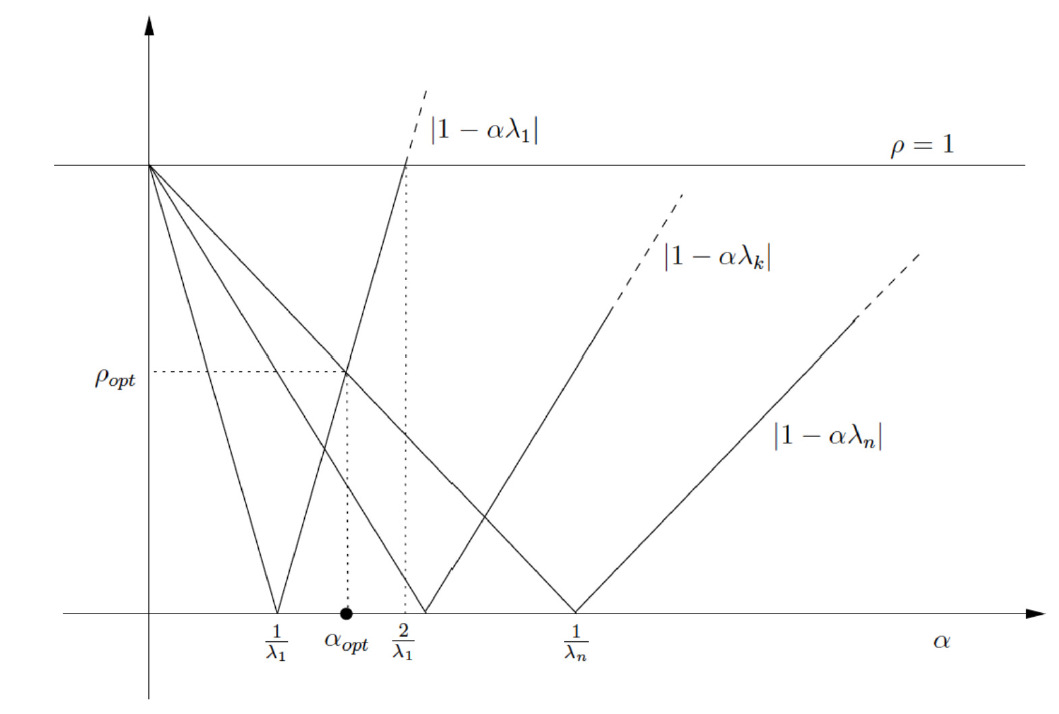
\includegraphics[width=\linewidth]{richardson_alpha_opt_plain.png}
  \caption{Andamento delle quantità $\lvert 1-\alpha\lambda_i(A)\rvert$ al variare di $\alpha$.}
\end{subfigure}\hfill
\begin{subfigure}[t]{0.48\textwidth}
  \centering
  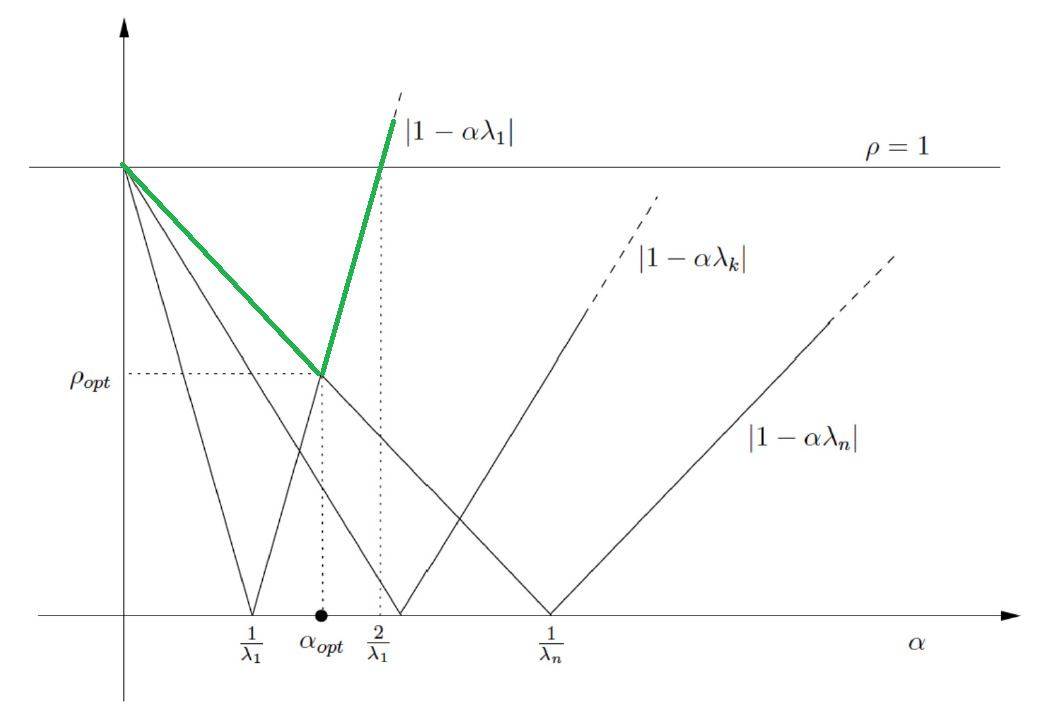
\includegraphics[width=\linewidth]{richardson_alpha_opt_highlight.png}
  \caption{Il parametro ottimale si ottiene nel punto in cui il massimo di tali quantità è minimo.}
\end{subfigure}
\caption{Interpretazione grafica della scelta di $\alpha_{opt}$ nel metodo di Richardson stazionario per matrici SPD.}
\end{figure}

\section{Precondizionamento}
Sia $P$ una matrice invertibile e, nel contesto dei lucidi, simmetrica definita positiva. Il sistema originario \`e equivalente a
\[
P^{-1}Ax=P^{-1}b.
\]
Applicando Richardson al sistema precondizionato si ottiene
\[
 x^{(k+1)}=x^{(k)}+\alpha P^{-1}(b-Ax^{(k)})=x^{(k)}+\alpha P^{-1}r^{(k)}.
\]
I risultati di convergenza del caso non precondizionato si trasferiscono sostituendo $A$ con $P^{-1}A$:
\[
0<\alpha<\frac{2}{\lambda_{\max}(P^{-1}A)},
\qquad
\alpha_{opt}=\frac{2}{\lambda_{\min}(P^{-1}A)+\lambda_{\max}(P^{-1}A)},
\]
\[
\rho_{opt}=\frac{K(P^{-1}A)-1}{K(P^{-1}A)+1}.
\]

\begin{noteBox}
Se $K(P^{-1}A)\ll K(A)$, il numero di iterazioni richiesto diminuisce notevolmente.
Tuttavia il tempo totale di calcolo dipende anche dal costo della singola iterazione:
\[
\text{CPU time}=\#Iter\times C.
\]
\end{noteBox}

Definendo il residuo precondizionato
\[
 z^{(k)}=P^{-1}r^{(k)},
\]
un algoritmo pratico \`e:
\[
 r^{(k)}=b-Ax^{(k)},
\qquad
 Pz^{(k)}=r^{(k)},
\qquad
 x^{(k+1)}=x^{(k)}+\alpha_{opt} z^{(k)}.
\]

\subsection{Come scegliere il precondizionatore}
Un buon precondizionatore deve soddisfare due requisiti:
\begin{enumerate}[label=\arabic*)]
  \item ridurre sensibilmente il condizionamento, cio\`e $K(P^{-1}A)\ll K(A)$;
  \item rendere facile la risoluzione dei sistemi lineari in $P$.
\end{enumerate}
Per questo motivo $P$ viene spesso scelto diagonale, triangolare oppure come prodotto di matrici con struttura semplice.

\subsection{Esempio: fattorizzazione LU inesatta (ILU)}
Per sistemi sparsi \`e utile costruire un precondizionatore del tipo
\[
P_{ILU}=\widetilde L\,\widetilde U,
\]
dove $\widetilde L$ e $\widetilde U$ sono ottenuti eseguendo un'eliminazione gaussiana incompleta imponendo a priori
\[
\widetilde \ell_{ij}=0,
\qquad
\widetilde u_{ij}=0
\qquad \text{se } a_{ij}=0.
\]
Cos\`i i fattori incompleti mantengono la stessa sparsity di $A$ e possono essere usati come precondizionatori: non coincidono con la LU esatta, ma contengono informazione utile su $A$ e restano economici da usare.

\begin{figure}[H]
\centering
\begin{subfigure}[t]{0.58\textwidth}
  \centering
  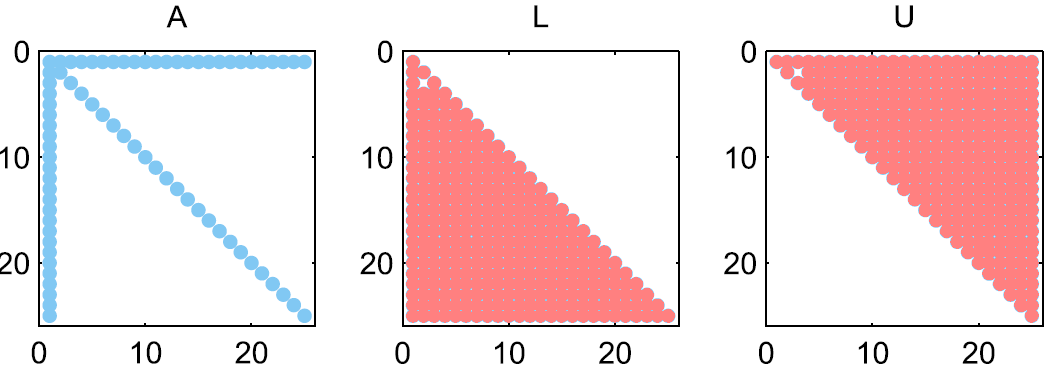
\includegraphics[width=\linewidth]{exact_sparse_ALU.png}
  \caption{Matrice sparsa $A$ e fattori esatti $L$, $U$.}
\end{subfigure}\hfill
\begin{subfigure}[t]{0.34\textwidth}
  \centering
  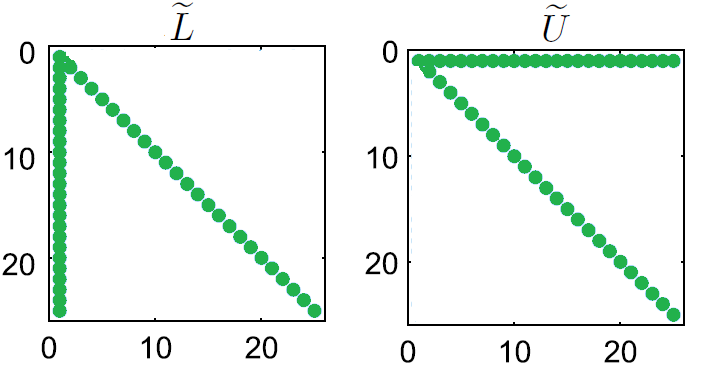
\includegraphics[width=\linewidth]{ilu_sparse_factors.png}
  \caption{Fattori incompleti $\widetilde L$, $\widetilde U$.}
\end{subfigure}
\caption{Fattorizzazione LU esatta e fattorizzazione LU inesatta (ILU).}
\end{figure}

\section{Metodo del gradiente (steepest descent)}
Supponiamo $A$ simmetrica definita positiva. Introduciamo la funzione energia
\[
\Phi(y)=\frac12 y\trans Ay-y\trans b.
\]
Poich\'e
\[
\nabla \Phi(y)=Ay-b,
\]
il punto di minimo di $\Phi$ coincide con la soluzione di $Ax=b$.

\begin{figure}[H]
\centering
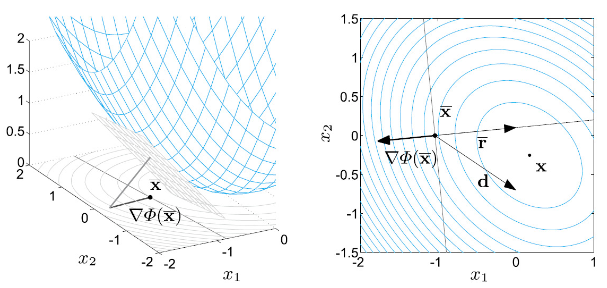
\includegraphics[width=0.78\textwidth]{gradient_geometry.png}
\caption{Interpretazione geometrica del metodo del gradiente: ci si muove nella direzione di massima decrescita dell'energia, cioè lungo $-\nabla\Phi(x^{(k)})$.}
\end{figure}

La direzione di massima decrescita dell'energia nel punto $x^{(k)}$ \`e $-\nabla\Phi(x^{(k)})$, cio\`e il residuo
\[
-\nabla\Phi(x^{(k)})=-Ax^{(k)}+b=r^{(k)}.
\]
Il metodo del gradiente assume quindi l'aggiornamento
\begin{formulaBox}
\[
 x^{(k+1)}=x^{(k)}-\alpha_k\nabla\Phi(x^{(k)})=x^{(k)}+\alpha_k r^{(k)}.
\]
\end{formulaBox}

\subsection{Scelta dinamica del parametro}
Si sceglie $\alpha_k$ minimizzando l'energia lungo la direzione del residuo. Impostando
\[
\frac{d\Phi(x^{(k+1)})}{d\alpha_k}=0,
\]
si ottiene il valore ottimale seguente:
\begin{formulaBox}
\[
\alpha_k=\frac{(r^{(k)})\trans r^{(k)}}{(r^{(k)})\trans Ar^{(k)}}.
\]
\end{formulaBox}

% [BOX ROSSO NEI LUCIDI -- NON RICHIESTO ALL'ESAME]
\begin{nonExamBox}
\textbf{Calcolo del parametro dinamico.}
Poich\'e
\[
x^{(k+1)}=x^{(k)}+\alpha_k r^{(k)},
\]
si ha
\[
\Phi(x^{(k+1)})
=\frac12\bigl(x^{(k)}+\alpha_k r^{(k)}\bigr)\trans A\bigl(x^{(k)}+\alpha_k r^{(k)}\bigr)
-\bigl(x^{(k)}+\alpha_k r^{(k)}\bigr)\trans b.
\]
Sviluppando,
\[
\Phi(x^{(k+1)})
=\frac12 (x^{(k)})\trans Ax^{(k)}
+\frac12\alpha_k (x^{(k)})\trans Ar^{(k)}
+\frac12\alpha_k (r^{(k)})\trans Ax^{(k)}
+\frac12\alpha_k^2 (r^{(k)})\trans Ar^{(k)}
-(x^{(k)})\trans b-\alpha_k (r^{(k)})\trans b.
\]
Essendo $A=A\trans$, vale
\[
(x^{(k)})\trans Ar^{(k)}=(r^{(k)})\trans Ax^{(k)},
\]
e quindi
\[
0=\frac{d\Phi(x^{(k+1)})}{d\alpha_k}
=(r^{(k)})\trans Ax^{(k)}+\alpha_k (r^{(k)})\trans Ar^{(k)}-(r^{(k)})\trans b.
\]
Poich\'e $r^{(k)}=b-Ax^{(k)}$, si ottiene
\[
(r^{(k)})\trans Ax^{(k)}-(r^{(k)})\trans b=-(r^{(k)})\trans r^{(k)},
\]
da cui segue
\[
\alpha_k=\frac{(r^{(k)})\trans r^{(k)}}{(r^{(k)})\trans Ar^{(k)}}.
\]
\end{nonExamBox}

Il metodo del gradiente pu\`o dunque essere visto come un metodo di Richardson con parametro dinamico.

\section{Metodo del gradiente coniugato (GC)}
La velocit\`a di convergenza del gradiente resta legata al condizionamento, come per Richardson ottimale.
Per migliorare l'esplorazione di $\R^n$, si introducono direzioni $d^{(k)}$ tra loro coniugate rispetto ad $A$:
\[
(d^{(k)},d^{(j)})_A=(d^{(k)})\trans A d^{(j)}=0,
\qquad j<k.
\]

\subsection{Algoritmo}
Dato $x^{(0)}$, si pone
\[
 r^{(0)}=b-Ax^{(0)},
 \qquad
 d^{(0)}=r^{(0)}.
\]
Per $k=0,1,\dots$ si esegue il seguente schema ricorsivo.

% [BOX ROSSO NEI LUCIDI -- NON RICHIESTO ALL'ESAME]
\begin{nonExamBox}
\[
\alpha_k=\frac{(d^{(k)})\trans r^{(k)}}{(d^{(k)})\trans A d^{(k)}},
\]
\[
 x^{(k+1)}=x^{(k)}+\alpha_k d^{(k)},
\qquad
 r^{(k+1)}=r^{(k)}-\alpha_k A d^{(k)},
\]
\[
 \beta_k=\frac{(Ad^{(k)})\trans r^{(k+1)}}{(Ad^{(k)})\trans d^{(k)}},
\qquad
 d^{(k+1)}=r^{(k+1)}-\beta_k d^{(k)}.
\]
\end{nonExamBox}
Il costo della singola iterazione \`e paragonabile a quello dei metodi di Richardson e del gradiente, ma il metodo \`e molto pi\`u efficace per matrici sparse SPD.

\begin{theorem}
In aritmetica esatta, il metodo del gradiente coniugato converge alla soluzione esatta in al pi\`u $n$ iterazioni.
\end{theorem}
In pratica, gli errori di arrotondamento impediscono il raggiungimento esatto in $n$ passi, ma il risultato spiega l'elevata velocit\`a di convergenza osservata.

\begin{figure}[H]
\centering
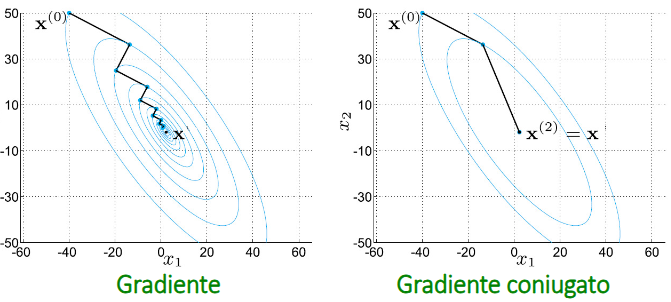
\includegraphics[width=0.82\textwidth]{gradient_vs_cg_path.png}
\caption{Gradiente e gradiente coniugato.}
\end{figure}

\subsection{Stima di convergenza}
Per matrici SPD si ha la stima
\begin{formulaBox}
\[
\norm{e^{(k)}}_A
\le
\frac{2c^k}{1+c^{2k}}\norm{e^{(0)}}_A,
\qquad
c=\frac{\sqrt{K(A)}-1}{\sqrt{K(A)}+1}.
\]
\end{formulaBox}
Per confronto, il metodo del gradiente soddisfa invece una stima del tipo
\[
\norm{e^{(k)}}_A\le
\left(\frac{K(A)-1}{K(A)+1}\right)^k \norm{e^{(0)}}_A,
\]
quindi, per matrici SPD, il gradiente coniugato converge pi\`u rapidamente.

\begin{figure}[H]
\centering
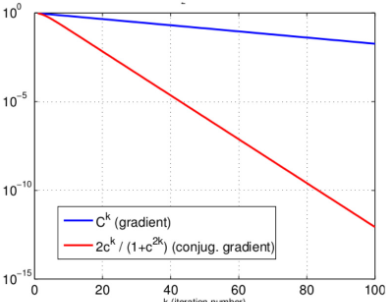
\includegraphics[width=0.50\textwidth]{gradient_vs_cg_bound.png}
\caption{Confronto tra le stime teoriche di convergenza del metodo del gradiente e del gradiente coniugato.}
\end{figure}

\section{Gradiente coniugato precondizionato}
Nel caso precondizionato il comportamento dell'errore si ottiene sostituendo $A$ con $P^{-1}A$ nelle stime precedenti. In particolare,
\[
\norm{e^{(k)}}_A
\le
\frac{2c^k}{1+c^{2k}}\norm{e^{(0)}}_A,
\qquad
c=\frac{\sqrt{K(P^{-1}A)}-1}{\sqrt{K(P^{-1}A)}+1}.
\]
Se il precondizionatore \`e ben scelto, allora
\[
\frac{\sqrt{K(P^{-1}A)}-1}{\sqrt{K(P^{-1}A)}+1}
<
\frac{\sqrt{K(A)}-1}{\sqrt{K(A)}+1},
\]
per cui l'errore si riduce pi\`u velocemente rispetto al caso non precondizionato.

\section{Criteri di arresto}
Poich\'e l'errore esatto
\[
 e^{(k)}=x-x^{(k)}
\]
non \`e calcolabile senza conoscere $x$, si devono usare criteri pratici per arrestare il processo iterativo.

\subsection{Criterio sul residuo}
Abbiamo visto che
\[
\frac{\norm{x-x^{(k)}}}{\norm x}
\le K(A)\frac{\norm{r^{(k)}}}{\norm b}.
\]
Questo suggerisce il test
\begin{formulaBox}
\[
\frac{\norm{r^{(k)}}}{\norm b}\le \varepsilon.
\]
\end{formulaBox}
Per metodi precondizionati, usando $z^{(k)}=P^{-1}r^{(k)}$, si impiega spesso
\[
\frac{\norm{z^{(k)}}}{\norm b}\le \varepsilon,
\]
che \`e affidabile se $K(P^{-1}A)$ \`e piccolo.


\begin{figure}[H]
\centering
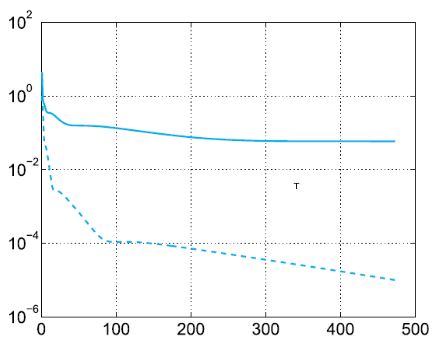
\includegraphics[width=0.52\textwidth]{residual_stopping_semilog_correct.png}
\caption{Andamento, al variare di $k$, del residuo relativo (linea tratteggiata) e dell'errore $\norm{x-x^{(k)}}/\norm{x}$ (linea continua) per il metodo di Gauss-Seidel applicato a un sistema con matrice di Hilbert. Il grafico mostra che il residuo pu\`o risultare molto pi\`u piccolo dell'errore effettivo.}
\end{figure}


\subsection{Criterio sull'incremento}
Definiamo l'incremento
\[
\delta^{(k)}=x^{(k+1)}-x^{(k)}.
\]
Per un metodo lineare con matrice di iterazione $B$ vale la relazione
\[
\norm{e^{(k)}}\le \frac{1}{1-\rho(B)}\norm{\delta^{(k)}}.
\]
Questo porta al criterio
\begin{formulaBox}
\[
\norm{\delta^{(k)}}\le \varepsilon.
\]
\end{formulaBox}
Il criterio sull'incremento \`e buono quando $\rho(B)$ \`e piccolo, mentre pu\`o risultare poco affidabile se $\rho(B)$ \`e vicino a $1$.



\chapter{Ricerca di radici di funzioni non lineari}

\section{Formulazione del problema}
Dato un intervallo $(a,b)$ e una funzione
\[
 f:(a,b)\to\R,
\]
si vuole determinare un punto $\alpha\in(a,b)$ tale che
\[
 f(\alpha)=0.
\]
Il punto $\alpha$ si dice \emph{zero} di $f$ oppure \emph{radice} dell'equazione $f(x)=0$.
In generale il problema non \`e banale perch\'e la funzione pu\`o essere non lineare.


\begin{figure}[H]
\centering
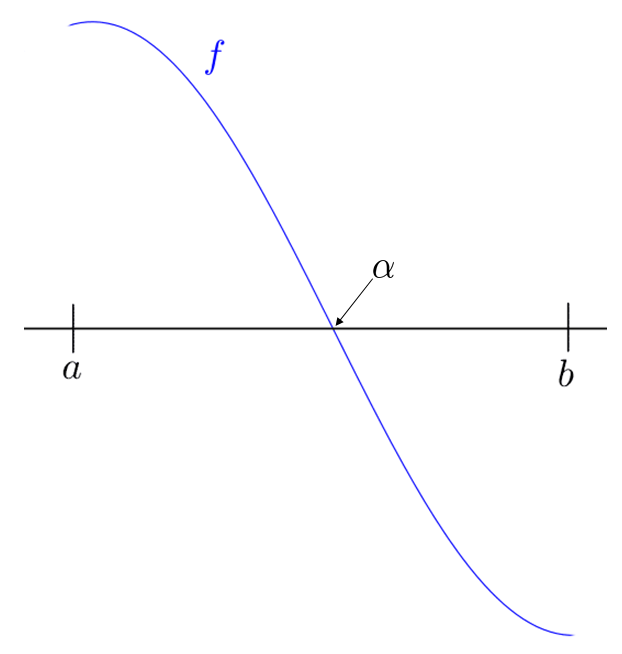
\includegraphics[width=0.46\textwidth]{nonlinear_root_intro.png}
\caption{Ricerca di una radice $\alpha\in(a,b)$ di una funzione non lineare.}
\end{figure}

\subsection{Esempio: equazione di stato di un gas}
Per un gas a temperatura $T$ e pressione $p$, il volume $V$ occupato pu\`o essere determinato mediante l'equazione di stato
\[
\left[p+a\left(\frac{N}{V}\right)^2\right](V-Nb)=kNT,
\]
dove $a$ e $b$ sono coefficienti caratteristici del gas, $N$ \`e il numero di molecole contenute in $V$ e $k$ \`e la costante di Boltzmann.
Il problema si riconduce quindi alla ricerca degli zeri della funzione
\[
 f(V)=\left[p+a\left(\frac{N}{V}\right)^2\right](V-Nb)-kNT.
\]

\section{Metodi iterativi locali}
Un metodo iterativo costruisce una successione
\[
 x^{(0)},x^{(1)},x^{(2)},\dots,x^{(k)},\dots
\]
a partire da un dato iniziale $x^{(0)}$, con l'obiettivo di ottenere
\[
 \lim_{k\to\infty}x^{(k)}=\alpha.
\]
I metodi presentati in questi lucidi sono \emph{locali}: la convergenza \`e garantita solo se il dato iniziale \`e sufficientemente vicino alla radice.

\subsection{Metodo di Newton}
Approssimando $f$ con la tangente nel punto $x^{(k)}$, si ottiene
\begin{formulaBox}
\[
 x^{(k+1)}=x^{(k)}-\frac{f\bigl(x^{(k)}\bigr)}{f'\bigl(x^{(k)}\bigr)},
 \qquad k\ge 0.
\]
\end{formulaBox}
Il metodo richiede la conoscenza della derivata prima.

\begin{figure}[H]
\centering
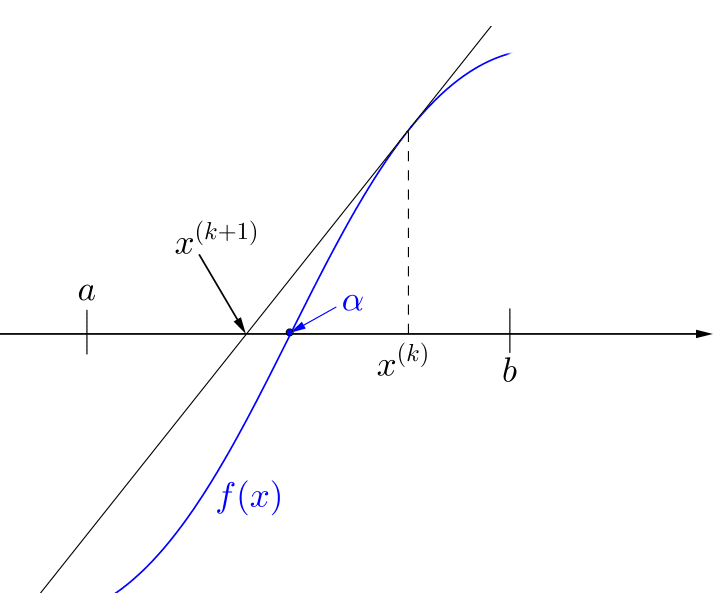
\includegraphics[width=0.60\textwidth]{newton_geometry.png}
\caption{Interpretazione geometrica del metodo di Newton: la nuova iterata si ottiene intersecando con l'asse $x$ la tangente al grafico di $f$ nel punto $x^{(k)}$.}
\end{figure}

\subsection{Metodo delle corde}
Si sostituisce la derivata con la pendenza costante della corda che unisce gli estremi dell'intervallo:
\begin{formulaBox}
\[
 x^{(k+1)}=x^{(k)}-\frac{f\bigl(x^{(k)}\bigr)}{q},
 \qquad
 q=\frac{f(b)-f(a)}{b-a}\neq 0.
\]
\end{formulaBox}
Il metodo evita il calcolo di $f'$ ma usa un coefficiente fisso $q$.

\begin{figure}[H]
\centering
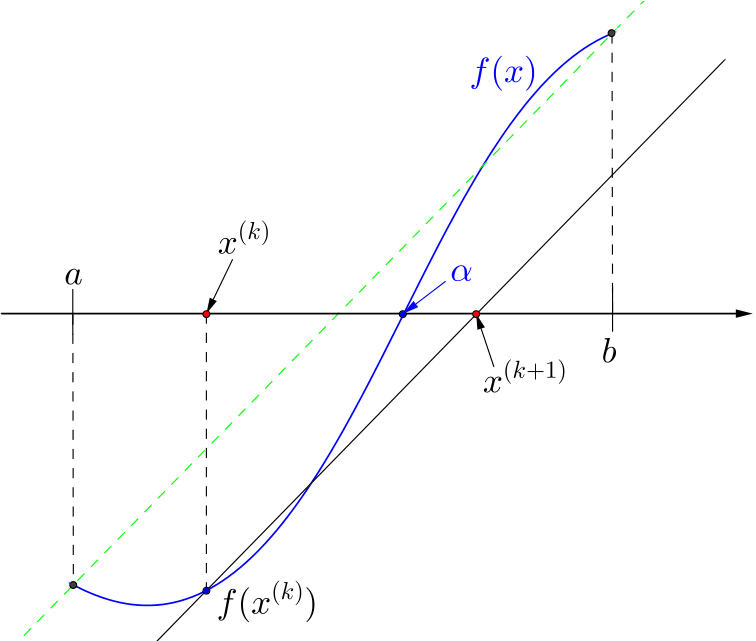
\includegraphics[width=0.68\textwidth]{chord_geometry.png}
\caption{Interpretazione geometrica del metodo delle corde: si usa la corda che unisce i punti $(a,f(a))$ e $(b,f(b))$, di pendenza costante $q$, per aggiornare l'iterata $x^{(k)}$.}
\end{figure}

\subsection{Metodo delle secanti}
Si sostituisce $f'\bigl(x^{(k)}\bigr)$ con il rapporto incrementale calcolato sulle due iterate precedenti:
\begin{formulaBox}
\[
 x^{(k+1)}=x^{(k)}-(x^{(k)}-x^{(k-1)})
 \frac{f\bigl(x^{(k)}\bigr)}{f\bigl(x^{(k)}\bigr)-f\bigl(x^{(k-1)}\bigr)},
 \qquad k\ge 0.
\]
\end{formulaBox}
In questo caso bisogna assegnare sia $x^{(0)}$ sia $x^{(-1)}$.


\begin{figure}[H]
\centering
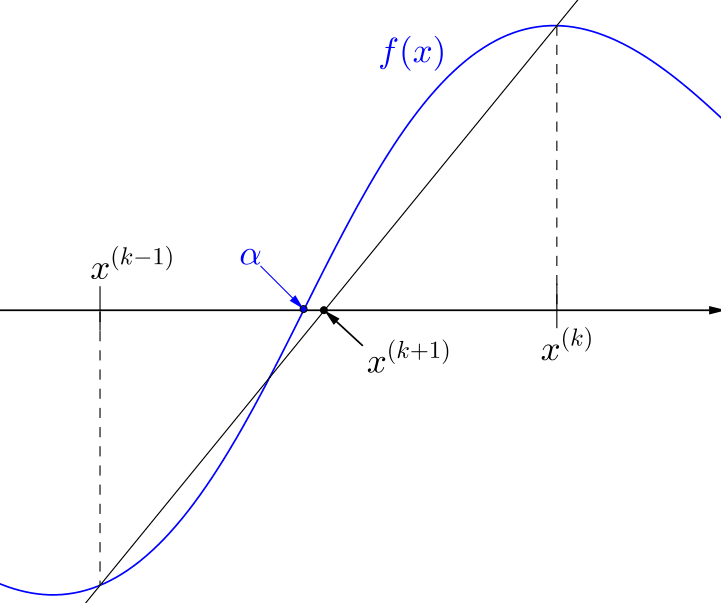
\includegraphics[width=0.60\textwidth]{secant_geometry.png}
\caption{Interpretazione geometrica del metodo delle secanti: la nuova iterata si ottiene intersecando con l'asse $x$ la secante passante per i punti corrispondenti a $x^{(k-1)}$ e $x^{(k)}$.}
\end{figure}

\section{Interpretazione come iterazioni di punto fisso}
Se $\alpha$ `e uno zero di $f$, allora il problema pu`o essere riscritto nella seguente forma:
\begin{formulaBox}
\[
\left\{
\begin{array}{l}
\text{Trovare }\alpha\text{ tale che}\\[0.2em]
 f(\alpha)=0
\end{array}
\right.
\Longleftrightarrow
\left\{
\begin{array}{l}
\text{Cercare }\alpha\text{ tale che}\\[0.2em]
 \alpha=\varphi(\alpha)\\[0.2em]
 \text{con }\varphi(x)=x-f(x)
\end{array}
\right.
\]
\end{formulaBox}

Un metodo per la ricerca dei punti fissi di una funzione $\varphi:[a,b]\to\R$ si pu`o trovare considerando il seguente metodo iterativo:
\begin{formulaBox}
\[
\left\{
\begin{array}{l}
\text{Dato }x^{(0)},\\[0.2em]
 x^{(k+1)}=\varphi(x^{(k)}),\quad k\ge 0
\end{array}
\right.
\qquad
\varphi\ \text{funzione di iterazione di punto fisso}
\]
\end{formulaBox}

Supponiamo di voler trovare lo zero di $f(x)=x-\cos(x)$. Allora se $\alpha$ `e uno zero di $f$, cio`e $f(\alpha)=\alpha-\cos(\alpha)$, si ha che $\alpha$ soddisfa
\[
 \alpha=\cos(\alpha).
\]
Detta $\varphi(x)$ la funzione di cui si cercano i punti fissi, si riconosce quindi che $\alpha$ `e punto fisso per la funzione coseno. Partendo da $x^{(0)}=1$ si genera la successione
\[
 x^{(1)}=\cos(x^{(0)})=\cos(1)=0.54030230586814,
\]
\[
 x^{(2)}=\cos(x^{(1)})=0.85755321584639,
\]
\[
 \dots,
\qquad
 x^{(20)}=\cos(x^{(19)})=0.73918439977149,
\]
che tende al valore $\alpha=0.73908513$.

\begin{figure}[H]
\centering
\begin{subfigure}{0.47\textwidth}
  \centering
  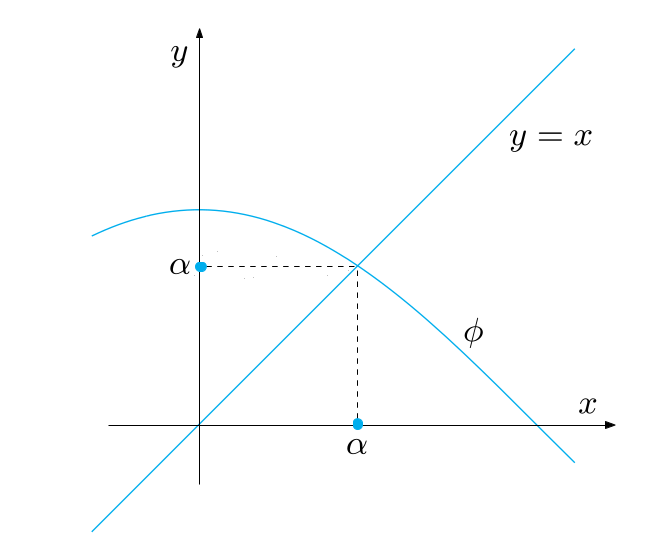
\includegraphics[width=\linewidth]{fixed_point_intro.png}
  \caption{Interpretazione geometrica di un punto fisso: l'intersezione tra $y=\varphi(x)$ e $y=x$.}
\end{subfigure}\hfill
\begin{subfigure}{0.47\textwidth}
  \centering
  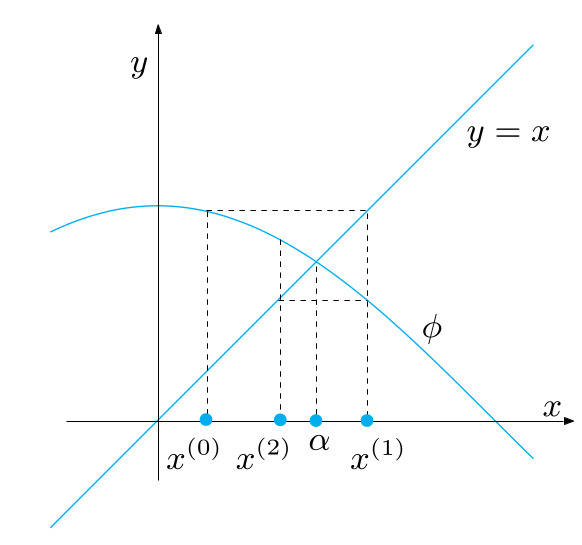
\includegraphics[width=\linewidth]{fixed_point_cobweb.png}
  \caption{Schema delle iterate di punto fisso verso $\alpha$.}
\end{subfigure}
\caption{Metodo delle iterazioni di punto fisso.}
\end{figure}

\subsection{Corde e Newton come metodi di punto fisso}
I metodi che abbiamo visto finora possono essere visti come iterazioni di punto fisso:
\begin{formulaBox}
\[
\begin{array}{ll}
1.\ \text{Metodo delle corde.} & x^{(k+1)}=x^{(k)}-\dfrac{1}{q}f(x^{(k)}),\qquad q=\dfrac{f(b)-f(a)}{b-a},\qquad \varphi_C(x)=x-\dfrac{1}{q}f(x),\\[1.0em]
2.\ \text{Metodo di Newton.} & x^{(k+1)}=x^{(k)}-\dfrac{f(x^{(k)})}{f'(x^{(k)})},\qquad \varphi_N(x)=x-\dfrac{f(x)}{f'(x)}.
\end{array}
\]
\end{formulaBox}
3. Metodo delle secanti. NON `e un metodo di punto fisso ($x^{(k+1)}$ dipende da $x^{(k)}$ ma anche da $x^{(k-1)}$).

\subsection{Esempio di assenza di convergenza per le iterazioni di punto fisso}
Non tutte le scelte di $\varphi$ producono un metodo convergente. Per esempio, se si considera
\[
 \varphi(x)=e^x,
\]
non esistono punti fissi reali, perch\'e il grafico di $y=e^x$ non interseca la retta $y=x$. Di conseguenza, l'iterazione
\[
 x^{(k+1)}=\varphi\bigl(x^{(k)}\bigr)
\]
non pu\`o convergere a un punto fisso.

\begin{figure}[H]
\centering
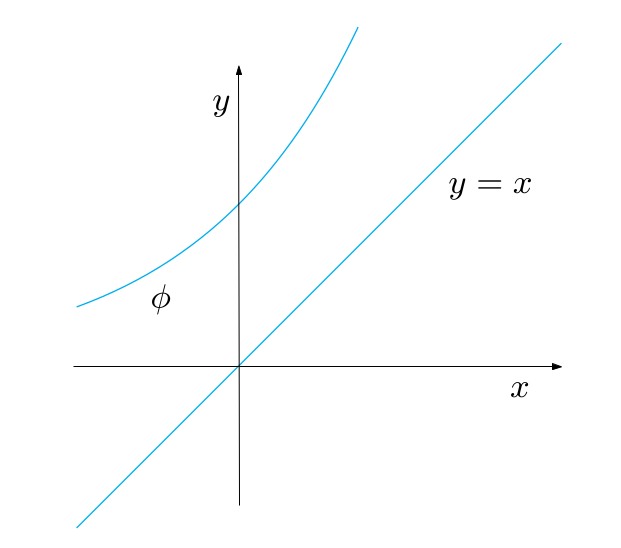
\includegraphics[width=0.45\textwidth]{fixed_point_no_convergence.png}
\caption{Caso in cui $y=\varphi(x)$ non interseca la retta $y=x$: non esistono punti fissi e le iterazioni di punto fisso non convergono.}
\end{figure}

\section{Esistenza, unicit\`a e convergenza globale su $[a,b]$}
\begin{theorem}[Esistenza e unicit\`a del punto fisso]
Sia $\varphi:[a,b]\to\R$ continua e sia $x^{(0)}\in[a,b]$ assegnato. Consideriamo le iterazioni di punto fisso
\[
 x^{(k+1)}=\varphi(x^{(k)}),\qquad k\ge 0.
\]
Allora:
\begin{enumerate}[label=\arabic*)]
  \item se $\forall x\in[a,b]$ si ha $\varphi(x)\in[a,b]$, allora $\exists$ almeno un punto fisso $\alpha\in[a,b]$;
  \item se inoltre
  \[
   \exists L<1\ \text{tale che}\ |\varphi(x_1)-\varphi(x_2)|\le L|x_1-x_2|,\qquad \forall x_1,x_2\in[a,b],
  \]
  allora
  \begin{enumerate}[label=\roman*)]
    \item $\exists!\alpha\in[a,b]$ tale che $\varphi(\alpha)=\alpha$;
    \item $\forall x^{(0)}\in[a,b]$ vale
    \[
     \lim_{k\to\infty}x^{(k)}=\alpha.
    \]
  \end{enumerate}
\end{enumerate}
\end{theorem}

\section{Convergenza locale e ordine del metodo}
Sia $\varphi:[a,b]\to\R$ funzione di iterazione e supponiamo che sia $\alpha$ un suo punto fisso. Sia inoltre $\varphi\in C^1(I_\alpha)$, dove $I_\alpha$ `e un opportuno intorno di $\alpha$.

\begin{theorem}[Convergenza locale]
\begin{enumerate}[label=\arabic*)]
  \item Se $|\varphi'(\alpha)|<1$, allora $\exists\delta>0$ tale che $\forall x^{(0)}:|x^{(0)}-\alpha|<\delta$, la successione $x^{(k)}\to\alpha$. Inoltre vale
  \[
   \lim_{k\to\infty}\frac{x^{(k+1)}-\alpha}{(x^{(k)}-\alpha)^1}=\varphi'(\alpha),
  \]
  ordine $1$.
  \item Se inoltre $\varphi\in C^2(I_\alpha)$ e $\varphi'(\alpha)=0$, $\varphi''(\alpha)\neq 0$, allora vale
  \[
   \lim_{k\to\infty}\frac{x^{(k+1)}-\alpha}{(x^{(k)}-\alpha)^2}=\frac{\varphi''(\alpha)}{2},
  \]
  ordine $2$.
\end{enumerate}
\end{theorem}

Le precedenti relazioni valgono per $k\to\infty$. Per un generico $k$ possiamo scrivere le seguenti disuguaglianze:
\begin{enumerate}[label=\arabic*)]
  \item se $|\varphi'(\alpha)|<1$, allora
  \[
   |x^{(k+1)}-\alpha|\le |\varphi'(\alpha)|\,|x^{(k)}-\alpha|,
  \]
  cio`e l'errore al passo $k+1$ scala linearmente rispetto all'errore al passo $k$ (ordine $1$);
  \item se inoltre $\varphi\in C^2(I_\alpha)$ e $\varphi'(\alpha)=0$, $\varphi''(\alpha)\neq 0$, allora
  \[
   |x^{(k+1)}-\alpha|\le \frac{|\varphi''(\alpha)|}{2}|x^{(k)}-\alpha|^2,
  \]
  cio`e l'errore al passo $k+1$ scala quadraticamente rispetto all'errore al passo $k$ (ordine $2$).
\end{enumerate}

\subsection{Esempio di mancata convergenza}
Consideriamo
\[
 \varphi(x)=x^2-1.
\]
I punti fissi soddisfano
\[
 \alpha=\alpha^2-1,
\]
perci\`o
\[
 \alpha_{1,2}=\frac{1\pm\sqrt5}{2}.
\]
Tuttavia, scegliendo $x^{(0)}=1$, le iterate diventano
\[
 x^{(1)}=0,
 \qquad x^{(2)}=-1,
 \qquad x^{(3)}=0,
\]
e il processo non converge. La ragione \`e che
\[
 \varphi'(x)=2x,
 \qquad
 \varphi'(\alpha_{1,2})=1\pm\sqrt5,
\]
quindi
\[
 |\varphi'(\alpha_{1,2})|>1.
\]

\section{Applicazione del teorema ai metodi classici}

\subsection{Metodo delle corde}
Per il metodo delle corde si ha
\[
 \varphi_C(x)=x-\frac1q f(x),
 \qquad
 \varphi_C'(x)=1-\frac1q f'(x),
 \qquad
 q=\frac{f(b)-f(a)}{b-a}.
\]
Se $\alpha$ \`e uno zero di $f$ e $f'(\alpha)\neq 0$, la convergenza richiede
\[
 \left|1-\frac1q f'(\alpha)\right|<1.
\]
Questa condizione equivale a chiedere che:
\begin{enumerate}[label=(\roman*)]
  \item $q$ e $f'(\alpha)$ abbiano lo stesso segno;
  \item valga la stima
  \[
  \frac{b-a}{f(b)-f(a)}f'(\alpha)<2.
  \]
\end{enumerate}
Se tali ipotesi sono soddisfatte, il metodo delle corde ha convergenza lineare.

\subsection{Metodo di Newton}
Per Newton
\[
 \varphi_N(x)=x-\frac{f(x)}{f'(x)}.
\]
Derivando si ottiene
\[
 \varphi_N'(x)=\frac{f(x)f''(x)}{[f'(x)]^2}.
\]
Se $\alpha$ \`e una radice semplice, cio\`e
\[
 f(\alpha)=0,
 \qquad
 f'(\alpha)\neq 0,
\]
allora
\[
 \varphi_N'(\alpha)=0,
\]
mentre
\[
 \varphi_N''(\alpha)=\frac{f''(\alpha)}{f'(\alpha)}\neq 0.
\]
Per il teorema di convergenza locale, il metodo di Newton converge localmente ed \`e di ordine $2$.

\subsection{Metodo di Newton modificato}
Se $\alpha$ ha molteplicit\`a $m>1$ (cio`e se le derivate $f^{(j-1)}(\alpha)=0$, $j\le m$), allora Newton converge ancora, ma non `e pi`u del secondo ordine. Infatti, in generale, si pu`o dimostrare che
\[
 \varphi_N'(\alpha)=1-\frac{1}{m}.
\]
Quindi, per ripristinare l'ordine di convergenza, si modifica il metodo di Newton nel seguente modo
\begin{formulaBox}
\[
 x^{(k+1)}=x^{(k)}-m\frac{f(x^{(k)})}{f'(x^{(k)})},
 \qquad
 \varphi_{N\mathrm{mod}}(x)=x-m\frac{f(x)}{f'(x)}.
\]
\end{formulaBox}
Il valore di $m$ `e spesso a priori incognito; ci vogliono stime numeriche.

% Nei lucidi le pagine 29--31 riportano una dimostrazione testuale del fatto che
% \varphi'_N(\alpha)=1-1/m, ma non sono racchiuse in un box rosso; per la richiesta
% dell'utente non vengono evidenziate come contenuto non d'esame.

\section{Criteri d'arresto}
Sia $e^{(k)}=\alpha-x^{(k)}$ l'errore al passo $k$.
Poich\'e un metodo iterativo pu\`o essere eseguito solo per un numero finito di passi, bisogna introdurre criteri pratici di arresto.

\subsection{Criterio sul residuo}
Si fissa una tolleranza $\varepsilon>0$ e si arresta il metodo quando
\begin{formulaBox}
\[
 |f\bigl(x^{(k)}\bigr)|<\varepsilon.
\]
\end{formulaBox}
Il criterio ha interpretazione diversa a seconda del valore di $|f'(\alpha)|$:
\begin{itemize}
  \item se $|f'(\alpha)|\approx 1$, allora $|e^{(k)}|\approx \varepsilon$ e il test \`e soddisfacente;
  \item se $|f'(\alpha)|\ll 1$, il test pu\`o essere inaffidabile perch\'e potrebbe valere $|e^{(k)}|\gg \varepsilon$;
  \item se $|f'(\alpha)|\gg 1$, il test \`e restrittivo: si ha $|e^{(k)}|\ll \varepsilon$, ma il criterio resta valido.
\end{itemize}


\begin{figure}[H]
\centering
\begin{subfigure}{0.46\textwidth}
  \centering
  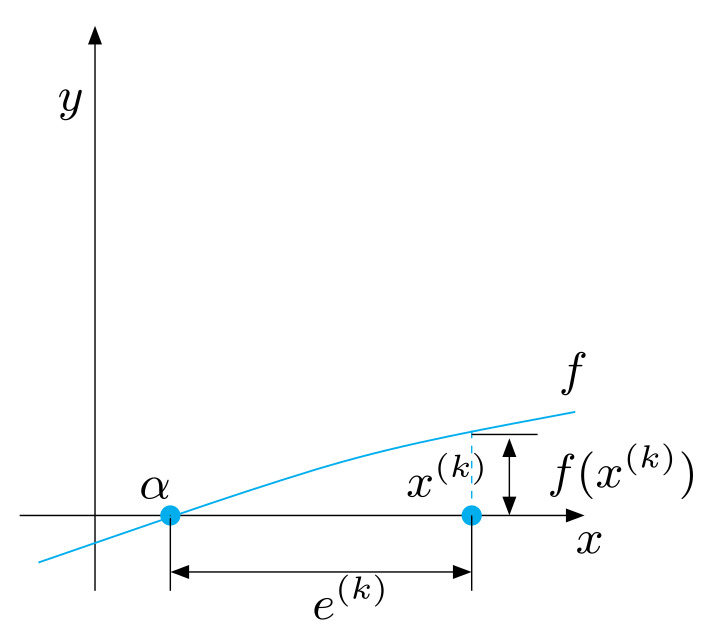
\includegraphics[width=\linewidth]{residual_criterion_flat_slope.png}
  \caption{Se $|f'(\alpha)|\ll 1$, un residuo piccolo non garantisce un errore piccolo.}
\end{subfigure}\hfill
\begin{subfigure}{0.46\textwidth}
  \centering
  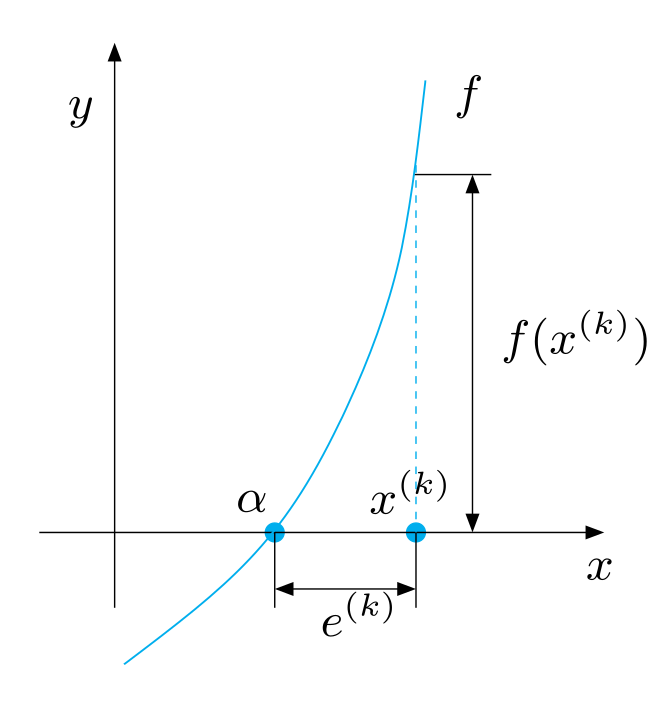
\includegraphics[width=\linewidth]{residual_criterion_steep_slope.png}
  \caption{Se $|f'(\alpha)|\gg 1$, il criterio sul residuo \'e prudente ma affidabile.}
\end{subfigure}
\caption{Criterio sul residuo.}
\end{figure}

\subsection{Criterio sull'incremento}
Si fissa una tolleranza $\varepsilon>0$ e si arresta il metodo quando
\begin{formulaBox}
\[
 |x^{(k+1)}-x^{(k)}|<\varepsilon.
\]
\end{formulaBox}
Le conclusioni principali dei lucidi sono:
\begin{itemize}
  \item se $-1<\varphi'(\alpha)<0$, il test \`e soddisfacente;
  \item per i metodi del secondo ordine vale $\varphi'(\alpha)=0$, quindi il test funziona bene (in particolare per Newton);
  \item se $\varphi'(\alpha)\approx 1$, il test \`e insoddisfacente.
\end{itemize}
Se $\varphi'$ varia poco in un intorno di $\alpha$, si ottiene anche la stima approssimata
\[
 \alpha-x^{(k)}\approx \frac{1}{1-\varphi'(\alpha)}\bigl(x^{(k+1)}-x^{(k)}\bigr),
\]
che spiega perch\'e l'incremento sia un buon indicatore dell'errore quando $\varphi'(\alpha)$ \`e vicino a $0$.


\chapter{Metodi numerici per sistemi non lineari}

\section{Dal caso scalare ai sistemi}
Consideriamo il sistema non lineare in due incognite
\[
\begin{cases}
 x_1^2-2x_1x_2=2,\
 x_1+x_2^2=-1.
\end{cases}
\]
Ponendo
\[
 f_1(x_1,x_2)=x_1^2-2x_1x_2-2,
 \qquad
 f_2(x_1,x_2)=x_1+x_2^2+1,
\]
il precedente sistema pu`o essere riscritto equivalentemente come
\[
\begin{cases}
 f_1(x_1,x_2)=0,\
 f_2(x_1,x_2)=0,
\end{cases}
\]
e, ponendo $f=(f_1,f_2)$ e $x=(x_1,x_2)$, anche come
\begin{formulaBox}
\[
 f(x)=0.
\]
\end{formulaBox}
Geometricamente, le equazioni $f_1(x_1,x_2)=0$ e $f_2(x_1,x_2)=0$ rappresentano due curve nel piano; le loro intersezioni sono le radici del sistema.

\begin{figure}[H]
\centering
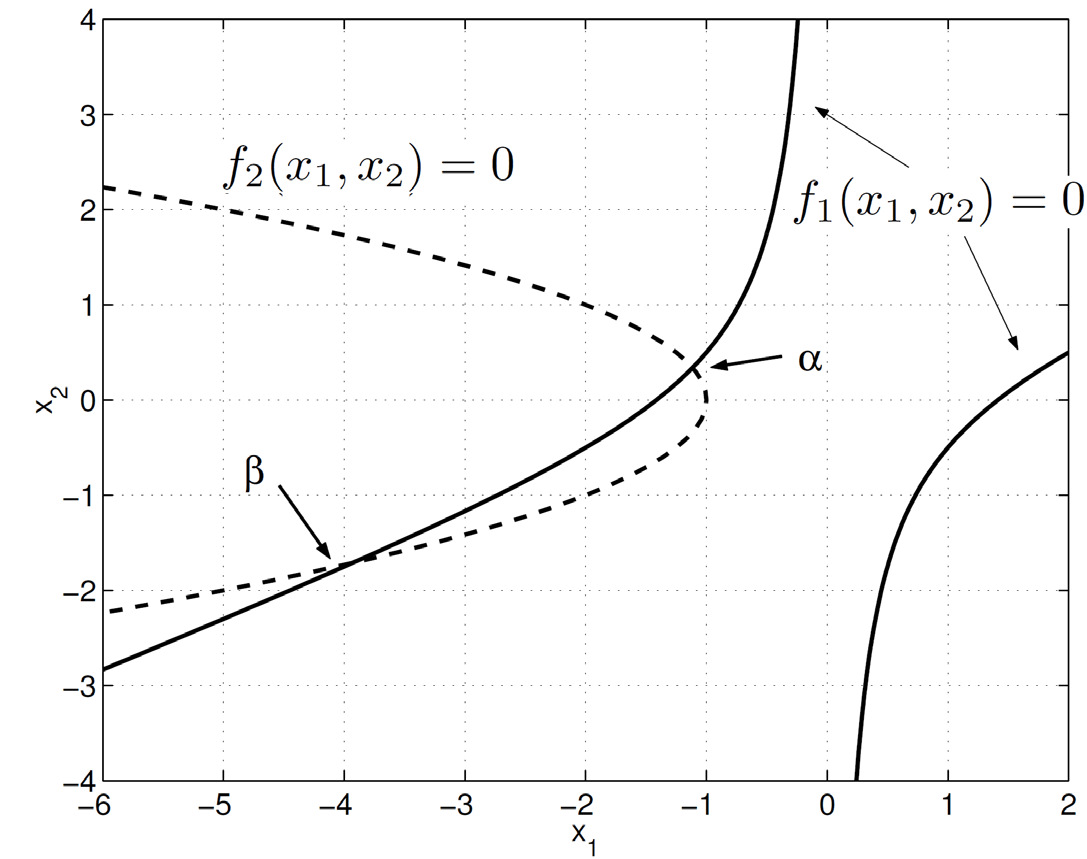
\includegraphics[width=0.78\textwidth]{nonlinear_system_curves.png}
\caption{Interpretazione geometrica di un sistema non lineare in due variabili: le intersezioni tra le curve $f_1(x_1,x_2)=0$ e $f_2(x_1,x_2)=0$ corrispondono alle radici del sistema.}
\end{figure}

\section{Formulazione generale}
In generale abbiamo il seguente problema
\[
 f(x)=0
 \qquad \Longleftrightarrow \qquad
 \left\{
 \begin{array}{l}
  f_1(x_1,\dots,x_j,\dots,x_n)=0,\\
  \vdots\\
  f_i(x_1,\dots,x_j,\dots,x_n)=0,\\
  \vdots\\
  f_n(x_1,\dots,x_j,\dots,x_n)=0,
 \end{array}
 \right.
\]
dove $x\in\R^n$ `e il vettore delle incognite $x_j$, $f:\R^n\to\R^n$ e le $f_i$ esprimono relazioni non lineari fra le incognite.
Le difficolt\`a dal punto di vista numerico sono due:
\begin{enumerate}[label=\alph*)]
  \item `e un sistema, quindi abbiamo equazioni accoppiate;
  \item `e non lineare, quindi va linearizzato.
\end{enumerate}

\section{Metodo di Newton per sistemi non lineari}
Nel caso scalare, il metodo di Newton pu\`o essere scritto come
\[
 f'\bigl(x^{(k)}\bigr)\,\delta x^{(k)}=-f\bigl(x^{(k)}\bigr),
 \qquad
 x^{(k+1)}=x^{(k)}+\delta x^{(k)}.
\]
L'analogo per i sistemi si ottiene introducendo la matrice Jacobiana.

\subsection{Matrice Jacobiana}
Dato un punto $z\in\R^n$, introduciamo la matrice Jacobiana relativa a $f$:
\[
 J(z)=\nabla f(z)
\]
di componenti
\[
 J_{i\ell}=\frac{\partial f_i(z)}{\partial x_\ell},\qquad i,\ell=1,\dots,n.
\]
Per ogni $z\in\R^n$ si ha quindi $J(z)\in\R^{n\times n}$.

\subsection{Algoritmo di Newton}
Dato $x^{(0)}$, se $J(x^{(k)})$ `e una matrice non singolare, per ogni $k$ risolvo:
\begin{formulaBox}
\[
 J(x^{(k)})\,\delta x^{(k)}=-f(x^{(k)}),
 \qquad
 x^{(k+1)}=x^{(k)}+\delta x^{(k)}.
\]
\end{formulaBox}
Ad ogni iterazione $k$, il primo passo del metodo di Newton consiste quindi nella risoluzione di un sistema lineare di dimensione $n$. Una volta risolto il sistema lineare e ottenuto $\delta x^{(k)}$, aggiorno la $x^{(k+1)}$ mediante il secondo passo del metodo.

\section{Convergenza del metodo di Newton per sistemi}
Analogamente al caso scalare, il metodo di Newton per sistemi `e:
\begin{itemize}
  \item un \emph{metodo locale}: $\exists\delta>0$ tale che, se
  \[
   \|\alpha-x^{(0)}\|<\delta,
  \]
  allora si ha convergenza
  \[
   \lim_{k\to\infty}\|\alpha-x^{(k)}\|=0;
  \]
  \item un \emph{metodo del secondo ordine}: se converge e $J$ `e derivabile, allora si ha
  \[
   \frac{\|\alpha-x^{(k+1)}\|}{\|\alpha-x^{(k)}\|^2}\le C.
  \]
\end{itemize}

\section{Esempio esplicito}
Riprendiamo il sistema in due incognite introdotto all'inizio del capitolo.
La Jacobiana \`e
\[
 J(x)=
 \begin{bmatrix}
  2x_1-2x_2 & -2x_1\\
  1 & 2x_2
 \end{bmatrix}.
\]
Se scegliamo come punto iniziale
\[
 x^{(0)}=
 \begin{bmatrix}
 1\\ 1
 \end{bmatrix},
\]
allora
\[
 f\bigl(x^{(0)}\bigr)=
 \begin{bmatrix}
 -3\\ 3
 \end{bmatrix},
 \qquad
 J\bigl(x^{(0)}\bigr)=
 \begin{bmatrix}
 0 & -2\\
 1 & 2
 \end{bmatrix}.
\]
La prima iterazione \`e data da
\[
 J\bigl(x^{(0)}\bigr)\,\delta x^{(0)}=-f\bigl(x^{(0)}\bigr),
\]
ossia
\[
 \begin{bmatrix}
 0 & -2\\
 1 & 2
 \end{bmatrix}
 \begin{bmatrix}
 \delta x_1^{(0)}\\ \delta x_2^{(0)}
 \end{bmatrix}
 =
 \begin{bmatrix}
 3\\ -3
 \end{bmatrix}.
\]
La soluzione del sistema lineare \`e
\[
 \delta x_1^{(0)}=0,
 \qquad
 \delta x_2^{(0)}=-\frac32,
\]
quindi
\[
 x^{(1)}=x^{(0)}+\delta x^{(0)}=
 \begin{bmatrix}
 1\\ -\frac12
 \end{bmatrix}.
\]
Alla successiva iterazione si ha
\[
 f\bigl(x^{(1)}\bigr)=
 \begin{bmatrix}
 0\\ \frac94
 \end{bmatrix},
 \qquad
 J\bigl(x^{(1)}\bigr)=
 \begin{bmatrix}
 3 & -2\\
 1 & -1
 \end{bmatrix},
\]
e il procedimento prosegue in modo analogo.

\section{Criteri di arresto}
Anche per i sistemi non lineari, essendo il metodo di Newton iterativo, si utilizzano criteri di arresto analoghi al caso scalare.
Per una tolleranza assegnata $\varepsilon>0$ si impiegano tipicamente:
\begin{itemize}
  \item il \emph{criterio sul residuo}
  \[
  \|f\bigl(x^{(k)}\bigr)\|<\varepsilon;
  \]
  \item il \emph{criterio sull'incremento}
  \[
  \|x^{(k+1)}-x^{(k)}\|<\varepsilon.
  \]
\end{itemize}

\section{Costo computazionale}
A ogni iterazione il metodo di Newton richiede la costruzione della Jacobiana e la risoluzione del sistema lineare associato. Per questo i lucidi sintetizzano il costo come
\begin{formulaBox}
\[
 \text{CPU TIME}=\#\mathrm{iter}\times (C_{\mathrm{cos}}+C_{\mathrm{sl}}),
\]
\end{formulaBox}
dove $C_{\mathrm{cos}}$ \`e il tempo necessario per costruire $J\bigl(x^{(k)}\bigr)$ e $C_{\mathrm{sl}}$ \`e il costo di risoluzione del corrispondente sistema lineare.
Il numero di iterazioni \`e in genere basso, perch\'e Newton \`e di ordine $2$, ma il tempo complessivo pu\`o restare elevato se la Jacobiana \`e costosa da costruire o se i sistemi lineari sono grandi.

\section{Varianti del metodo di Newton}

\subsection{Aggiornamento della Jacobiana ogni $p$ iterazioni}
Una prima variante consiste nell'aggiornare la Jacobiana solo ogni $p$ passi.
In questo modo il costo medio di costruzione si riduce di un fattore circa $p$.
Se inoltre i sistemi lineari vengono risolti mediante fattorizzazione LU, il costo della fattorizzazione
\[
 \frac23 n^3
\]
viene di fatto distribuito su $p$ iterazioni, producendo un costo medio addizionale pari a
\[
 \frac{2n^3}{3p}
\]
per iterazione.
Il prezzo da pagare \`e un aumento del numero di iterazioni: il metodo non \`e pi\`u del secondo ordine e, se $p$ \`e troppo grande, si pu\`o addirittura perdere la convergenza.

\subsection{Inexact Newton}
Una seconda idea consiste nel sostituire, a ogni passo, la Jacobiana con una sua approssimazione $B_k$, facile da costruire e tale che il sistema lineare associato sia facilmente risolvibile.
Il numero di iterazioni cresce rispetto a Newton classico e l'ordine di convergenza scende sotto $2$, ma la speranza \`e che il costo complessivo diminuisca.

\begin{noteBox}
Nonostante il nome, \emph{inexact Newton} resta un metodo esatto nel senso che, se converge, la soluzione limite \`e ancora una radice del sistema non lineare. L'aggettivo \emph{inexact} si riferisce solo all'uso di una Jacobiana approssimata.
\end{noteBox}

\subsection{Metodo di Broyden}
Uno dei pi\`u noti metodi inexact-Newton \`e quello di Broyden, che generalizza il metodo delle secanti.
Dato $B_k$, si eseguono i passi
\begin{formulaBox}
\[
 B_k\,\delta x^{(k)}=-f\bigl(x^{(k)}\bigr),
\]
\[
 x^{(k+1)}=x^{(k)}+\delta x^{(k)},
 \qquad
 \delta f^{(k)}=f\bigl(x^{(k+1)}\bigr)-f\bigl(x^{(k)}\bigr),
\]
\[
 B_{k+1}=B_k+
 \frac{\bigl(\delta f^{(k)}-B_k\delta x^{(k)}\bigr)(\delta x^{(k)})\trans}
 {(\delta x^{(k)})\trans\delta x^{(k)}}.
\]
\end{formulaBox}
Il metodo di Broyden \`e superlineare (ordine maggiore di $1$), ma non del secondo ordine.




\chapter{Approssimazione di dati e funzioni}

\section{Esempi introduttivi}
Il problema dell'approssimazione nasce quando si conoscono solo un numero finito di informazioni su una quantit\`a di interesse e si vuole comunque ottenere una descrizione utile, stabile e con carattere predittivo.
Nei lucidi il tema viene introdotto con esempi in cui i dati disponibili sono o misure sperimentali oppure valori di una funzione noti solo in alcuni nodi.

\subsection{Esempio: sforzo e deformazione di un disco intervertebrale}
Supponiamo di aver effettuato un esperimento per studiare il legame tra lo sforzo $\sigma$ e la deformazione $\varepsilon$ di un disco intervertebrale. In questo contesto si introducono le grandezze
\[
 \sigma=\frac{F}{A},
 \qquad
 \varepsilon=\frac{\Delta L}{L}.
\]
Dai lucidi si ricavano otto misure sperimentali, che qui riportiamo in tabella:

\begin{figure}[H]
\centering
\begin{subfigure}{0.42\textwidth}
  \centering
  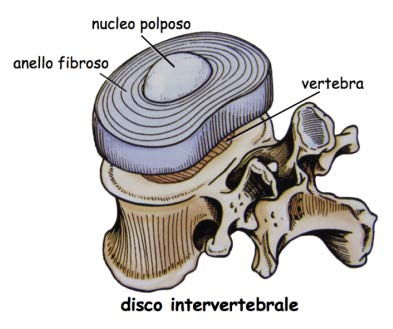
\includegraphics[width=0.95\linewidth]{ch3_disk_intervertebral.png}
  \caption{Schema del disco intervertebrale.}
\end{subfigure}\hfill
\begin{subfigure}{0.50\textwidth}
  \centering
  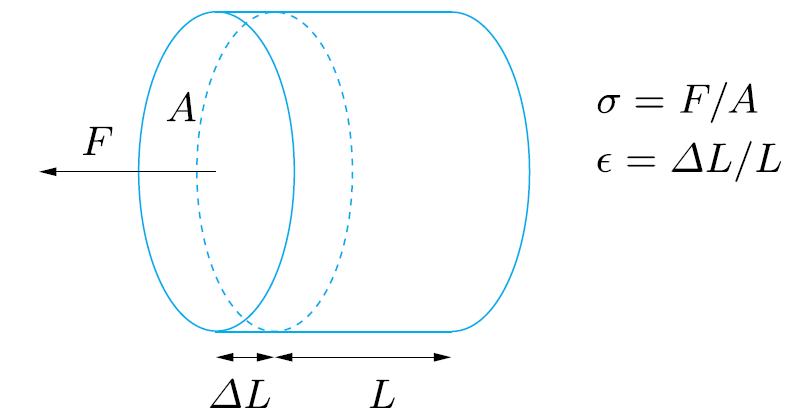
\includegraphics[width=\linewidth]{ch3_stress_strain_scheme.png}
  \caption{Definizione di sforzo e deformazione.}
\end{subfigure}
\caption{Primo esempio motivazionale del capitolo: misure sperimentali sforzo-deformazione.}
\end{figure}

\begin{center}
\begin{tabular}{ccccccccc}
\toprule
$i$ & 0 & 1 & 2 & 3 & 4 & 5 & 6 & 7\\
\midrule
$x_i=\sigma_i$ & 0.00 & 0.06 & 0.14 & 0.25 & 0.31 & 0.47 & 0.60 & 0.70\\
$y_i=\varepsilon_i$ & 0.00 & 0.08 & 0.14 & 0.20 & 0.23 & 0.25 & 0.28 & 0.29\\
\bottomrule
\end{tabular}
\end{center}

Poich\'e il legame sforzo--deformazione \`e approssimativamente lineare per deformazioni non troppo grandi, ha senso cercare una retta che approssimi bene le misure e usarla per stimare la deformazione corrispondente a uno stato di sforzo non misurato direttamente. In questo caso l'approssimante non passa necessariamente per tutti i dati: si entra nel contesto dei \emph{minimi quadrati}.

\begin{figure}[H]
\centering
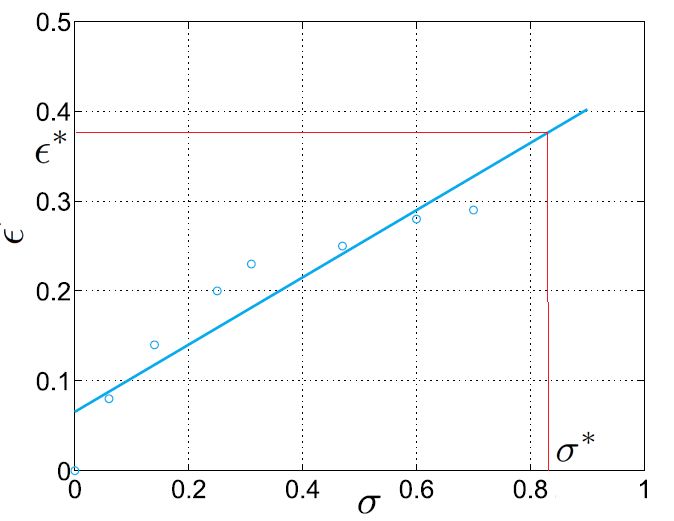
\includegraphics[width=0.58\textwidth]{ch3_regression_plot.png}
\caption{Retta approssimante per i dati sperimentali: la deformazione $\varepsilon^\ast$ si stima valutando l'approssimante in corrispondenza di uno sforzo assegnato $\sigma^\ast$.}
\end{figure}

\subsection{Esempio: approssimare una funzione nota solo in alcuni punti}
Un secondo scenario consiste nel conoscere una funzione solo in un numero finito di nodi e nel voler costruire una nuova funzione che approssimi bene i valori noti e permetta di stimare il comportamento altrove. Nei lucidi questo \`e l'esempio che porta naturalmente all'interpolazione Lagrangiana.

\begin{figure}[H]
\centering
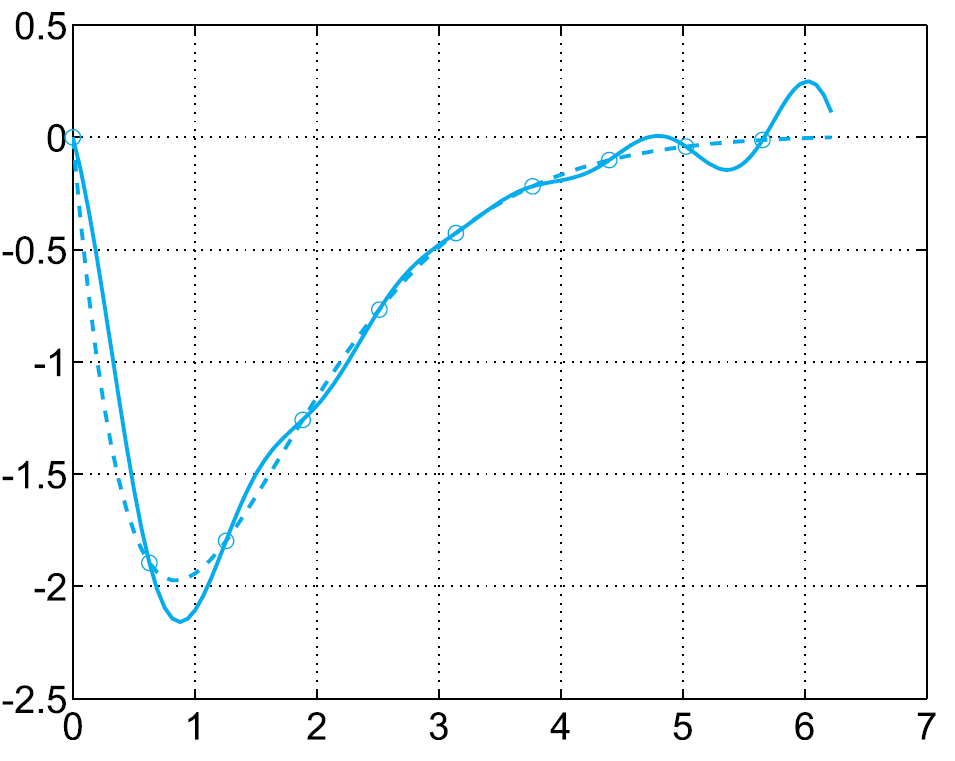
\includegraphics[width=0.58\textwidth]{ch3_function_example.png}
\caption{Funzione nota in alcuni nodi e funzione approssimante interpolante.}
\end{figure}

\section{Posizione del problema}
Supponiamo di conoscere $n+1$ coppie di dati
\[
 (x_i,y_i), \qquad i=0,\dots,n.
\]
Queste coppie possono rappresentare due casi distinti:
\begin{enumerate}[label=\arabic*)]
  \item \textbf{Misure sperimentali} di una certa quantit\`a in corrispondenza dei nodi $x_i$;
  \item \textbf{Valori di una funzione}, nel caso in cui $y_i=f(x_i)$ per una funzione assegnata $f$.
\end{enumerate}
Nel primo caso si lavora su dati affetti da errore sperimentale; nel secondo caso si dispone di campionamenti esatti della funzione nei nodi.

\begin{figure}[H]
\centering
\begin{subfigure}{0.46\textwidth}
  \centering
  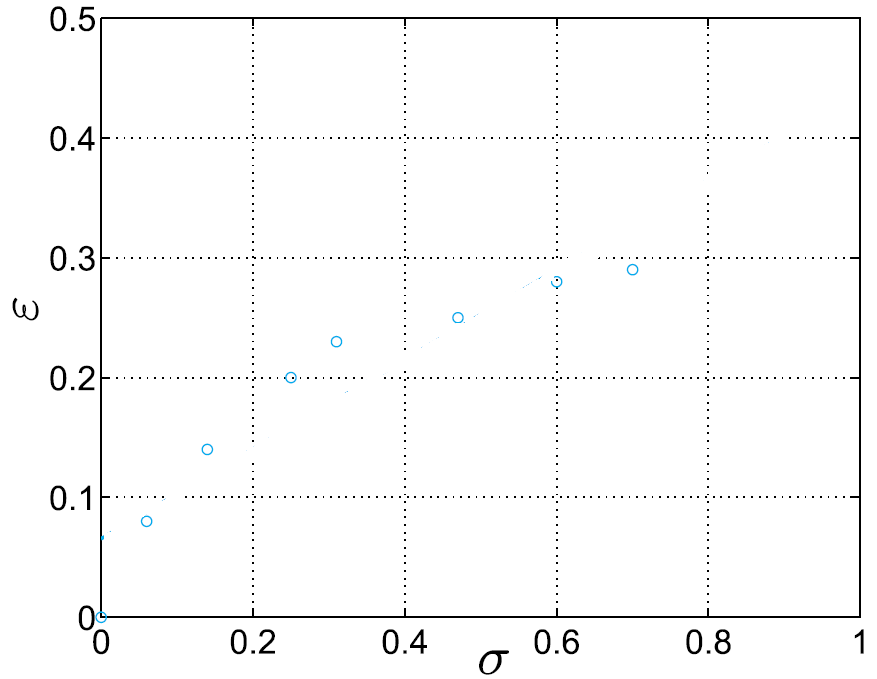
\includegraphics[width=\linewidth]{ch3_measurements_scatter.png}
  \caption{Dati sperimentali del disco intervertebrale.}
\end{subfigure}\hfill
\begin{subfigure}{0.46\textwidth}
  \centering
  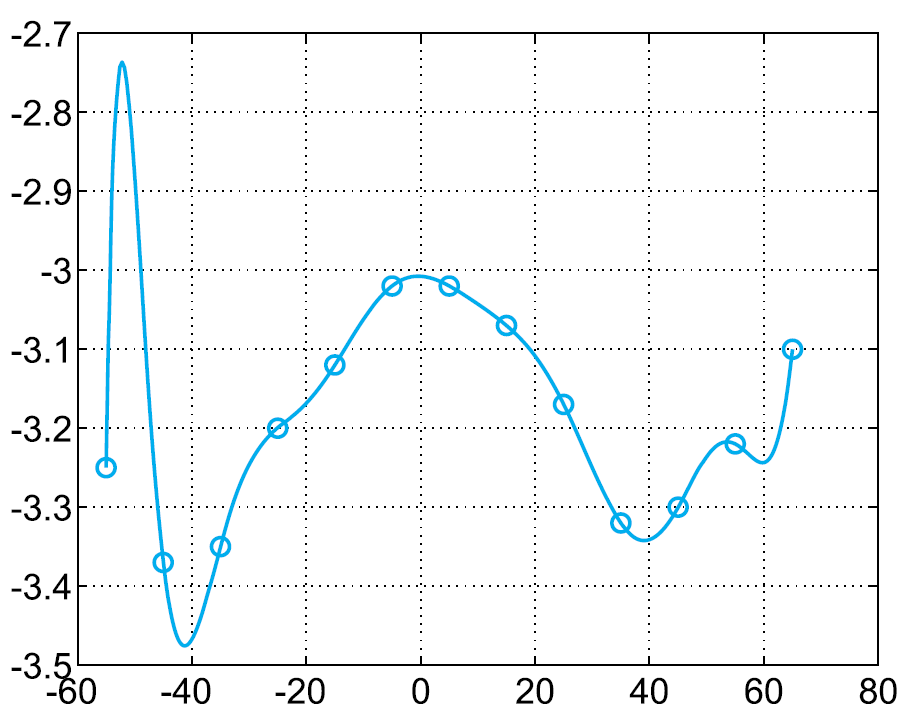
\includegraphics[width=\linewidth]{ch3_function_values_scatter.png}
  \caption{Valori campionati di una funzione in alcuni nodi.}
\end{subfigure}
\caption{Le due situazioni fondamentali considerate nel capitolo: approssimazione di dati e approssimazione di una funzione.}
\end{figure}

Il problema dell'approssimazione consiste nel determinare una funzione $\widetilde f(x)$ con buone propriet\`a di approssimazione dei dati, in modo da poter fornire stime attendibili anche fuori dai nodi disponibili.

\section{Approssimanti di tipo interpolatorio}
Date le coppie $(x_i,y_i)$, si dice che un'approssimante $\widetilde f(x)$ \`e di tipo interpolatorio se verifica
\begin{formulaBox}
\[
 \widetilde f(x_i)=y_i, \qquad i=0,\dots,n.
\]
\end{formulaBox}
Un interpolatore assume quindi esattamente il valore dei dati in corrispondenza dei nodi. Questa \`e la scelta adottata quando si vuole costruire una funzione che passi per tutte le informazioni disponibili.

\section{Polinomi caratteristici di Lagrange}
Associati ai dati $(x_i,y_i)$ si introducono i polinomi caratteristici di Lagrange
\begin{formulaBox}
\[
 \varphi_k(x)=\prod_{\substack{j=0 \\ j\ne k}}^n \frac{x-x_j}{x_k-x_j},
 \qquad k=0,\dots,n.
\]
\end{formulaBox}
Ogni $\varphi_k$ \`e un polinomio di grado $n$ e soddisfa la propriet\`a fondamentale
\[
 \varphi_k(x_i)=\delta_{ik}=
 \begin{cases}
 1 & \text{se } i=k,\\
 0 & \text{se } i\ne k.
 \end{cases}
\]
In particolare, ciascun polinomio vale $1$ nel proprio nodo e $0$ in tutti gli altri.

\begin{figure}[H]
\centering
\begin{subfigure}{0.47\textwidth}
  \centering
  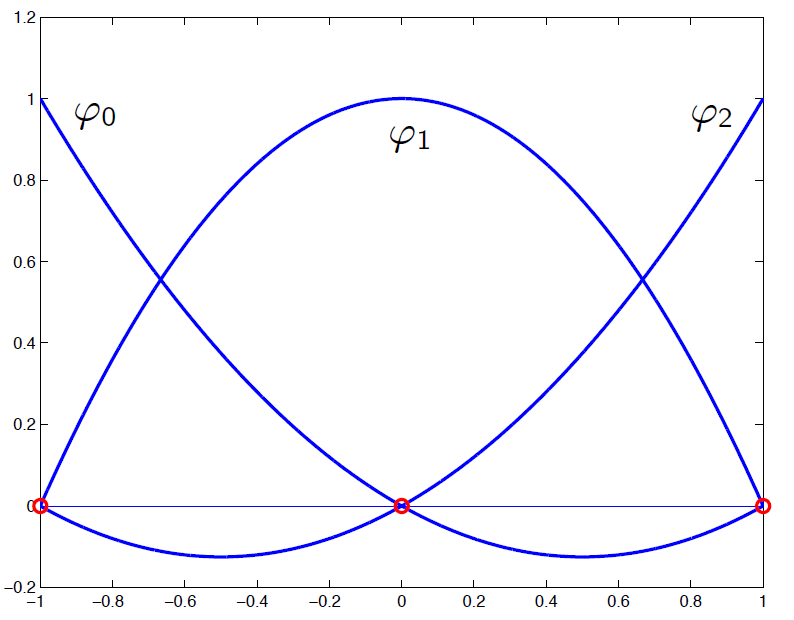
\includegraphics[width=\linewidth]{ch3_lagrange_basis_n2.png}
  \caption{Polinomi caratteristici per $n=2$.}
\end{subfigure}\hfill
\begin{subfigure}{0.47\textwidth}
  \centering
  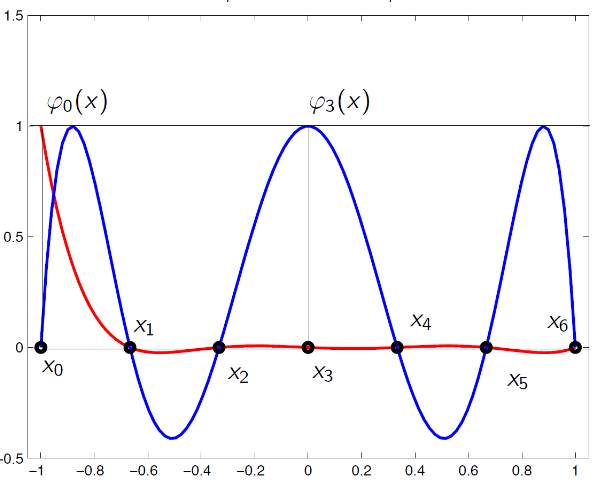
\includegraphics[width=\linewidth]{ch3_lagrange_basis_n6.png}
  \caption{Polinomi caratteristici per $n=6$.}
\end{subfigure}
\caption{Esempi di polinomi caratteristici di Lagrange.}
\end{figure}

\section{Interpolatore Lagrangiano}
L'interpolatore Lagrangiano degli $n+1$ dati \`e definito da
\begin{formulaBox}
\[
 \Pi_n(x)=\sum_{j=0}^n y_j\,\varphi_j(x).
\]
\end{formulaBox}
Se i dati provengono da una funzione $f$, cio\`e se $y_j=f(x_j)$, si usa spesso la notazione $\Pi_n f(x)$.

\begin{figure}[H]
\centering
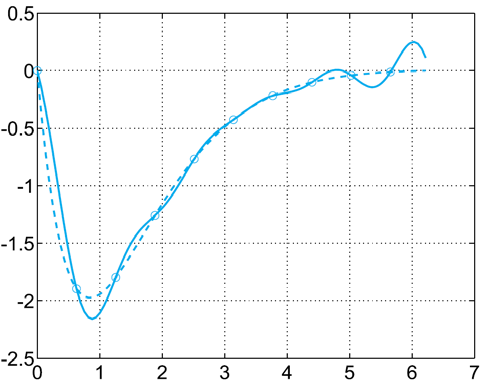
\includegraphics[width=0.62\textwidth]{ch3_lagrange_interp_intro.png}
\caption{Costruzione dell'interpolatore Lagrangiano: la funzione approssimante passa per i valori noti nei nodi.}
\end{figure}

Le propriet\`a principali dell'interpolatore Lagrangiano sono:
\begin{enumerate}[label=\arabic*)]
  \item $\Pi_n$ \`e un \textbf{interpolatore}, cio\`e $\Pi_n(x_i)=y_i$ per ogni $i$;
  \item $\Pi_n$ \`e un \textbf{polinomio di grado} al pi\`u $n$;
  \item $\Pi_n$ \`e l'\textbf{unico} polinomio di grado al pi\`u $n$ che interpola gli $n+1$ dati.
\end{enumerate}
L'unicit\`a si dimostra osservando che, se esistessero due polinomi interpolanti di grado $n$, la loro differenza sarebbe un polinomio di grado $n$ con $n+1$ zeri distinti, quindi necessariamente nullo.

\section{Accuratezza dell'interpolatore Lagrangiano}
Nel caso in cui i dati siano generati da una funzione $f$, l'errore puntuale di interpolazione si pu\`o scrivere come
\begin{formulaBox}
\[
 E_n f(x)=f(x)-\Pi_n f(x)=\frac{f^{(n+1)}(\xi_x)}{(n+1)!}\prod_{i=0}^n (x-x_i),
\]
\end{formulaBox}
dove $\xi_x$ \`e un opportuno punto dell'intervallo considerato. Questa formula mostra che l'errore dipende sia dalla regolarit\`a della funzione, sia dalla scelta dei nodi attraverso il prodotto nodale $\prod_{i=0}^n (x-x_i)$.

\begin{figure}[H]
\centering
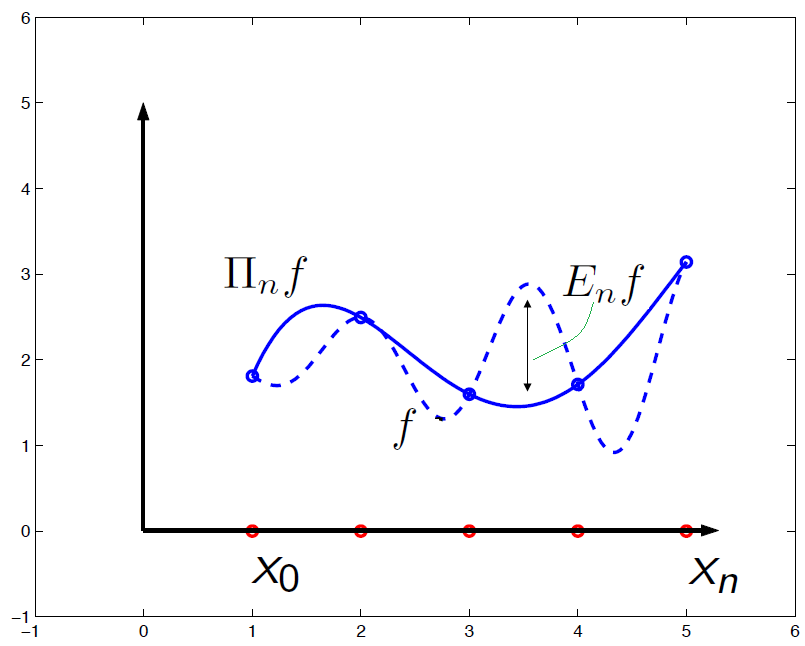
\includegraphics[width=0.55\textwidth]{ch3_pointwise_error.png}
\caption{Errore puntuale $E_n f(x)$: esso si annulla nei nodi ma in generale \`e diverso da zero tra un nodo e l'altro.}
\end{figure}

Nel caso di nodi equispaziati, se $x_{j+1}-x_j=h$ per ogni $j$, i lucidi riportano la stima
\[
 \left|\prod_{i=0}^n (x-x_i)\right|\le \frac{n!}{4}h^{n+1},
\]
che porta al seguente limite superiore per l'errore massimo:
\begin{formulaBox}
\[
 \max_{x\in I}|E_n f(x)|
 \le
 \frac{\max_{x\in I}|f^{(n+1)}(x)|}{4(n+1)}\,h^{n+1}.
\]
\end{formulaBox}
La stima suggerisce che la convergenza non \`e automatica: anche se $h\to 0$ quando $n\to\infty$, non si ha alcuna garanzia a priori che il termine contenente $f^{(n+1)}$ resti limitato.

\begin{figure}[H]
\centering
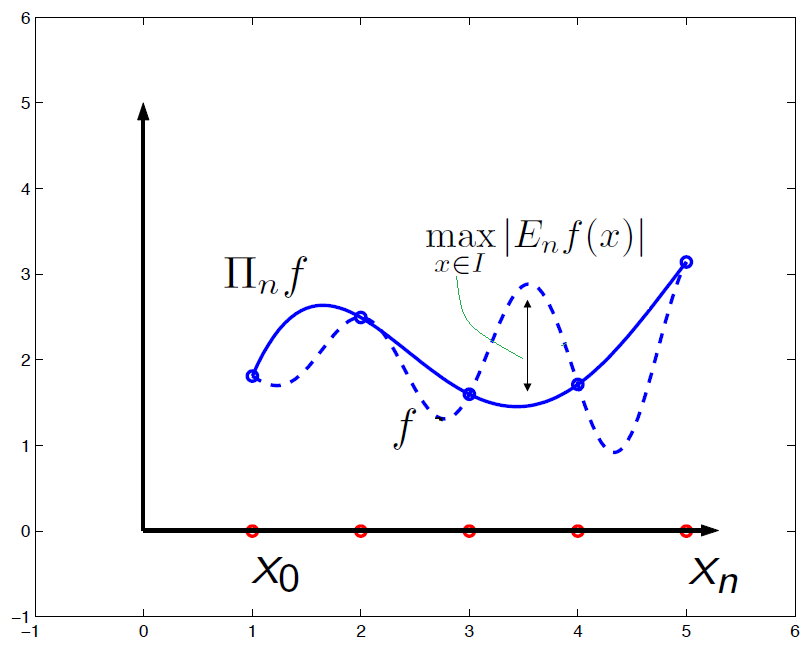
\includegraphics[width=0.55\textwidth]{ch3_max_error.png}
\caption{L'errore massimo di interpolazione \`e il massimo valore assoluto dell'errore puntuale sull'intero intervallo.}
\end{figure}

\section{Fenomeno di Runge}
L'interpolazione polinomiale globale su nodi equispaziati pu\`o non convergere quando il numero dei nodi aumenta. Questo comportamento prende il nome di \emph{fenomeno di Runge}: le oscillazioni dell'errore tendono a concentrarsi e ad amplificarsi vicino agli estremi dell'intervallo.

\begin{figure}[H]
\centering
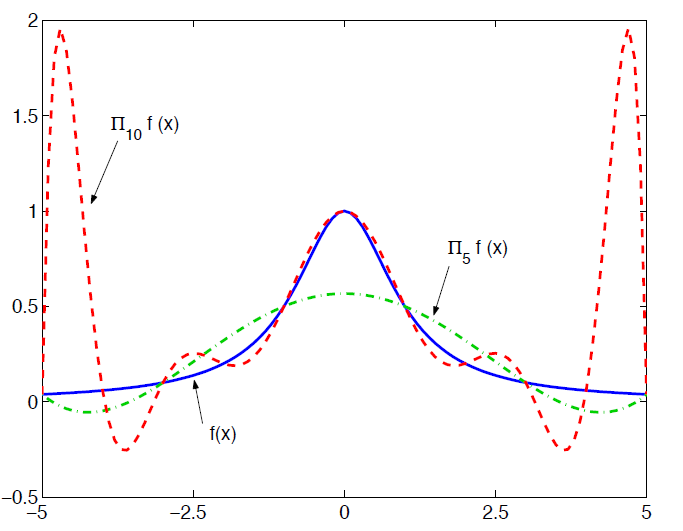
\includegraphics[width=0.62\textwidth]{ch3_runge.png}
\caption{Fenomeno di Runge per la funzione $f(x)=1/(1+x^2)$: aumentando il grado dell'interpolante globale sui nodi equispaziati, le oscillazioni agli estremi peggiorano.}
\end{figure}

\section{Interpolazione Lagrangiana composita}
Per evitare l'instabilit\`a dell'interpolazione globale di alto grado, una strategia consiste nel suddividere l'intervallo in sottointervalli e costruire in ciascuno un interpolatore di basso grado $k$ (tipicamente $k=1,2,3$). L'unione di questi interpolatori locali definisce un interpolatore composito continuo. Se i nodi sono equispaziati e $H=kh$ \`e la lunghezza di ciascun sottointervallo, l'idea \`e far crescere il numero degli intervalli senza aumentare il grado locale.

\begin{figure}[H]
\centering
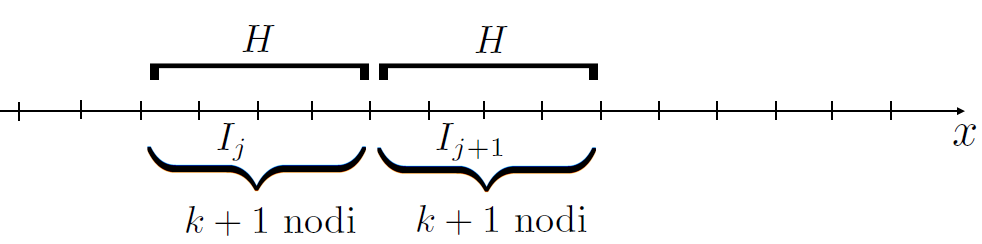
\includegraphics[width=0.68\textwidth]{ch3_composite_intervals.png}
\caption{Suddivisione del dominio in sottointervalli di ampiezza $H$, ciascuno contenente $k+1$ nodi.}
\end{figure}

Nel caso composito, l'errore globale coincide con il massimo degli errori locali. Nei lucidi si ottiene quindi una stima del tipo
\begin{formulaBox}
\[
 \max_{x\in I}|E^{H}_k f(x)|\le C\,H^{k+1},
\]
\end{formulaBox}
dove $C$ \`e una costante indipendente da $H$. Questo garantisce la convergenza dell'interpolazione composita al decrescere di $H$ e, lavorando con gradi locali piccoli, evita il fenomeno di Runge.

\begin{figure}[H]
\centering
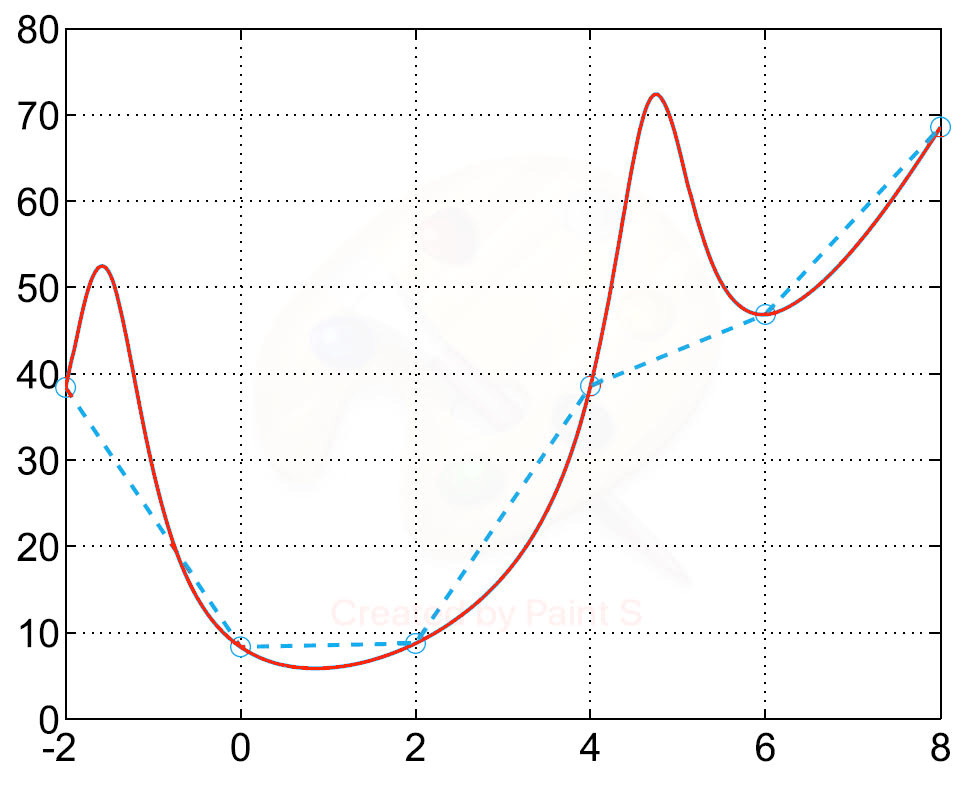
\includegraphics[width=0.68\textwidth]{ch3_composite_linear.png}
\caption{Esempio di interpolazione Lagrangiana composita lineare: l'approssimante globale \`e ottenuto incollando interpolanti locali di primo grado.}
\end{figure}

Nella pratica:
\begin{itemize}
  \item se la funzione $f$ \`e nota, si sceglie un grado locale piccolo e poi si determina $H$ in modo da rispettare l'accuratezza desiderata;
  \item se i dati provengono da misure, il numero dei nodi \`e fissato e si preferiscono in genere interpolazioni composite lineari o quadratiche.
\end{itemize}

\section{Ubicazione specifica dei nodi: nodi di Chebyshev}
Un'altra strategia per migliorare la stabilita consiste nel non usare nodi equispaziati, ma nodi collocati in posizioni speciali che si addensano verso gli estremi, cioe proprio nelle regioni in cui il fenomeno di Runge tende a manifestarsi. Sul dominio $[-1,1]$ si introducono i \emph{nodi di Chebyshev}
\begin{formulaBox}
\[
 \widehat x_j=-\cos\!\left(\frac{j\pi}{n}\right),
 \qquad j=0,\dots,n.
\]
\end{formulaBox}
Questi nodi si ottengono come proiezioni sull'asse $x$ di punti della semicirconferenza unitaria individuati da angoli equispaziati. Essi sono piu fitti vicino a $-1$ e $1$, e per questo sono molto piu stabili dei nodi equispaziati quando si costruisce un interpolatore polinomiale globale di alto grado.

\begin{figure}[H]
\centering
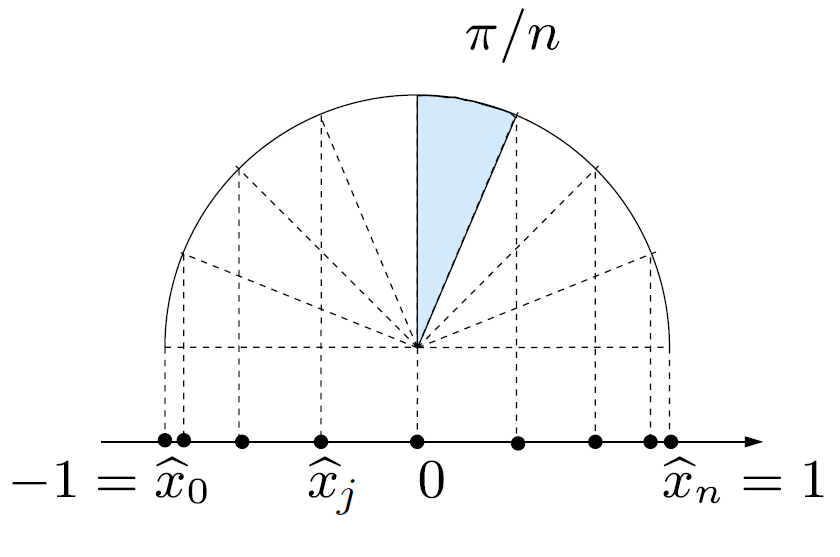
\includegraphics[width=0.70\textwidth]{ch3_chebyshev_nodes.png}
\caption{Nodi di Chebyshev su $[-1,1]$: la loro distribuzione mostra il tipico addensamento verso gli estremi dell'intervallo.}
\end{figure}

\subsection{Interpolatore sui nodi di Chebyshev}
Consideriamo ora l'interpolatore Lagrangiano di grado $n$ costruito sui nodi di Chebyshev. Questo viene costruito esattamente come nel caso generale, a patto di prendere come nodi su cui costruire i polinomi caratteristici di Lagrange le ascisse $\widehat x_j$. Si introducono quindi i corrispondenti polinomi caratteristici
\[
 \varphi_k^C(x)=\prod_{\substack{j=0 \\ j\ne k}}^n\frac{x-\widehat x_j}{\widehat x_k-\widehat x_j},
 \qquad k=0,\dots,n,
\]
e l'interpolatore Lagrangiano sui nodi di Chebyshev
\begin{formulaBox}
\[
 \Pi_n^C(x)=\sum_{j=0}^n y_j\,\varphi_j^C(x).
\]
\end{formulaBox}
Quando i dati sono ottenuti dalla valutazione di una funzione $f$, indicheremo l'interpolatore con $\Pi_n^C f$.

\begin{figure}[H]
\centering
\begin{subfigure}{0.48\textwidth}
  \centering
  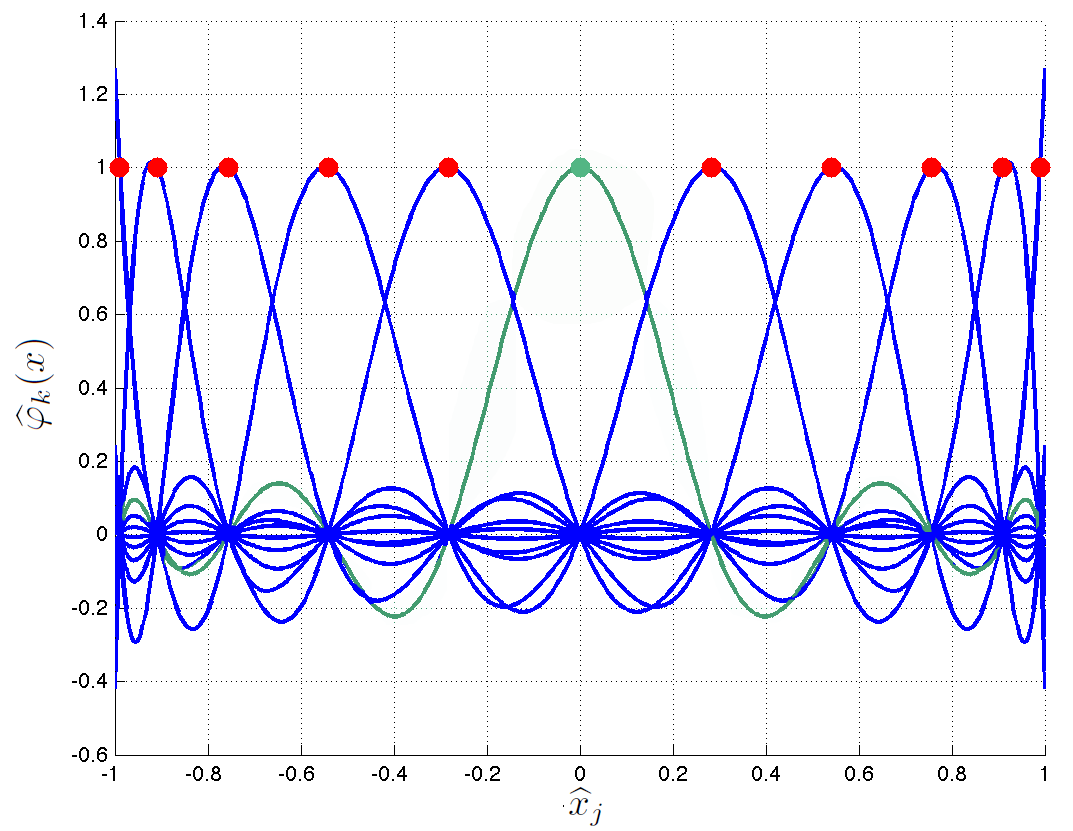
\includegraphics[width=\linewidth]{ch3_chebyshev_basis_compare.png}
  \caption{Polinomi caratteristici su nodi di Chebyshev.}
\end{subfigure}\hfill
\begin{subfigure}{0.48\textwidth}
  \centering
  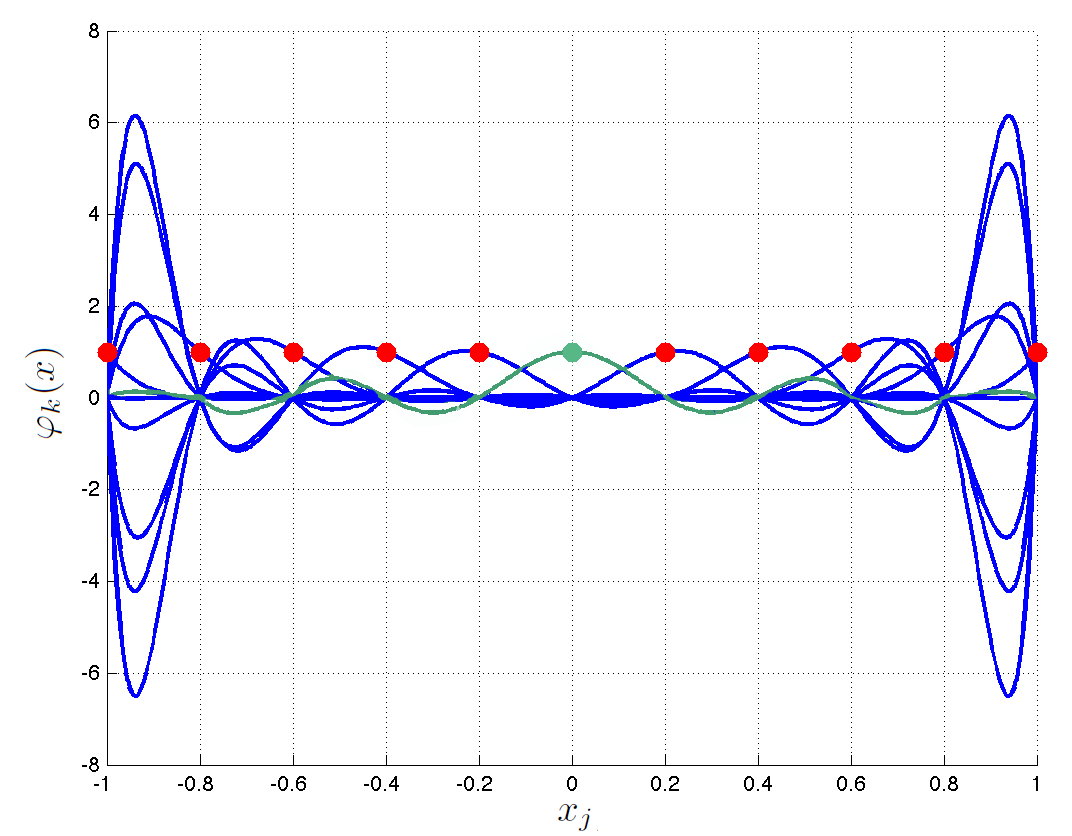
\includegraphics[width=\linewidth]{ch3_equispaced_basis_compare.png}
  \caption{Polinomi caratteristici su nodi equispaziati.}
\end{subfigure}
\caption{Confronto tra polinomi caratteristici sui nodi di Chebyshev e sui nodi equispaziati.}
\end{figure}

\section{Convergenza dell'interpolazione sui nodi di Chebyshev}
I lucidi riportano il seguente teorema. Supponiamo che la funzione ammetta derivata continua fino all'ordine $s+1$ compreso, ovvero
\[
 f\in C^{s+1}([-1,1]).
\]
Allora si ha il seguente risultato di convergenza:
\begin{formulaBox}
\[
 \max_{x\in[-1,1]}\big|f(x)-\Pi_n^C f(x)\big|\le C\,\frac{1}{n^s}
\]
\end{formulaBox}
per un'opportuna costante $C$.

Il precedente risultato ci dice che:
\begin{enumerate}[label=\roman*)]
  \item se $s>0$, allora si ha sempre convergenza, cio\`e
  \[
   \lim_{n\to\infty}\max_{x\in[-1,1]}\big|f(x)-\Pi_n^C f(x)\big|=0;
  \]
  \item la velocit\`a di convergenza \`e tanto pi\`u alta tanto pi\`u \`e alto $s$;
  \item se l'ipotesi del teorema vale per ogni $s>0$, tale velocit\`a \`e esponenziale, che \`e la stima migliore che si pu\`o ottenere, essendo pi\`u veloce di qualsiasi $1/n^s$.
\end{enumerate}

Per un intervallo generico $[a,b]$ si ottengono i nodi di Chebyshev tramite la mappa affine
\[
 x=\frac{a+b}{2}+\frac{b-a}{2}\,\widehat x,
\]
cioe
\begin{formulaBox}
\[
 x_j=\frac{a+b}{2}+\frac{b-a}{2}\,\widehat x_j,
 \qquad j=0,\dots,n.
\]
\end{formulaBox}
In questo modo seguono in maniera del tutto analoga al caso di dominio $[-1,1]$ la definizione dei polinomi caratteristici di Lagrange, dell'interpolatore Lagrangiano e delle sue propriet\`a di convergenza su un intervallo generico.

\begin{figure}[H]
\centering
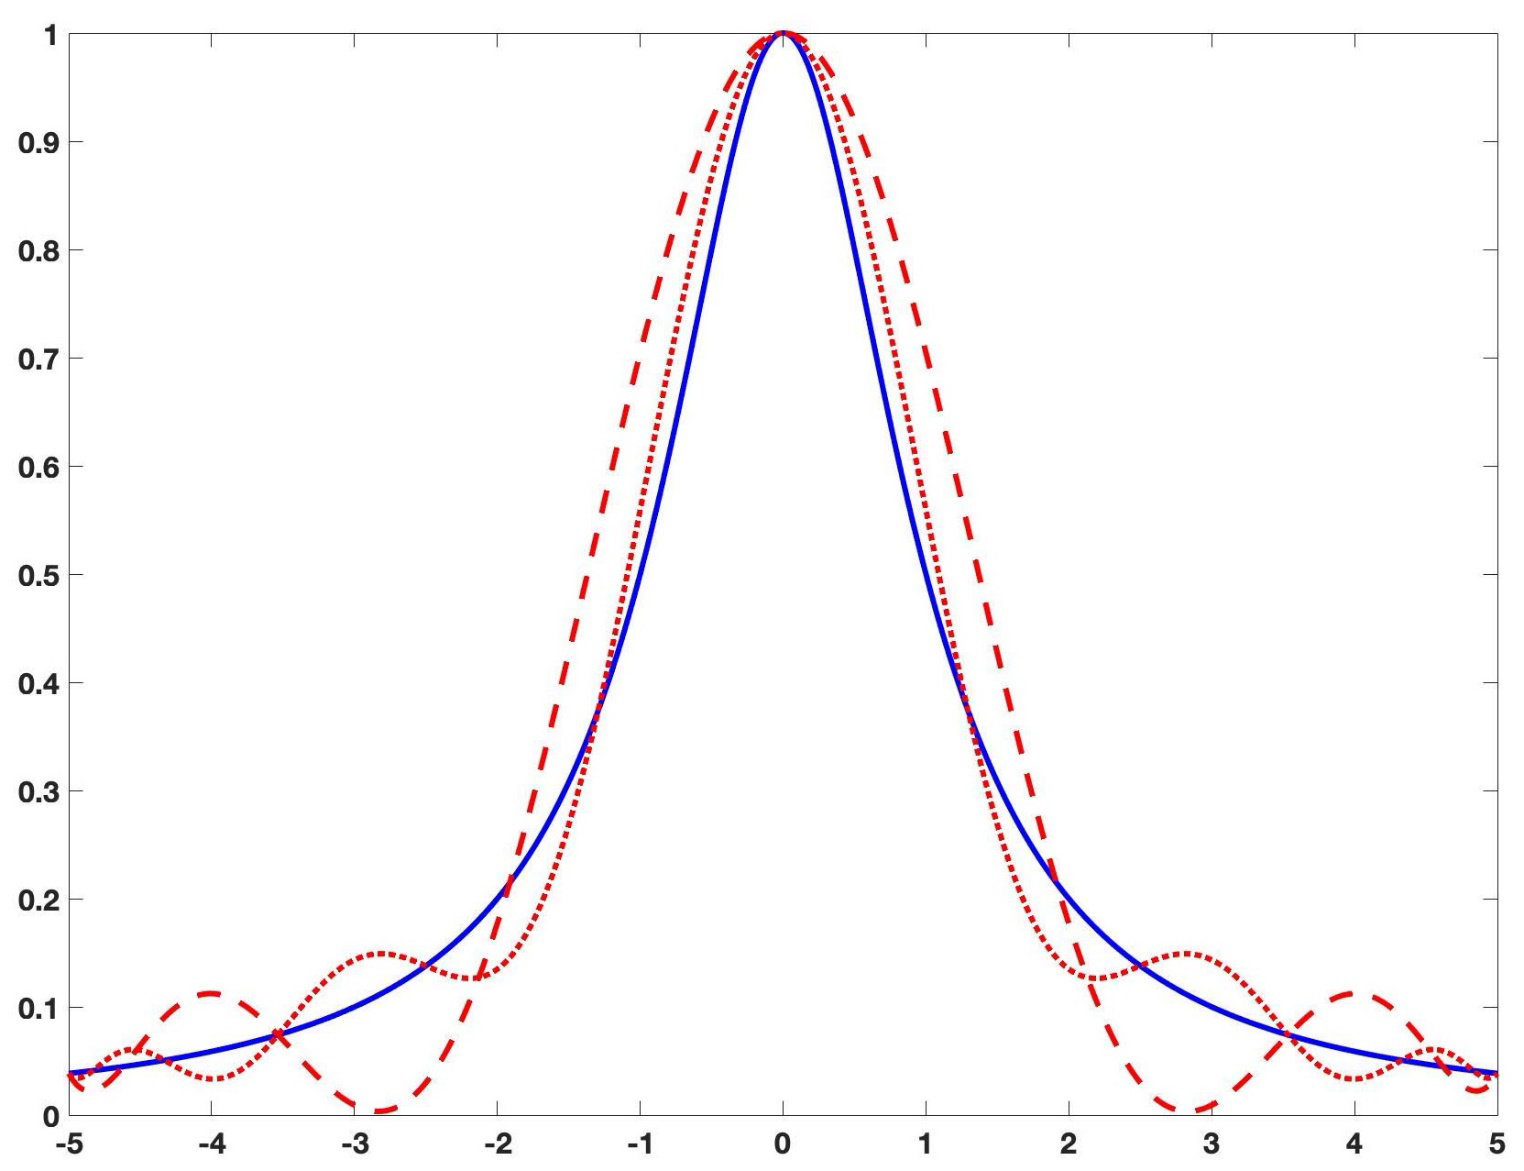
\includegraphics[width=0.74\textwidth]{ch3_runge_chebyshev_stable.png}
\caption{Interpolatori Lagrangiani sui nodi di Chebyshev di ordine 8 e 12 per la funzione di Runge.}
\end{figure}


\section{Metodo dei minimi quadrati}
\subsection{Perche servono i minimi quadrati}
Supponiamo al solito di conoscere $n+1$ coppie di dati $(x_i,y_i)$ e di cercare un'approssimante globale di basso grado $m\ll n$ su tutto l'intervallo $[a,b]$ che contiene i nodi.

Questo e il caso in cui si voglia fare una \emph{estrapolazione} dei dati a disposizione, cioe una previsione anche al di fuori dell'intervallo dei dati osservati. Nei lucidi viene proposto, ad esempio, il prezzo di un'azione osservato negli ultimi 30 mesi, con l'obiettivo di stimare il valore nel mese successivo.

\begin{figure}[H]
\centering
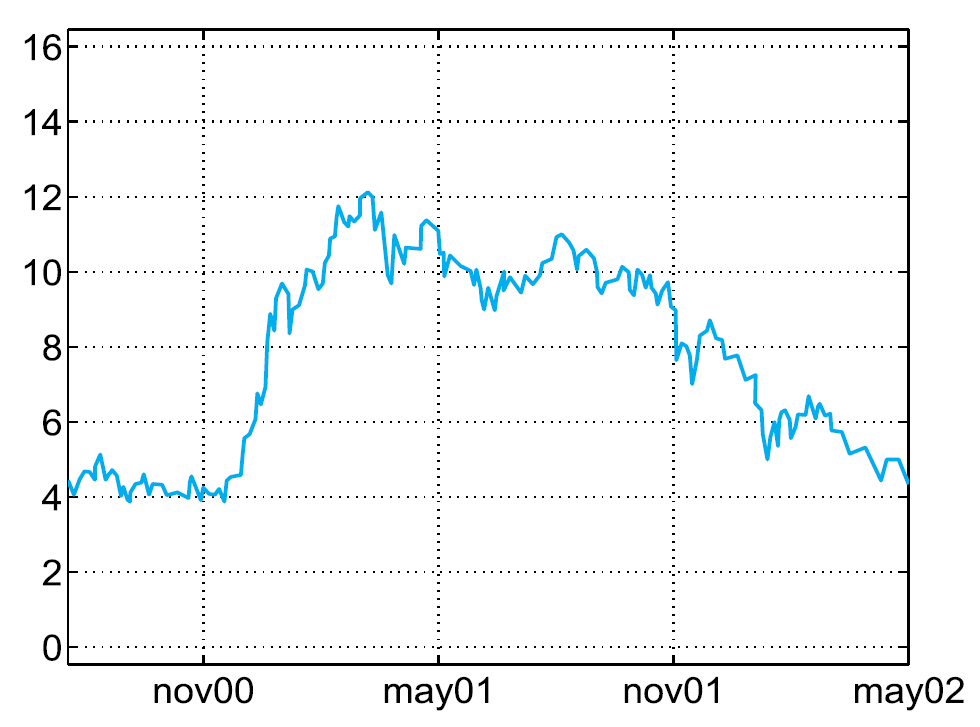
\includegraphics[width=0.72\textwidth]{ch3_finance_series.png}
\caption{Prezzo di un'azione negli ultimi 30 mesi.}
\end{figure}

Un altro ambito di interesse e la ricerca di una \emph{relazione analitica semplice} fra due quantita, ad esempio fra sforzo e deformazione nel caso del disco intervertebrale. In questi casi le strategie interpolatorie viste prima non sono adatte:
\begin{itemize}
  \item l'interpolazione Lagrangiana globale puo andare incontro al fenomeno di Runge se i dati sono numerosi;
  \item l'interpolazione composita usa solo blocchi locali di dati e non fornisce, in generale, una legge globale semplice;
  \item l'interpolazione sui nodi di Chebyshev non e in generale applicabile, perche i dati sperimentali sono assegnati e non posso scegliere liberamente i nodi.
\end{itemize}

Si cerca quindi un polinomio globale di basso grado $m\ll n$ e, per fare questo, si deve \emph{abbandonare il vincolo di interpolazione}.

\subsection{Formulazione del problema}
Introduciamo lo spazio dei polinomi di grado al piu $m$:
\[
\mathbb P_m = \{p_m(x)=b_0+b_1x+\dots+b_mx^m\}.
\]

Dato un polinomio $p_m\in\mathbb P_m$, l'errore nel nodo $x_i$ e dato da
\[
 e_i = y_i - p_m(x_i).
\]

L'idea dei minimi quadrati e cercare il polinomio di grado $m$ che minimizza la somma dei quadrati degli errori nei nodi. Si introduce quindi la funzione obiettivo
\begin{formulaBox}
\[
\Phi(b_0,\dots,b_m)=\sum_{i=0}^n [y_i-p_m(x_i)]^2.
\]
\end{formulaBox}
Il problema ai minimi quadrati consiste nel trovare i coefficienti del polinomio che realizzano il minimo di $\Phi$.

Nel caso generale, indicheremo con $(a_0,\dots,a_m)$ il vettore dei coefficienti del polinomio di miglior approssimazione nel senso dei minimi quadrati, cioe
\begin{formulaBox}
\[
(a_0,\dots,a_m):\qquad \Phi(a_0,\dots,a_m)=\min_{(b_0,\dots,b_m)}\Phi(b_0,\dots,b_m).
\]
\end{formulaBox}

Il quadrato viene usato per pesare nello stesso modo gli errori positivi e negativi e per penalizzare maggiormente gli scarti piu grandi.

\subsection{Retta di regressione}
Nel caso $m=1$ si parla di \emph{retta di regressione}. Il polinomio cercato ha la forma
\[
 p_1(x)=b_0+b_1x.
\]

La funzione da minimizzare diventa allora
\begin{formulaBox}
\[
\Phi(b_0,b_1)=\sum_{i=0}^n [y_i-p_m(x_i)]^2 = \sum_{i=0}^n [y_i-(b_0+b_1x_i)]^2.
\]
\end{formulaBox}

Il problema consiste nel determinare $(a_0,a_1)$ tali che
\begin{formulaBox}
\[
(a_0,a_1):\qquad \Phi(a_0,a_1)=\min_{(b_0,b_1)}\Phi(b_0,b_1).
\]
\end{formulaBox}

Svolgendo i quadrati si ottiene
\[
\Phi(b_0,b_1)=\sum_{i=0}^n y_i^2 + (n+1)b_0^2 + b_1^2\sum_{i=0}^n x_i^2
-2b_0\sum_{i=0}^n y_i -2b_1\sum_{i=0}^n x_i y_i + 2b_0b_1\sum_{i=0}^n x_i.
\]

Il punto di minimo si ottiene imponendo
\[
\frac{\partial \Phi}{\partial b_0}(b_0,b_1)=0,
\qquad
\frac{\partial \Phi}{\partial b_1}(b_0,b_1)=0.
\]

Queste condizioni portano al seguente sistema lineare in due equazioni e due incognite:
\begin{formulaBox}
\[
\left\{
\begin{aligned}
(n+1)b_0 + \left(\sum_{i=0}^n x_i\right)b_1 &= \sum_{i=0}^n y_i,\\
\left(\sum_{i=0}^n x_i\right)b_0 + \left(\sum_{i=0}^n x_i^2\right)b_1 &= \sum_{i=0}^n x_i y_i.
\end{aligned}
\right.
\]
\end{formulaBox}

Equivalentemente,
\[
 \begin{bmatrix}
 n+1 & \sum_{i=0}^n x_i\\
 \sum_{i=0}^n x_i & \sum_{i=0}^n x_i^2
 \end{bmatrix}
 \begin{bmatrix}
 b_0\\ b_1
 \end{bmatrix}
 =
 \begin{bmatrix}
 \sum_{i=0}^n y_i\\
 \sum_{i=0}^n x_i y_i
 \end{bmatrix}.
\]

Indicando con
\[
D=(n+1)\sum_{i=0}^n x_i^2 - \left(\sum_{i=0}^n x_i\right)^2,
\]
la soluzione del sistema e data da
\begin{formulaBox}
\[
 a_0=\frac{1}{D}\left[\left(\sum_{i=0}^n y_i\right)\left(\sum_{j=0}^n x_j^2\right)-\left(\sum_{j=0}^n x_j\right)\left(\sum_{i=0}^n x_i y_i\right)\right],
\]
\[
 a_1=\frac{1}{D}\left[(n+1)\sum_{i=0}^n x_i y_i - \left(\sum_{j=0}^n x_j\right)\left(\sum_{i=0}^n y_i\right)\right].
\]
\end{formulaBox}

Questi coefficienti individuano la retta di regressione
\[
 p_1(x)=a_0+a_1x.
\]

\begin{figure}[H]
\centering
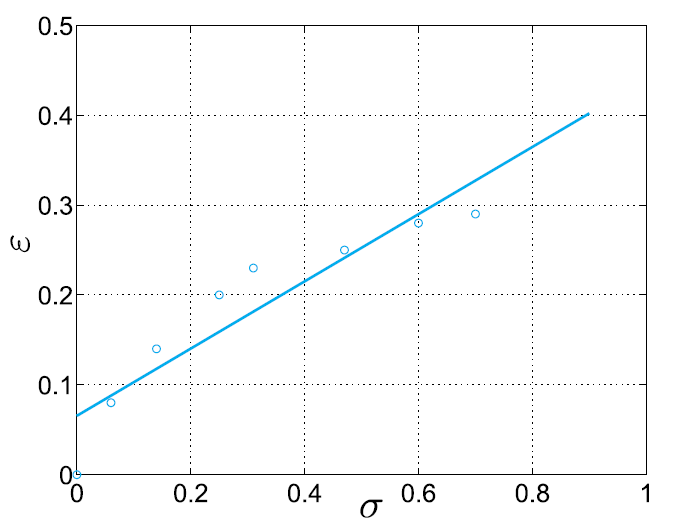
\includegraphics[width=0.58\textwidth]{ch3_regression_line_repeat.png}
\caption{Retta di regressione per i dati sforzo-deformazione del disco intervertebrale.}
\end{figure}

\subsection{Caso generale}
Nel caso di un polinomio di grado $m$, si scrive
\[
 p_m(x)=\sum_{j=0}^m b_j x^j.
\]

La funzione da minimizzare e
\[
\Phi(b_0,\dots,b_m)=\sum_{i=0}^n\left[y_i-\sum_{j=0}^m b_j x_i^j\right]^2.
\]

Per trovare gli $m+1$ coefficienti si impongono le condizioni di ottimalita
\[
\frac{\partial \Phi}{\partial b_k}(b_0,\dots,b_m)=0,
\qquad k=0,\dots,m.
\]

Si ottiene cosi il seguente sistema lineare in $m+1$ equazioni e $m+1$ incognite:
\begin{formulaBox}
\[
\sum_{j=0}^m\left(\sum_{i=0}^n x_i^{j+k}\right)b_j = \sum_{i=0}^n y_i x_i^k,
\qquad k=0,\dots,m.
\]
\end{formulaBox}

Il problema dei minimi quadrati si riconduce quindi ancora alla risoluzione di un sistema lineare. Nel caso limite $m=n$, si ritrova l'interpolazione polinomiale.

\begin{figure}[H]
\centering
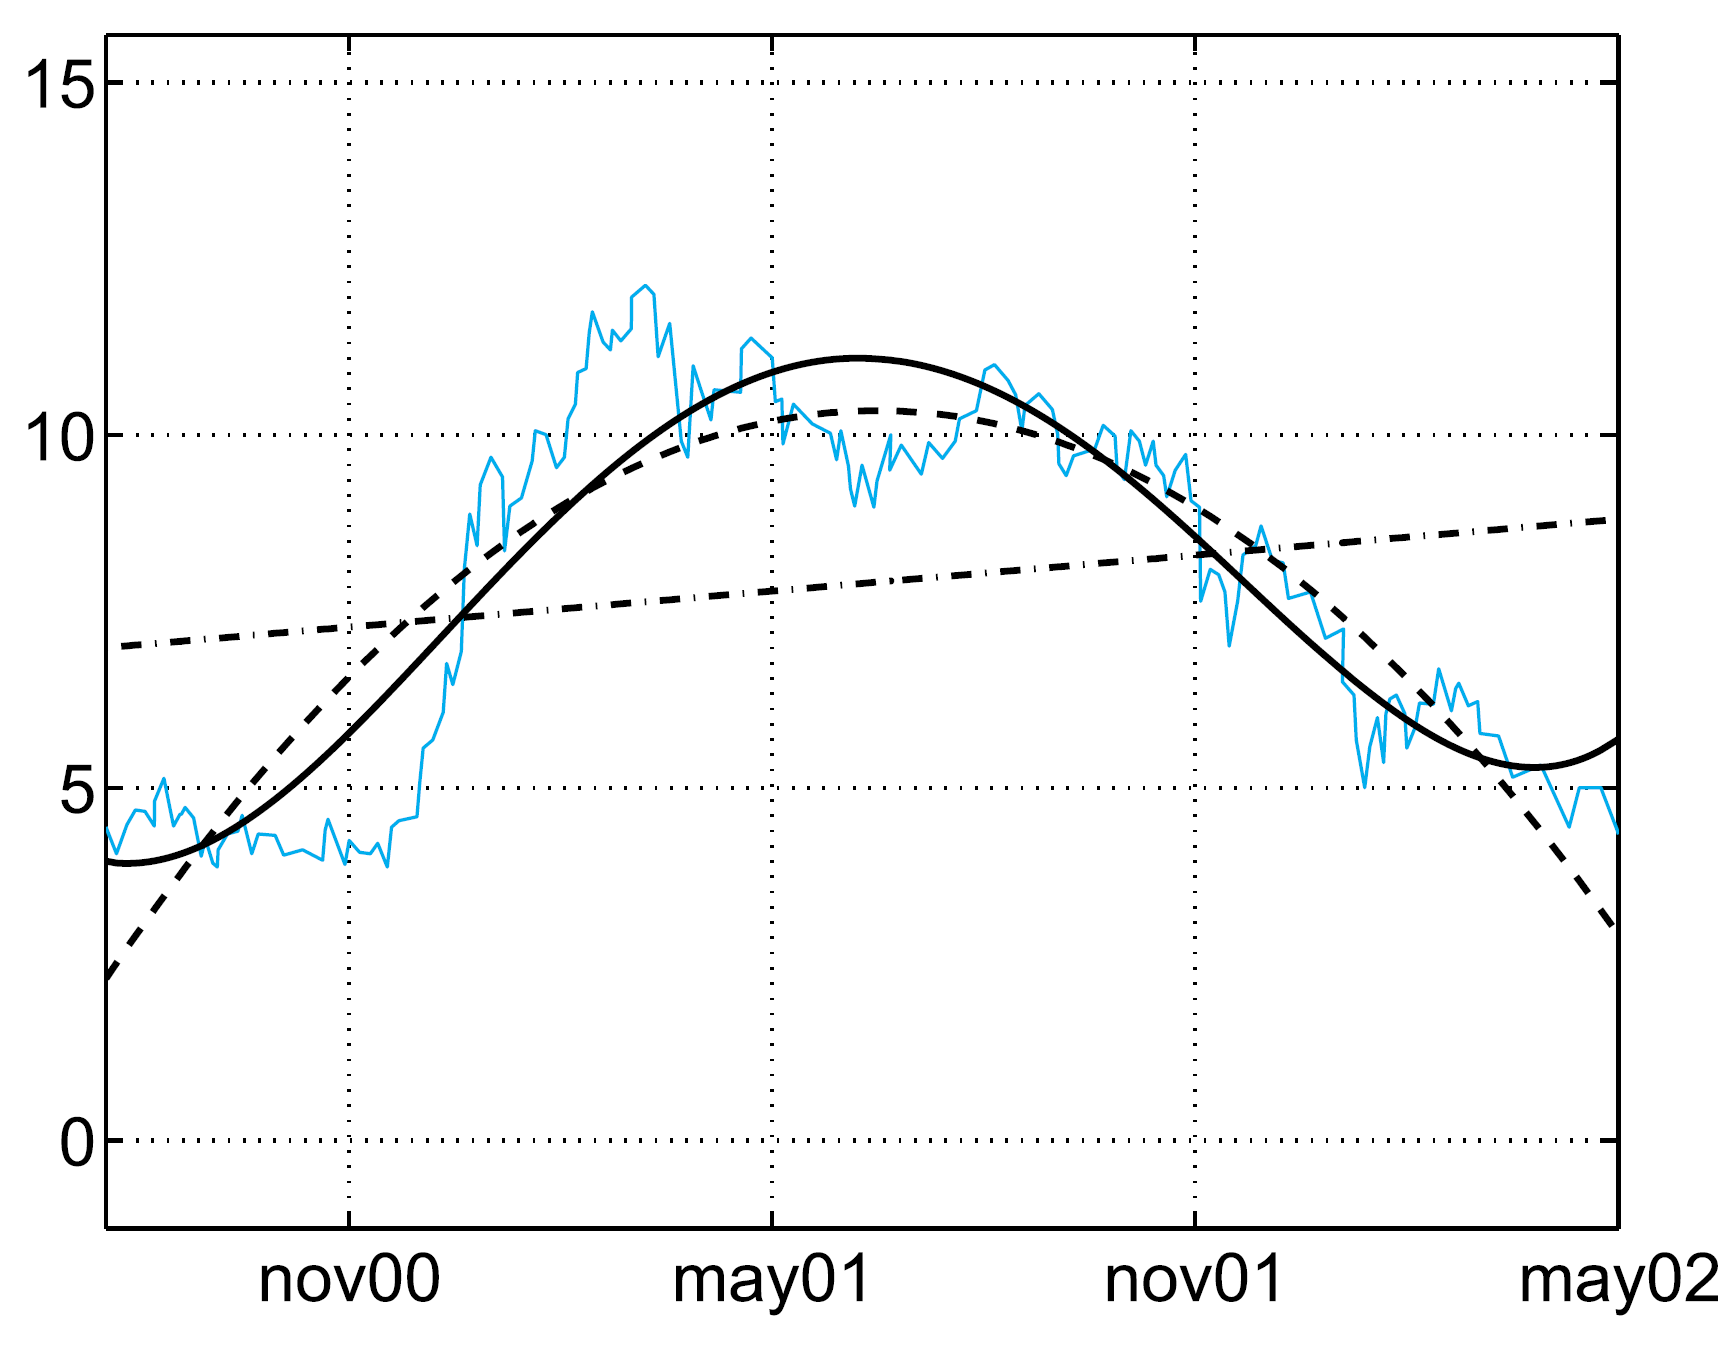
\includegraphics[width=0.84\textwidth]{ch3_finance_least_squares_models.png}
\caption{Approssimazioni ai minimi quadrati per il problema di finanza con $m=1$, $m=2$ e $m=4$.}
\end{figure}




\chapter{Integrazione numerica}

\section{Esempio introduttivo}
Consideriamo l'altezza degli $M$ individui di una popolazione.
La sua distribuzione $n(s)$ pu\`o essere rappresentata da
\begin{formulaBox}
\[
 n(s)=\frac{M}{\sigma\sqrt{2\pi}}e^{-(s-\bar h)^2/(2\sigma^2)},
\]
\[
 \sigma=\sqrt{\frac{\sum_i (h_i-\bar h)^2}{N}},
\]
\end{formulaBox}
dove $\bar h$ \`e il valor medio, $\sigma$ la deviazione standard e $h_i$ gli $N$ campioni usati.

Il valore degli individui che hanno un'altezza compresa fra $h$ e $h+\Delta h$ \`e dato dal seguente integrale:
\begin{formulaBox}
\[
 N_{[h,h+\Delta h]}=\int_h^{h+\Delta h} n(s)\,ds.
\]
\end{formulaBox}

Non conoscendo in generale la primitiva di $n(s)$, non sappiamo calcolare esattamente questo integrale.
Tale valore \`e dato dall'area sottesa alla curva $n(s)$ e compresa fra i valori $h$ e $h+\Delta h$.

\begin{figure}[H]
\centering
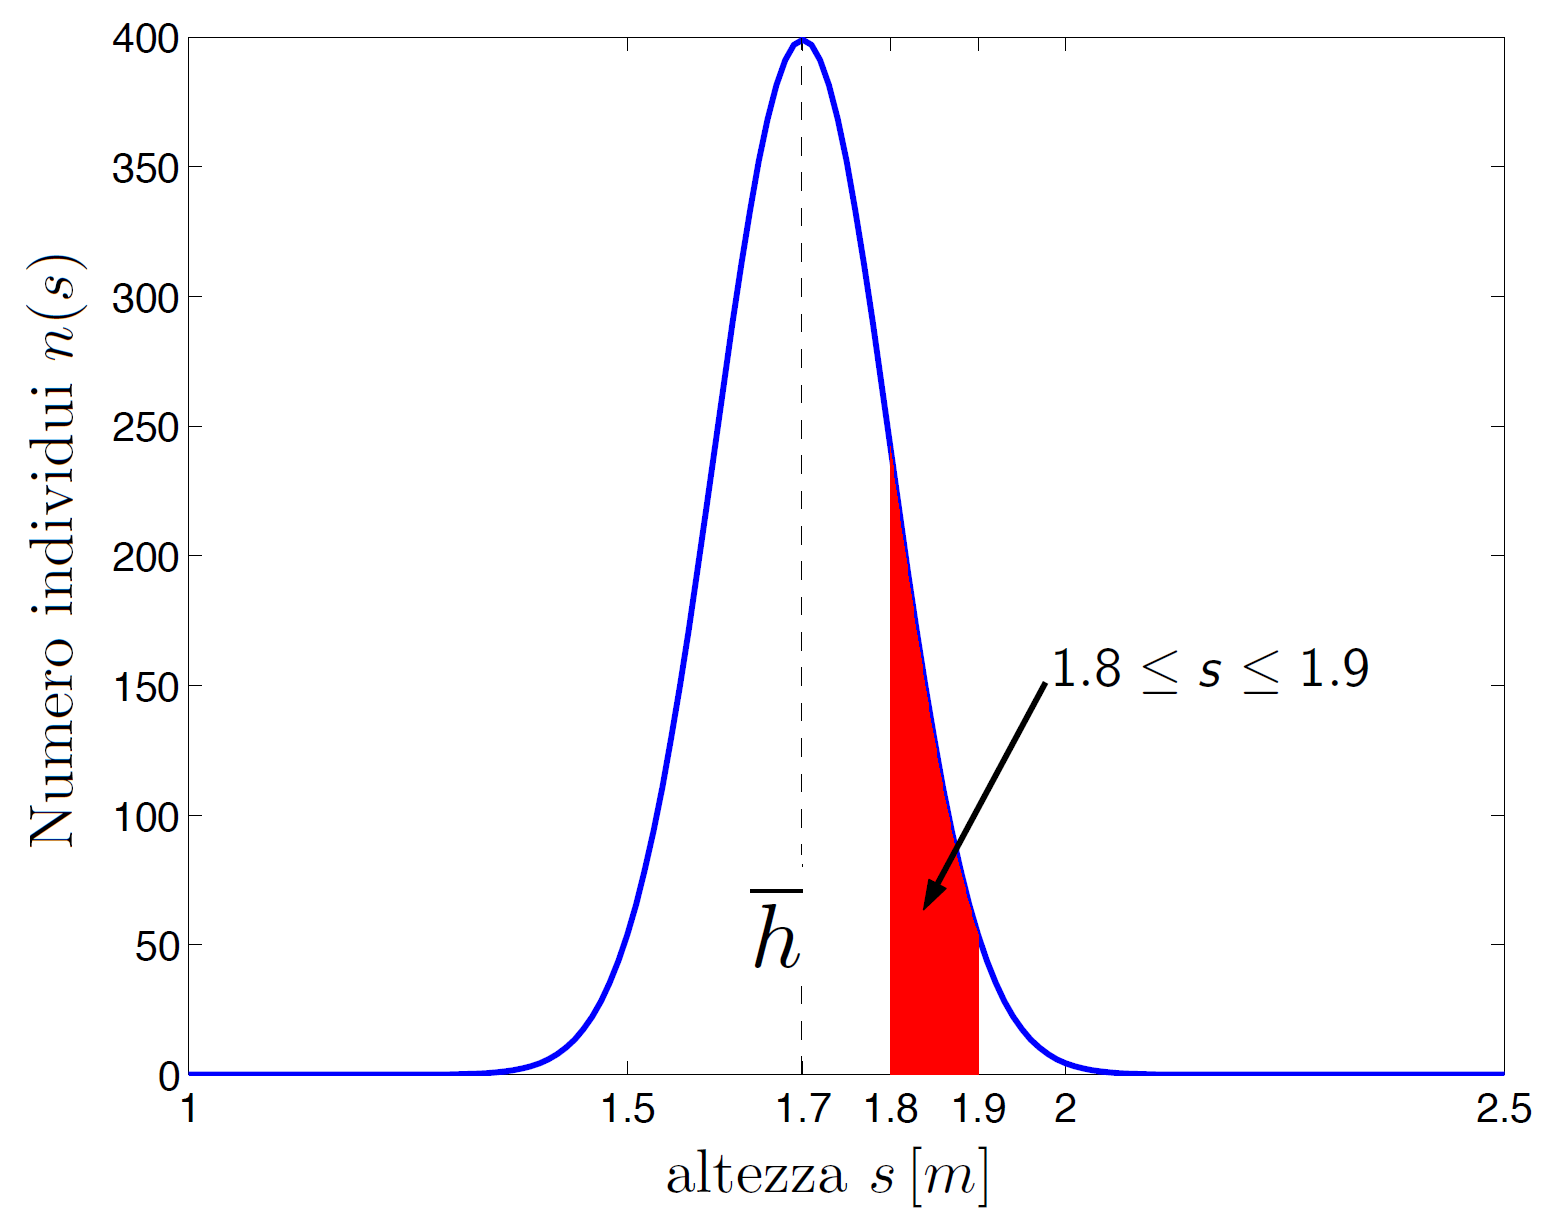
\includegraphics[width=0.73\textwidth]{ch4_population_band.png}
\caption{Numero di individui con altezza compresa fra $1.8$ e $1.9$. L'area rossa rappresenta il valore dell'integrale su quell'intervallo.}
\end{figure}

\section{Formule di quadratura composite}

\subsection{Notazione}
Consideriamo l'integrale
\begin{formulaBox}
\[
 I(f)=\int_a^b f(x)\,dx.
\]
\end{formulaBox}

Suddividiamo l'intervallo $[a,b]$ in $M$ intervalli $I_k$ di ampiezza costante $H$:
\[
 I_k=[x_{k-1},x_k], \qquad k=1,\dots,M,
\]
\[
 x_k=a+kH, \qquad k=0,\dots,M.
\]
Introduciamo inoltre su ogni intervallo i punti medi
\[
 \bar x_k=\frac{x_{k-1}+x_k}{2}.
\]

\begin{figure}[H]
\centering
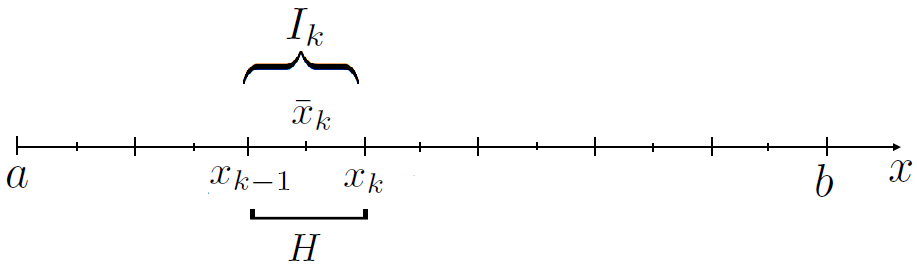
\includegraphics[width=0.78\textwidth]{ch4_interval_notation.png}
\caption{Suddivisione di $[a,b]$ in intervalli $I_k$ di ampiezza $H$ e corrispondenti punti medi $\bar x_k$.}
\end{figure}

\subsection{Definizioni}
Consideriamo una formula di quadratura per il calcolo approssimato di $I(f)$ e sia $I_H(f)$ il valore approssimato ottenuto.

Si dice che la formula di quadratura \`e di \emph{ordine $p$} se l'errore soddisfa la seguente stima:
\begin{formulaBox}
\[
 E_H=\abs{I(f)-I_H(f)}\le CH^p.
\]
\end{formulaBox}

Si dice inoltre che la formula di quadratura ha \emph{grado di esattezza} pari ad $r$ se essa risulta esatta quando applicata ai polinomi di grado minore o uguale ad $r$, cio\`e se
\begin{formulaBox}
\[
 E_H=\abs{I(f)-I_H(f)}=0 \qquad \forall f\in \mathbb P^r(a,b).
\]
\end{formulaBox}

\section{Formula del punto medio composita}
Partiamo dalla propriet\`a di additivit\`a dell'integrale, cio\`e
\[
 I(f)=\sum_{k=1}^M \int_{I_k} f(x)\,dx.
\]

L'idea della formula del punto medio composita si basa sull'approssimare il valore di $\int_{I_k} f(x)\,dx$ con l'area del rettangolo che ha per altezza $f(\bar x_k)$.
Poich\'e la base di questi rettangoli \`e sempre pari ad $H$, avremo quindi la seguente approssimazione per $I(f)$:
\begin{formulaBox}
\[
 I_{pm}(f)=H\sum_{k=1}^M f(\bar x_k).
\]
\end{formulaBox}

\begin{figure}[H]
\centering
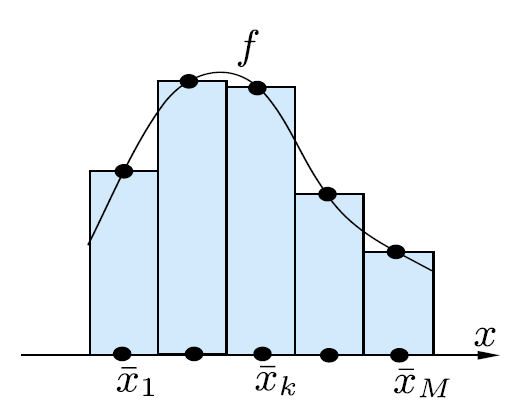
\includegraphics[width=0.36\textwidth]{ch4_midpoint_histogram.png}
\caption{Formula del punto medio composita: l'integrale viene approssimato con la somma delle aree dei rettangoli di altezza $f(\bar x_k)$.}
\end{figure}

% [BOX ROSSO NEI LUCIDI -- NON RICHIESTO ALL'ESAME]
\begin{nonExamBox}
Utilizzando lo sviluppo in serie di Taylor e assumendo che $f$ abbia derivata seconda continua, abbiamo che l'errore commesso su ogni intervallo $I_k$ vale:
\[
\int_{I_k} f(x)\,dx-Hf(\bar x_k)=\int_{I_k}(f(x)-f(\bar x_k))\,dx=
\]
\[
=\int_{I_k} f'(\bar x_k)(x-\bar x_k)\,dx+\frac12\int_{I_k} f''(\eta^k(x))(x-\bar x_k)^2\,dx,
\]
per un opportuno $\eta^k$ in $I_k$ che dipende da $x$.

Il primo integrale \`e nullo perch\'e $f'(\bar x_k)$ \`e costante e
\[
 \int_{I_k}(x-\bar x_k)\,dx=0.
\]

Grazie al teorema della media integrale, per il secondo integrale esiste un opportuno $\xi^k$ in $I_k$ tale per cui
\[
 \frac12\int_{I_k} f''(\eta^k(x))(x-\bar x_k)^2\,dx=
 \frac12 f''(\xi^k)\int_{I_k}(x-\bar x_k)^2\,dx.
\]

Risolvendo analiticamente il secondo integrale, si ottiene
\[
 \frac12 f''(\xi^k)\int_{I_k}(x-\bar x_k)^2\,dx=
 \frac12 f''(\xi^k)\left[\frac{(x-\bar x_k)^3}{3}\right]_{x_{k-1}}^{x_k}
 =\frac{H^3}{24}f''(\xi^k).
\]

Sommando su ogni intervallo si ottiene:
\[
 \abs{I(f)-I_{pm}(f)}=\left|\sum_{k=1}^M\left(\int_{I_k}f(x)\,dx-Hf(\bar x_k)\right)\right|
 =\left|\sum_{k=1}^M \frac{H^3}{24}f''(\xi^k)\right|
\]
\[
 \le \max_k \abs{f''(\xi^k)}\,\frac{H^2}{24}\sum_{k=1}^M H.
\]
\end{nonExamBox}

Da cui, prendendo il massimo su tutto $(a,b)$, segue la seguente stima dell'errore:
\begin{formulaBox}
\[
 \abs{I(f)-I_{pm}(f)}\le \max_x \abs{f''(x)}\,\frac{b-a}{24}H^2.
\]
\end{formulaBox}

Dalla precedente stima si evince che:
\begin{itemize}
  \item la formula del punto medio composita \`e di ordine $2$;
  \item la formula del punto medio composita ha grado di esattezza pari a $1$.
\end{itemize}
Infatti, ricordando che stiamo assumendo $f$ con derivata seconda continua, si ha che $f''=0$ in ogni $x$ se $f$ \`e una retta, cio\`e per $r=1$.

\begin{figure}[H]
\centering
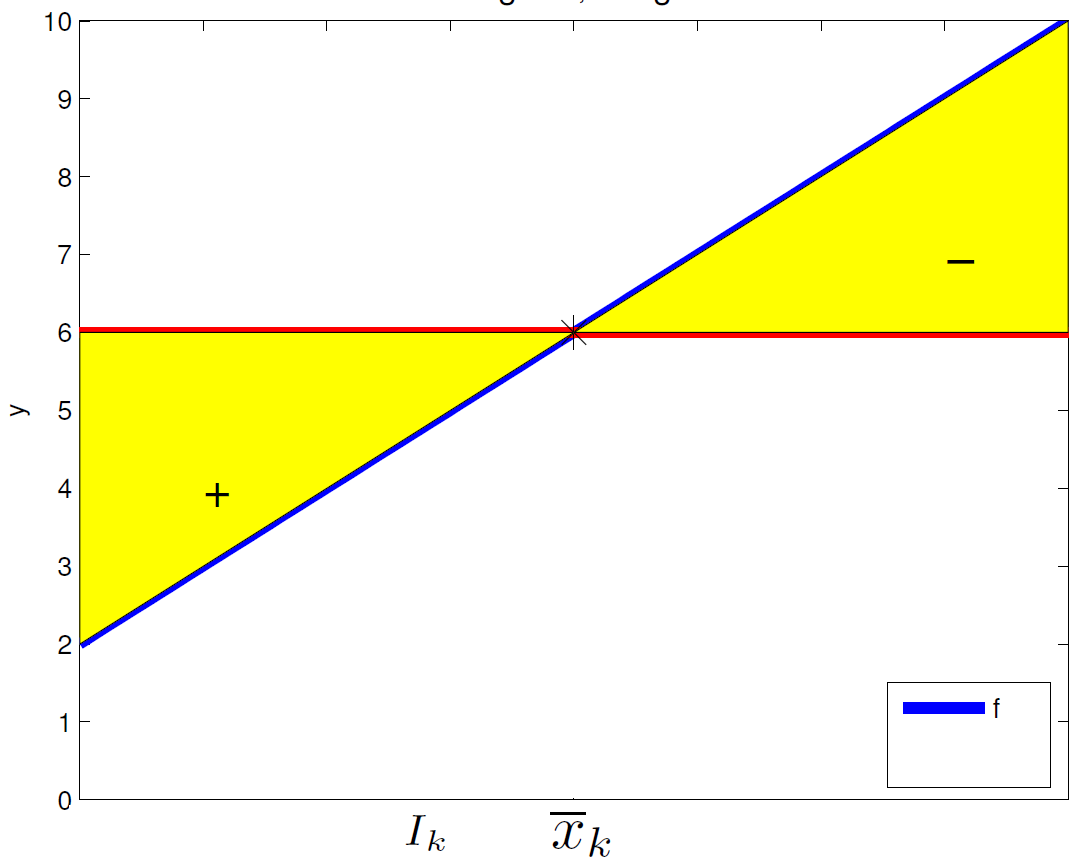
\includegraphics[width=0.62\textwidth]{ch4_midpoint_exactness_line.png}
\caption{Rappresentazione grafica del fatto che la formula del punto medio composita \`e esatta sulle rette: gli errori sui singoli intervalli si elidono a vicenda.}
\end{figure}

\section{Formula dei trapezi composita}
Partiamo sempre dalla propriet\`a di additivit\`a dell'integrale. Questa volta approssimiamo l'area sottesa da $f$ nell'intervallo $I_k$ considerando il trapezio costruito sui punti $x_{k-1}$ e $x_k$ e sulle corrispondenti ordinate.

Si ha quindi la formula dei trapezi composita:
\begin{formulaBox}
\[
 I_{tr}(f)=\frac{H}{2}\sum_{k=1}^M \big(f(x_{k-1})+f(x_k)\big).
\]
\end{formulaBox}

Per comodit\`a di implementazione, si scrive:
\[
 I_{tr}(f)=\frac{H}{2}\big(f(a)+f(b)\big)+H\sum_{k=1}^{M-1}f(x_k).
\]

\begin{figure}[H]
\centering
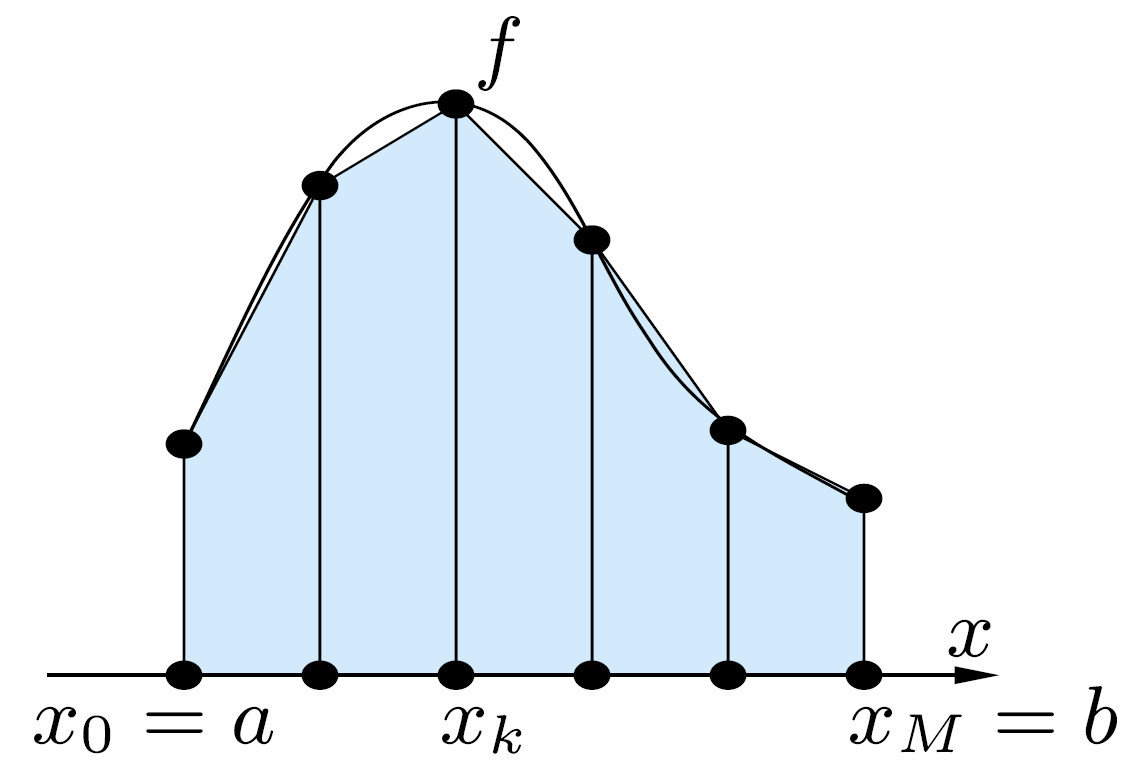
\includegraphics[width=0.36\textwidth]{ch4_trapezoid_composite.png}
\caption{Formula dei trapezi composita. Su ciascun intervallo l'area viene approssimata con l'area del trapezio determinato dagli estremi.}
\end{figure}

Notiamo che la formula dei trapezi composita equivale all'integrale esatto dell'interpolatore Lagrangiano composito di grado $1$:
\begin{formulaBox}
\[
 I_{tr}(f)=\int_a^b \Pi_1^H f(x)\,dx.
\]
\end{formulaBox}

Su ogni intervallo $I_k$ possiamo quindi considerare l'errore di interpolazione Lagrangiana. Relativamente all'espressione generale (si veda slide 20, Cap. 3), in questo caso abbiamo $k=1$, $x_0=x_{k-1}$ e $x_1=x_k$:
\[
 f(x)|_{I_k}-\Pi_1^H f(x)|_{I_k}=\frac{f''(\xi_x^k)}{2}(x-x_{k-1})(x-x_k).
\]


% [BOX ROSSO NEI LUCIDI -- NON RICHIESTO ALL'ESAME]
\begin{nonExamBox}
Quindi, l'errore commesso dalla formula dei trapezi composita su ogni intervallo $I_k$ vale:
\[
 I(f)|_{I_k}-I_{tr}(f)|_{I_k}=\int_{x_{k-1}}^{x_k}\big(f(x)-\Pi_1^H f(x)\big)=
\]
\[
=-\int_{x_{k-1}}^{x_k}\frac{f''(\xi_x^k)}{2}(x-x_{k-1})(x_k-x)\,dx.
\]

Procedendo in maniera analoga al caso del punto medio, grazie al teorema della media integrale, otteniamo, per un opportuno $\eta^k$:
\[
 I(f)|_{I_k}-I_{tr}(f)|_{I_k}=-\frac{f''(\eta^k)}{2}\int_{x_{k-1}}^{x_k}(x-x_{k-1})(x_k-x)\,dx
\]
\[
=-\frac{f''(\eta^k)}{12}H^3.
\]

Sommando ora questi contributi di errore su ogni intervallo $I_k$, otteniamo
\[
 \abs{I(f)-I_{tr}(f)}=\left|\sum_{k=1}^M \frac{f''(\eta^k)}{12}H^3\right|.
\]
\end{nonExamBox}

Da cui si ottiene la seguente stima dell'errore per la formula dei trapezi composita:
\begin{formulaBox}
\[
 \abs{I(f)-I_{tr}(f)}\le \frac{1}{12}\max_x \abs{f''(x)}\,(b-a)H^2.
\]
\end{formulaBox}

Dalla precedente si evince che:
\begin{itemize}
  \item la formula dei trapezi composita \`e di ordine $2$;
  \item la formula dei trapezi composita ha grado di esattezza pari a $1$.
\end{itemize}
Quindi ordine e grado di esattezza sono uguali a quelli del punto medio. La scelta di uno o dell'altro metodo risiede principalmente sull'avere a disposizione le coordinate dei punti medi o dei punti estremi degli intervalli.

\section{Formula di Simpson composita}
Partiamo sempre dalla propriet\`a di additivit\`a dell'integrale. Questa volta approssimiamo l'area sottesa da $f$ nell'intervallo $I_k$ considerando l'area sottesa dalla parabola che interpola i punti $x_{k-1}$, $\bar x_k$ e $x_k$.

Integrando esattamente tali parabole su ogni intervallo $I_k$, si ottiene la formula di Simpson composita:
\begin{formulaBox}
\[
 I_{sim}(f)=\frac{H}{6}\sum_{k=1}^M \big(f(x_{k-1})+4f(\bar x_k)+f(x_k)\big).
\]
\end{formulaBox}

\begin{figure}[H]
\centering
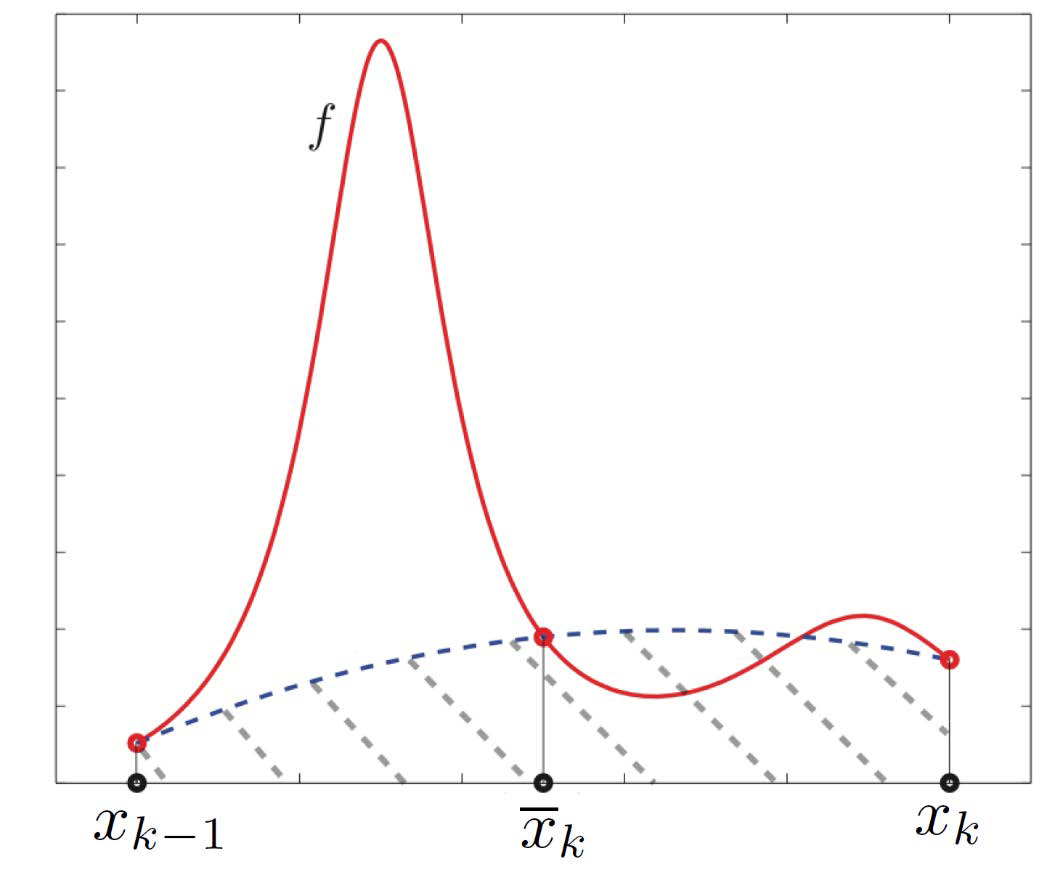
\includegraphics[width=0.66\textwidth]{ch4_simpson_parabola.png}
\caption{Formula di Simpson composita: su ogni intervallo si integra esattamente la parabola interpolante nei punti $x_{k-1}$, $\bar x_k$ e $x_k$.}
\end{figure}

Notiamo che per costruzione la formula di Simpson composita equivale all'integrale esatto dell'interpolatore Lagrangiano composito di grado $2$:
\begin{formulaBox}
\[
 I_{sim}(f)=\int_a^b \Pi_2^H f(x)\,dx.
\]
\end{formulaBox}

Si pu\`o mostrare che in questo caso vale il seguente risultato per l'errore, assumendo che $f$ abbia derivata quarta continua su $[a,b]$:
\begin{formulaBox}
\[
 \abs{I(f)-I_{sim}(f)}\le \frac{b-a}{2880}\max_x \abs{f^{(iv)}(x)}\,H^4.
\]
\end{formulaBox}

Dalla precedente uguaglianza si evince che:
\begin{itemize}
  \item la formula di Simpson composita \`e di ordine $4$;
  \item la formula di Simpson composita ha grado di esattezza pari a $3$.
\end{itemize}
Tale formula quindi non integra esattamente soltanto i polinomi che sono globalmente di grado $r=1$ (rette) e grado $r=2$ (parabole), ma anche i polinomi che sono globalmente di grado $3$ (cubiche).

\begin{figure}[H]
\centering
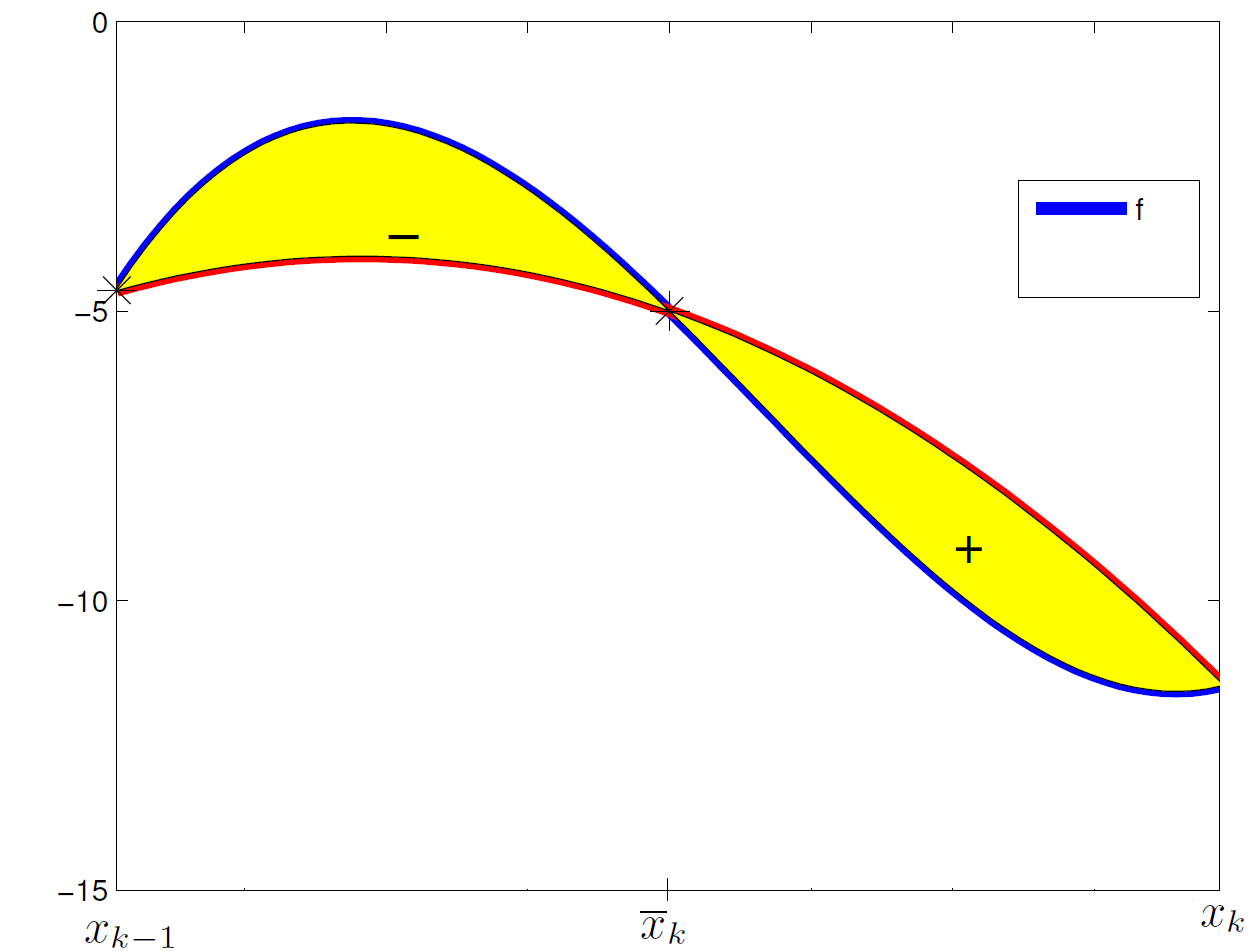
\includegraphics[width=0.74\textwidth]{ch4_simpson_cubic_exactness2.png}
\caption{Rappresentazione grafica del fatto che la formula di Simpson composita \`e esatta anche sulle cubiche: gli errori commessi sui singoli intervalli si elidono.}
\end{figure}

\section{Ricapitolando}
Ricapitolando abbiamo:

\begin{figure}[H]
\centering
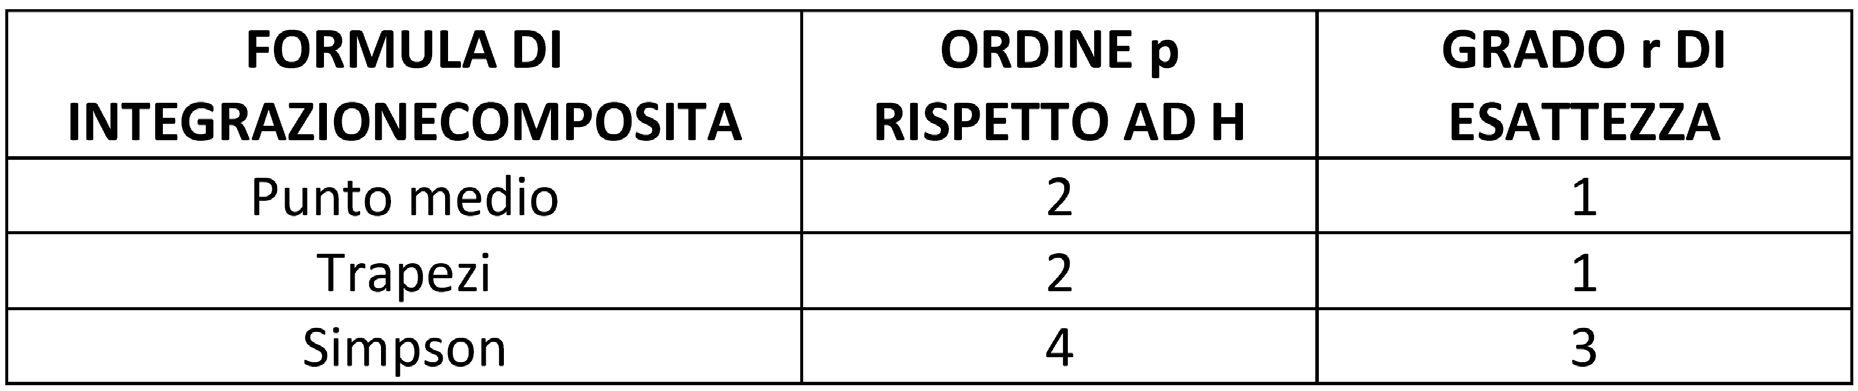
\includegraphics[width=0.92\textwidth]{ch4_summary_table.png}
\caption{Confronto fra formula del punto medio, formula dei trapezi e formula di Simpson: ordine rispetto ad $H$ e grado di esattezza.}
\end{figure}

\begin{figure}[H]
\centering
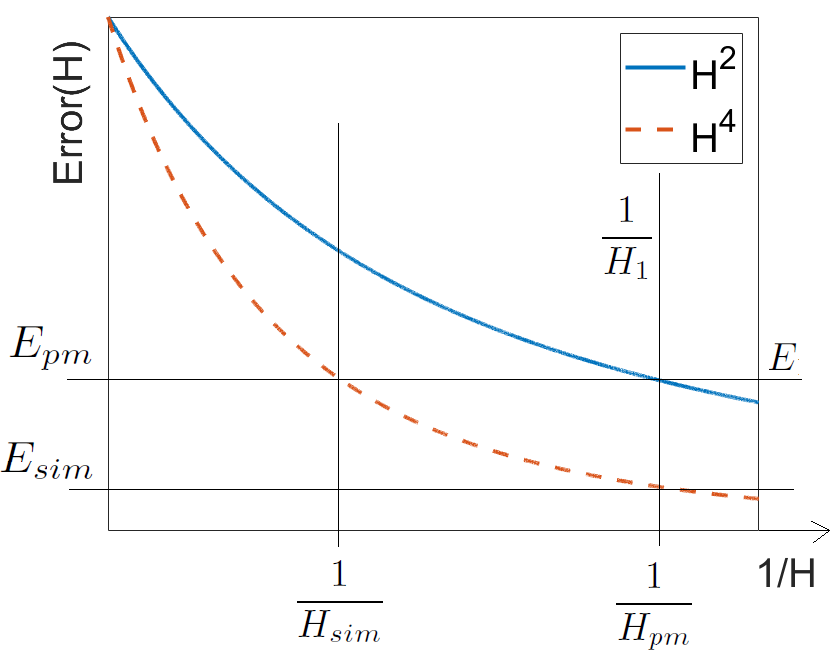
\includegraphics[width=0.75\textwidth]{ch4_summary_error_vs_H.png}
\caption{Per $H=H_1$ fissato, l'errore $E_{pm}$ del punto medio \`e maggiore dell'errore $E_{sim}$ di Simpson. Per scendere sotto una stessa soglia $E$, Simpson richiede un valore $H_{sim}$ maggiore del corrispondente $H_{pm}$ (equivalentemente $1/H_{sim}<1/H_{pm}$).}
\end{figure}

\chapter{Approssimazione numerica di equazioni differenziali ordinarie}

\section{Esempi introduttivi}
\subsection{Circuiti RC, RL e RLC}
Nei circuiti elettrici si ottengono naturalmente problemi di Cauchy del prim'ordine. Per i circuiti RC e RL si hanno, rispettivamente,
\[
\frac{dv_C(t)}{dt}+\frac{1}{RC}v_C(t)=\frac{1}{RC}V_s(t),
\qquad
\frac{di(t)}{dt}+\frac{R}{L}i(t)=\frac{V_s(t)}{L}.
\]
Nel caso RLC si ottiene invece il sistema
\[
\frac{d}{dt}V_C(t)=\frac{1}{C}i(t),
\qquad
\frac{d}{dt}i(t)=-\frac{1}{L}V_C(t)-\frac{R}{L}i(t)+\frac{1}{L}u(t).
\]
Questi esempi mostrano che molti problemi applicativi conducono naturalmente ad equazioni differenziali ordinarie.

\subsection{Modello preda-predatore}
Consideriamo due popolazioni in competizione fra loro, ad esempio volpi e conigli. Allora il numero di individui delle due popolazioni $y_1$ e $y_2$ \`e determinato dalle equazioni di Lotka--Volterra
\[
\frac{dy_1}{dt}=C_1y_1\bigl(1-b_1y_1-d_2y_2\bigr),
\qquad
\frac{dy_2}{dt}=-C_2y_2\bigl(1-b_2y_2-d_1y_1\bigr).
\]
Il precedente \`e un sistema di due equazioni differenziali ordinarie, la cui soluzione d\`a il numero di individui $y_1(t)$ e $y_2(t)$ al tempo $t$.

\begin{figure}[H]
\centering
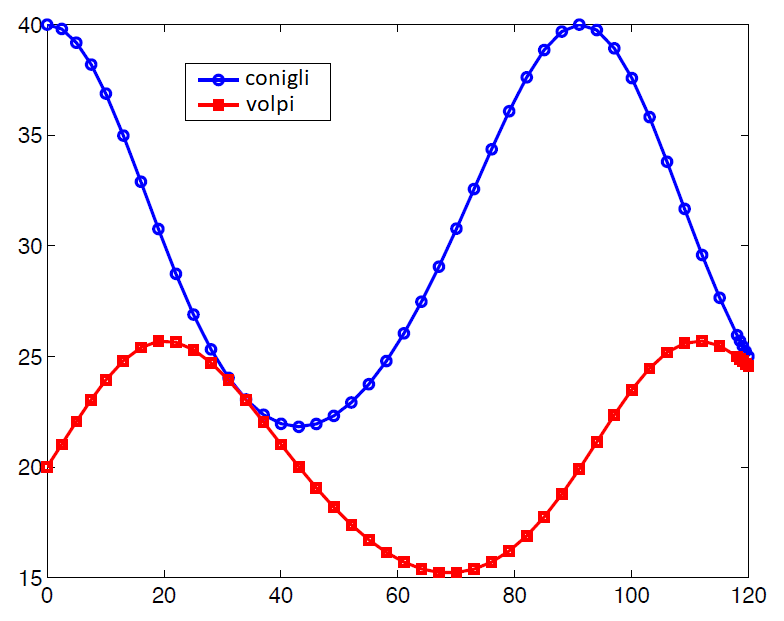
\includegraphics[width=0.62\textwidth]{9ff563ba-c6af-471e-b30a-05ce2fcac5fa.png}
\caption{Esempio di andamento delle due popolazioni nel modello preda-predatore.}
\end{figure}

\section{Il problema di Cauchy}
I precedenti sono esempi di sistemi di equazioni differenziali ordinarie. In particolare, rappresentano esempi del problema di Cauchy, che qui consideriamo del prim'ordine.

Sia $I=[t_0,T]$ l'intervallo temporale di interesse. Il problema di Cauchy generale consiste nel
\[
\text{trovare } y:I\subset\R\to\R^n \text{ tale che }
\begin{cases}
 y'(t)=f(t,y(t)), & \forall t\in I,\\[0.2em]
 y(t_0)=y_0,
\end{cases}
\]

con $f:I\times\R^m\to\R^m$ funzione vettoriale assegnata, in generale non lineare in $y$.

Nel caso scalare ($m=1$) si ottiene il problema di Cauchy scalare:
\[
\text{trovare } y:I\subset\R\to\R \text{ tale che }
\begin{cases}
 y'(t)=f(t,y(t)), & \forall t\in I,\\[0.2em]
 y(t_0)=y_0.
\end{cases}
\]

con $f:I\times\R\to\R$ funzione assegnata.

\subsection{Esistenza e unicit\`a della soluzione continua}
Richiamiamo il seguente risultato.

\begin{proposition}
Supponiamo che la funzione $f(t,y)$ sia:
\begin{enumerate}[label=\arabic*.]
\item limitata e continua rispetto ad entrambi gli argomenti;
\item lipschitziana rispetto al secondo argomento, ossia esista una costante $L>0$ tale che
\[
|f(t,y_1)-f(t,y_2)|\le L|y_1-y_2| \qquad \forall t\in I,\ \forall y_1,y_2\in\R.
\]
\end{enumerate}
Allora la soluzione del problema di Cauchy esiste, \`e unica ed \`e di classe $C^1$ su $I$.
\end{proposition}

\subsection{Esempio}
Sia $I=[0,2]$ e $f(t,y)=3y-3t$. Consideriamo
\[
\begin{cases}
 y'(t)=3y(t)-3t,\\
 y(0)=1.
\end{cases}
\]
In questo caso
\[
|f(t,y_1)-f(t,y_2)|=|3y_1-3t-(3y_2-3t)|=3|y_1-y_2|,
\]
quindi la soluzione esiste unica. Essa \`e data da
\[
 y(t)=\frac{2}{3}e^{3t}+t+\frac13.
\]

\begin{figure}[H]
\centering
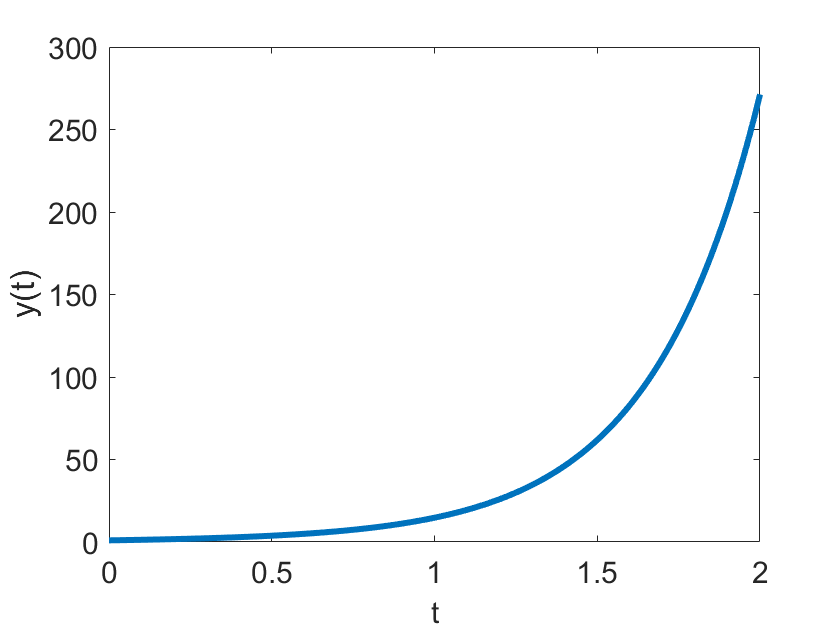
\includegraphics[width=0.5\textwidth]{40a23c9c-ae70-4423-9315-efb181c492f6.png}
\caption{Andamento della soluzione dell'esempio scalare $y'(t)=3y(t)-3t$.}
\end{figure}

\section{Approssimazione di derivate}
Al fine di approssimare il problema di Cauchy, affrontiamo prima il seguente problema: siano noti i valori $v(t_n)$ di una funzione $v$ in corrispondenza di nodi temporali $t_n$, $n=0,\dots,N$, e si vogliano approssimare i valori della sua derivata prima $v'(t)$ negli stessi nodi.

Introduciamo nodi equispaziati
\[
 t_n=t_0+nh, \qquad n=0,\dots,N, \qquad h=\frac{T-t_0}{N}.
\]

\begin{figure}[H]
\centering
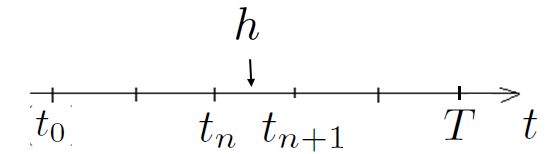
\includegraphics[width=0.42\textwidth]{ch5_time_grid_final.png}
\caption{Griglia temporale equispaziata.}
\end{figure}

Dallo sviluppo in serie di Taylor abbiamo
\begin{equation}\label{eq:taylor-forward}
 v(t_{n+1})=v(t_n)+hv'(t_n)+\frac{h^2}{2}v''(t_n)+\frac{h^3}{6}v'''(t_n)+O(h^4).
\end{equation}
Si ricorda che una quantit\`a \`e un $O(h^p)$ se vale
\[
 \lim_{h\to 0}\frac{O(h^p)}{h^p}<+\infty,
\]
cio\`e se va a $0$ con la stessa velocit\`a o pi\`u velocemente di $h^p$.

Dalla precedente possiamo scrivere
\[
 v'(t_n)=\frac{v(t_{n+1})-v(t_n)}{h}-\frac{h}{2}v''(t_n)-\frac{h^2}{6}v'''(t_n)+O(h^3).
\]
Ci\`o permette di introdurre un'approssimazione in avanti della derivata prima:
\[
 D^+v(t_n)=\frac{v(t_{n+1})-v(t_n)}{h}
\]

il cui errore \`e dato da
\begin{equation}\label{eq:forward-accuracy}
 |v'(t_n)-D^+v(t_n)|=O(h).
\end{equation}

Partendo invece dallo sviluppo di Taylor all'indietro
\begin{equation}\label{eq:taylor-backward}
 v(t_{n-1})=v(t_n)-hv'(t_n)+\frac{h^2}{2}v''(t_n)-\frac{h^3}{6}v'''(t_n)+O(h^4),
\end{equation}
otteniamo, con passaggi analoghi, l'approssimazione all'indietro della derivata prima:
\[
 D^-v(t_n)=\frac{v(t_n)-v(t_{n-1})}{h}
\]

il cui errore \`e ancora dato da
\begin{equation}\label{eq:backward-accuracy}
 |v'(t_n)-D^-v(t_n)|=O(h).
\end{equation}

Per completezza riportiamo anche l'approssimazione centrata
\[
 D^cv(t_n)=\frac{v(t_{n+1})-v(t_{n-1})}{2h}
\]

Questa approssimazione non verr\`a utilizzata in seguito. Sottraendo \eqref{eq:taylor-backward} da \eqref{eq:taylor-forward} si ottiene il contenuto del box rosso dei lucidi.

% [BOX ROSSO NEI LUCIDI -- NON RICHIESTO ALL'ESAME]
\begin{nonExamBox}
\[
 v(t_{n+1})-v(t_{n-1})=2hv'(t_n)+\frac{h^3}{3}v'''(t_n)+O(h^4),
\]
cio\`e
\[
 \frac{v(t_{n+1})-v(t_{n-1})}{2h}=v'(t_n)+\frac{h^2}{6}v'''(t_n)+O(h^3).
\]
\end{nonExamBox}
Quindi
\[
 |v'(t_n)-D^cv(t_n)|=O(h^2),
\]
ossia si tratta di un metodo di ordine $2$.

\begin{figure}[H]
\centering
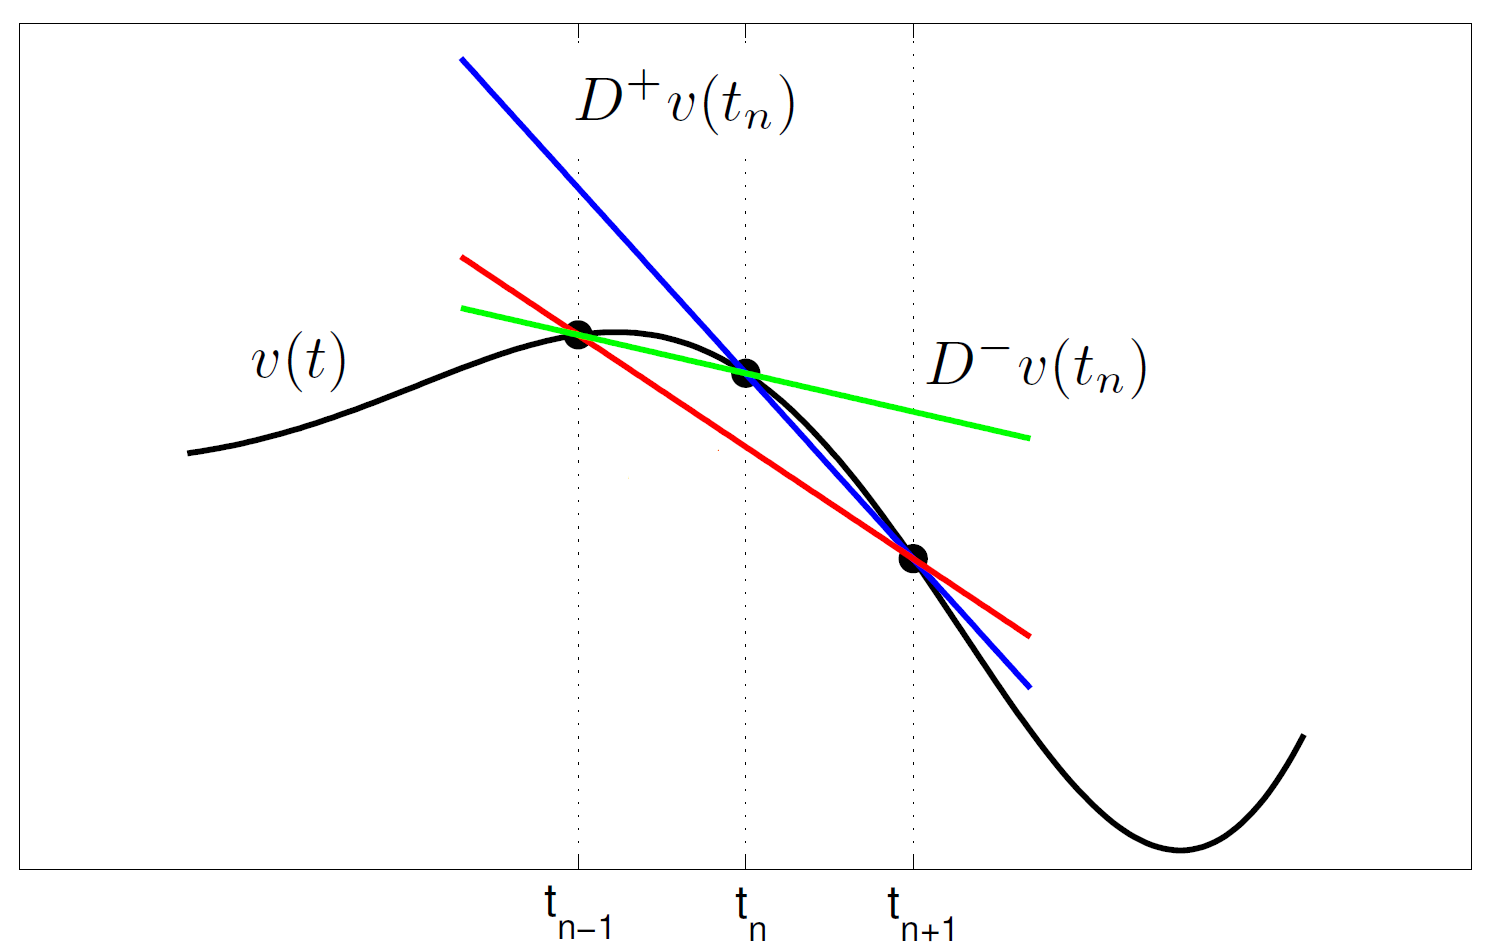
\includegraphics[width=0.56\textwidth]{2b3b1a21-cdae-458f-a081-d4892ef32b6d.png}
\caption{Approssimazioni in avanti (blu) e all'indietro (verde) della derivata prima; in rosso l'approssimazione centrata.}
\end{figure}

\section{Approssimazione numerica del problema di Cauchy}
In generale non \`e possibile risolvere analiticamente il problema di Cauchy. Servono quindi metodi numerici per approssimarlo.

Tali metodi permettono di determinare una soluzione numerica
\[
 u_n,\qquad n=0,\dots,N,\qquad N=\frac{T}{h},
\]
con $u_0=y_0$. Il metodo numerico deve produrre una soluzione $u_n$ che sia una buona approssimazione di $y(t_n)$ per ogni $n$.

In generale si considerano i seguenti passi:
\begin{enumerate}[label=\arabic*)]
\item si suddivide l'intervallo temporale in nodi $t_n$;
\item si scrive, per ogni $n=1,\dots,N=T/h$, il problema di Cauchy per il generico nodo $t_n$;
\item si sostituisce, per ogni $n$, a $y'(t_n)$ una delle approssimazioni di prima (ad esempio $D^+y(t_n)$ o $D^-y(t_n)$);
\item si denota, per ogni $n$, con $u_n$ la soluzione del nuovo problema approssimato ottenuto.
\end{enumerate}
Quindi la soluzione approssimata \`e
\[
 \{u_0=y_0,u_1,u_2,\dots,u_N\}.
\]

\section{I metodi di Eulero in avanti e all'indietro}
\subsection{Metodo di Eulero in avanti}
Partiamo dal problema di Cauchy. Esso vale per ogni $t\in I$, quindi in particolare anche in $t_n$:
\[
 y'(t_n)=f(t_n,y(t_n)).
\]
Approssimiamo ora la derivata a sinistra con la sua approssimazione in avanti:
\[
 D^+y(t_n)=\frac{y(t_{n+1})-y(t_n)}{h}\simeq f(t_n,y(t_n)).
\]
Introduciamo allora come soluzione numerica $u_n$, $n=1,\dots,N$, la successione di valori che risolve in maniera esatta la precedente relazione. Questo d\`a luogo al metodo di Eulero in avanti:
\begin{formulaBox}
\[
 u_{n+1}=u_n+h f(t_n,u_n),
 \qquad n=0,\dots,N-1.
\]
\end{formulaBox}

\subsection{Metodo di Eulero all'indietro}
In maniera analoga, partendo per comodit\`a da
\[
 y'(t_{n+1})=f(t_{n+1},y(t_{n+1})),
\]
approssimiamo la derivata a sinistra con la sua approssimazione all'indietro:
\[
 D^-y(t_{n+1})=\frac{y(t_{n+1})-y(t_n)}{h}\simeq f(t_{n+1},y(t_{n+1})).
\]
Introduciamo nuovamente come soluzione numerica $u_n$ la successione che risolve in maniera esatta la precedente relazione. Otteniamo cos\`i il metodo di Eulero all'indietro:
\begin{formulaBox}
\[
 u_{n+1}=u_n+h f(t_{n+1},u_{n+1}),
 \qquad n=0,\dots,N-1.
\]
\end{formulaBox}

Per entrambi i metodi si conosce la condizione iniziale $u_0=y_0$, e ci\`o permette di calcolare in sequenza prima $u_1$, poi $u_2$ e cos\`i via. Non si tratta per\`o di metodi iterativi nel senso dei sistemi lineari: qui la soluzione \`e significativa per ogni $n$, essendo l'approssimazione della soluzione a diversi istanti temporali.

\begin{figure}[H]
\centering
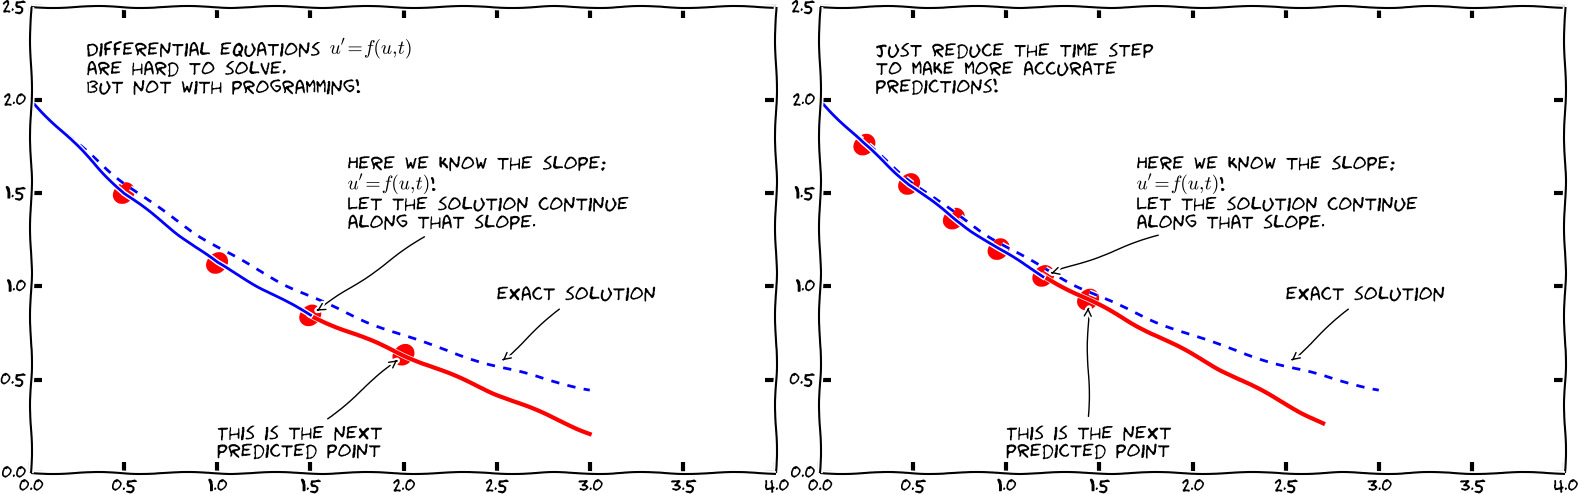
\includegraphics[width=0.9\textwidth]{81343e44-40b8-4797-9711-e2b659992d7b.png}
\caption{Rappresentazione grafica dell'idea dei metodi di Eulero.}
\end{figure}

\subsection{Aspetti computazionali}
Per il metodo di Eulero in avanti il nuovo valore \`e calcolato in maniera esplicita: \`e sufficiente valutare la funzione $f$ nel punto $(t_n,u_n)$. Per questo motivo tale metodo \`e anche detto \emph{metodo di Eulero esplicito}.

Si consideri ad esempio il problema di Cauchy
\[
\begin{cases}
 y'(t)=\arctan(3y(t))-3y(t)+t,\qquad t>1,\\
 y(1)=1.
\end{cases}
\]
Il metodo di Eulero in avanti diventa: dato $u_0=1$, per ogni $n>0$ calcola
\[
 u_{n+1}=u_n+h\bigl(\arctan(3u_n)-3u_n+t_n\bigr).
\]

Invece, per il metodo di Eulero all'indietro,
\[
 u_{n+1}=u_n+h f(t_{n+1},u_{n+1})
\]
non si ha in generale un'espressione esplicita per il nuovo valore $u_{n+1}$, perch\'e esso compare anche a destra dell'uguale. Poniamo $x=u_{n+1}$ la nostra incognita; se $f$ \`e non lineare rispetto a $y$, si deve ad ogni passo temporale risolvere il problema di ricerca degli zeri della funzione
\[
 g(x)=x-u_n-hf(t_{n+1},x).
\]
Se $g(x)$ \`e derivabile, si possono introdurre ad esempio le iterazioni di Newton, per $k\ge 0$,
\[
 x^{(k+1)}=x^{(k)}-\frac{g(x^{(k)})}{g'(x^{(k)})},
\qquad x^{(0)}=u_n.
\]
Nel caso scalare si ottiene
\[
 x^{(k+1)}=x^{(k)}-\frac{x^{(k)}-u_n-hf(t_{n+1},x^{(k)})}{1-hf'(t_{n+1},x^{(k)})}.
\]
Se il metodo di Newton converge,
\[
 \lim_{k\to\infty}x^{(k)}=u_{n+1}.
\]
A causa del fatto che $u_{n+1}$ non pu\`o in generale essere determinato per via esplicita, tale metodo prende anche il nome di \emph{metodo di Eulero implicito}.

Alternativamente, partendo dallo schema implicito, si pu\`o pensare di determinare $u_{n+1}$ risolvendo un problema di punto fisso. In generale possiamo distinguere i metodi numerici per equazioni differenziali ordinarie in metodi \emph{espliciti}, la cui soluzione al nuovo passo temporale \`e calcolata mediante un'espressione esplicita, e metodi \emph{impliciti}, che invece richiedono la soluzione di un'equazione non lineare.

\subsection{Confronto su un esempio}
Riprendiamo il problema di Cauchy dell'esempio precedente. Il metodo di Eulero all'indietro porta, dato $u_0=1$, alla relazione
\[
 u_{n+1}=u_n+h\bigl(\arctan(3u_{n+1})-3u_{n+1}+t_{n+1}\bigr),
\]
che porta ad ogni passo $n$ alla ricerca della radice della funzione non lineare
\[
 g(x)=x-u_n-h\bigl(\arctan(3x)-3x+t_{n+1}\bigr).
\]
A parit\`a di passo $h$ i due metodi di Eulero producono due diverse approssimazioni; nell'esempio dei lucidi, con $h=0.4$, entrambe appaiono accurate.


\section{Assoluta stabilit\`a}
Vogliamo discutere quando la soluzione numerica fornita dai metodi di Eulero sia esente da oscillazioni che aumentano indefinitamente, producendo una soluzione non stabile e quindi non accettabile. Il concetto rigoroso introdotto a questo fine \`e quello di \emph{assoluta stabilit\`a}.

A tal fine si considerano le prestazioni numeriche dei vari metodi quando applicati al problema modello lineare
\[
 y'(t)=\lambda y(t),
\qquad \lambda<0,
\]
la cui soluzione esatta \`e
\[
 y(t)=y_0e^{\lambda(t-t_0)}.
\]
Dato $h>0$, il metodo numerico si dice assolutamente stabile per quel valore di $h$ se
\[
 \lim_{n\to\infty}u_n=0,
\]
oppure, equivalentemente, se su un intervallo illimitato si ha $|u_n|\to 0$ per $n\to\infty$.

\subsection{Analisi dell'assoluta stabilit\`a per Eulero in avanti}
Applicando il metodo di Eulero in avanti al problema modello otteniamo
\[
 u_{n+1}=u_n+h\lambda u_n=(1+h\lambda)u_n,
\]
quindi
\[
 u_n=(1+h\lambda)^n u_0.
\]
L'assoluta stabilit\`a \`e garantita se
\[
 |1+h\lambda|<1,
\]
cio\`e per
\begin{formulaBox}
\[
 -2<h\lambda<0.
\]
\end{formulaBox}
Se $\lambda<0$, questo equivale a richiedere $h$ sufficientemente piccolo.

\subsection{Esempi}
Consideriamo il problema
\[
 y'(t)=-2y(t), \qquad y(0)=1.
\]
La soluzione esatta \`e $y(t)=e^{-2t}$.

Con Eulero in avanti e $h=1.1$ si ottiene
\[
 u_{n+1}=(1-2h)u_n=-1.2\,u_n,
\]
da cui si evince che la soluzione numerica \`e oscillante ed esplode. Con $h=0.2$ si ha invece
\[
 u_{n+1}=0.6\,u_n,
\]
e la soluzione numerica non oscilla e diminuisce per $n$ crescente, come la soluzione esatta. Procedendo analogamente, si troverebbe che:
\begin{itemize}
\item per $h=1.0$ la soluzione \`e oscillante ma con modulo costante;
\item per $h=0.9$ la soluzione \`e oscillante ma diminuisce per $n$ crescente.
\end{itemize}
Dall'esempio si evince che:
\begin{itemize}
\item per $h$ troppo grande la soluzione numerica oscilla ed esplode;
\item per $h$ intermedi la soluzione numerica oscilla ma non esplode;
\item per $h$ piccolo la soluzione numerica non oscilla.
\end{itemize}

\begin{figure}[H]
\centering
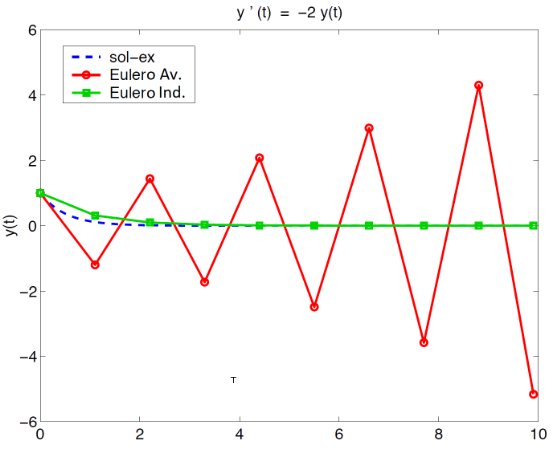
\includegraphics[width=0.65\textwidth]{178c7f03-9ed3-46bf-b8b4-5ec4546d9500.png}
\caption{Soluzione esatta e soluzioni numeriche con Eulero in avanti per $h=0.9$ e $h=1.1$.}
\end{figure}

\begin{figure}[H]
\centering
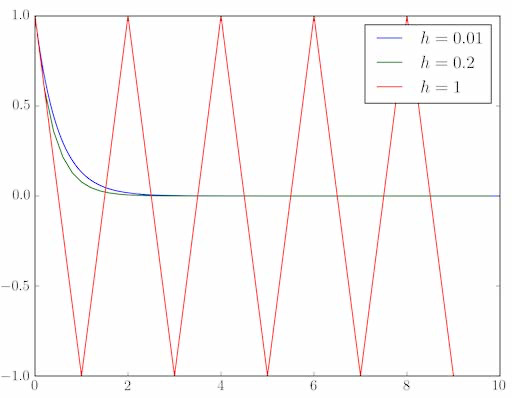
\includegraphics[width=0.62\textwidth]{3245c4e6-fd4b-4721-876c-a55260b20b07.png}
\caption{Esempio di assoluta stabilit\`a di Eulero in avanti al variare del passo $h$.}
\end{figure}

\subsection{Assoluta stabilit\`a di Eulero all'indietro}
Applicando il metodo di Eulero all'indietro al problema modello si ottiene
\[
 u_{n+1}=u_n+h\lambda u_{n+1},
\]
quindi
\[
 u_{n+1}=\frac{1}{1-h\lambda}u_n,
\qquad
 u_n=\left(\frac{1}{1-h\lambda}\right)^n u_0.
\]
In questo caso l'assoluta stabilit\`a \`e sempre garantita, infatti per $\lambda<0$ e $h>0$ si ha
\[
 \left|\frac{1}{1-h\lambda}\right|<1.
\]
Quindi il metodo di Eulero all'indietro \`e \emph{incondizionatamente assolutamente stabile}.

\begin{figure}[H]
\centering
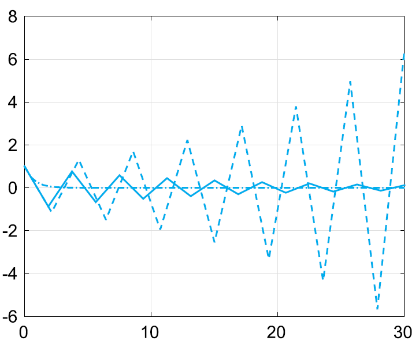
\includegraphics[width=0.62\textwidth]{4c9368e4-08ee-4efb-906d-7003db0048a2.png}
\caption{Soluzione esatta e soluzioni numeriche con Eulero in avanti ed Eulero all'indietro per $h=1.1$.}
\end{figure}

\begin{figure}[H]
\centering
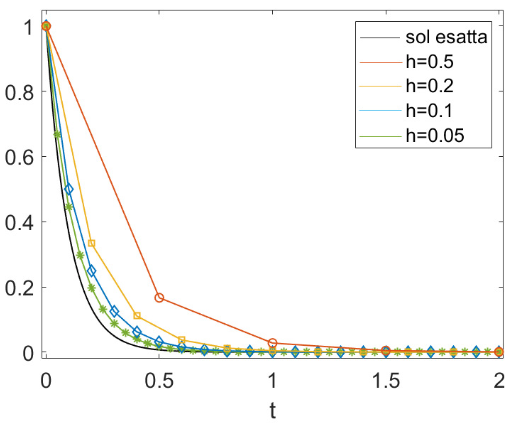
\includegraphics[width=0.58\textwidth]{faa0d3ff-b458-46b6-afb3-26e867684981.png}
\caption{Soluzione ottenuta con Eulero all'indietro del problema $y'(t)=-2y(t)$ per diversi valori di $h$. La soluzione \`e sempre stabile, ma con $h$ grande si perde in accuratezza.}
\end{figure}

\subsection{Problemi generali}
Diremo che un metodo numerico produce una soluzione stabile se a ``piccole'' perturbazioni sul dato iniziale si producono perturbazioni ``piccole'' e decrescenti per $n$ crescente.

Notando che per il problema modello si ha
\[
 \frac{\partial f}{\partial y}=\lambda,
\]
ha senso introdurre la seguente stima cautelativa dell'intervallo dei valori di $h$ che garantiscono una soluzione stabile per il metodo di Eulero in avanti:
\begin{formulaBox}
\[
 h<\frac{2}{\displaystyle \max_{(t,y)}\left|\frac{\partial f}{\partial y}(t,y)\right|}.
\]
\end{formulaBox}
In generale, vale la propriet\`a che un metodo numerico assolutamente stabile per il problema modello sotto una condizione su $h$ produce una soluzione numerica stabile anche per il problema di Cauchy generico sotto la stessa condizione opportunamente adattata.

\begin{figure}[H]
\centering
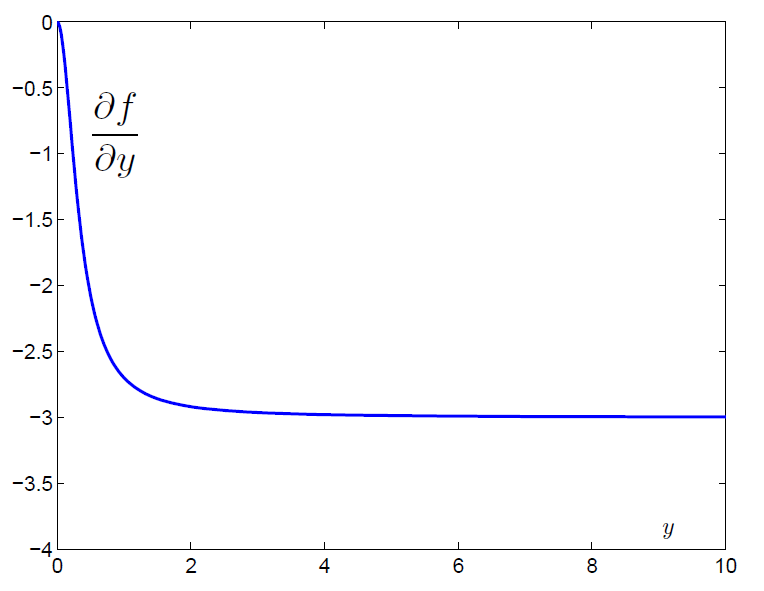
\includegraphics[width=0.42\textwidth]{bf2d96f5-4e2b-434f-a89e-86c167e52942.png}
\caption{Andamento di $\dfrac{\partial f}{\partial y}$ nell'esempio 4-ter.}
\end{figure}

Nell'esempio 4-ter dei lucidi si ottiene
\[
 h<\frac{2}{3}.
\]
Pertanto il metodo di Eulero in avanti \`e stabile se $h<2/3$.

\begin{figure}[H]
\centering
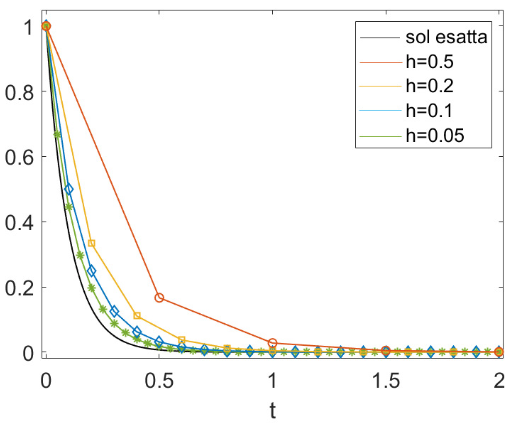
\includegraphics[width=0.76\textwidth]{faa0d3ff-b458-46b6-afb3-26e867684981.png}
\caption{Soluzione esatta e approssimazioni ottenute con Eulero in avanti per diversi passi temporali che soddisfano la condizione di stabilit\`a.}
\end{figure}

\section{Il metodo di Crank--Nicolson}
Partiamo dal problema di Cauchy
\[
 y'(t)=f(t,y(t)), \qquad y(t_0)=y_0.
\]
Dal teorema fondamentale del calcolo integrale limitato all'intervallo $[t_n,t_{n+1}]$ otteniamo
\[
 y(t_{n+1})=y(t_n)+\int_{t_n}^{t_{n+1}} f(t,y(t))\,dt.
\]
Possiamo adesso applicare una formula di quadratura per approssimare l'integrale a destra dell'uguale. Usando la formula dei trapezi su un solo intervallo si ottiene
\[
 \int_{t_n}^{t_{n+1}} f(t,y(t))\,dt \simeq \frac{h}{2}\bigl(f(t_n,y(t_n))+f(t_{n+1},y(t_{n+1}))\bigr).
\]
Introducendo la soluzione numerica $u_n$, si ottiene il metodo di Crank--Nicolson:
\begin{formulaBox}
\[
 u_{n+1}=u_n+\frac{h}{2}\Bigl(f(t_n,u_n)+f(t_{n+1},u_{n+1})\Bigr).
\]
\end{formulaBox}
Il metodo di Crank--Nicolson \`e implicito e richiede ad ogni passo $n$ di determinare la radice di un'equazione non lineare.

Riguardo all'assoluta stabilit\`a, considerando il problema modello $y'(t)=\lambda y(t)$ si ha
\[
 u_{n+1}=u_n+\frac{h}{2}\lambda(u_n+u_{n+1}),
\]
cio\`e
\[
 u_{n+1}=\frac{1+\frac{h\lambda}{2}}{1-\frac{h\lambda}{2}}u_n.
\]
Perci\`o
\[
 \left|\frac{1+\frac{h\lambda}{2}}{1-\frac{h\lambda}{2}}\right|<1,
\]
per ogni $h>0$ e $\lambda<0$. Segue che CN, come EI, \`e incondizionatamente assolutamente stabile.



\begin{figure}[H]
\centering
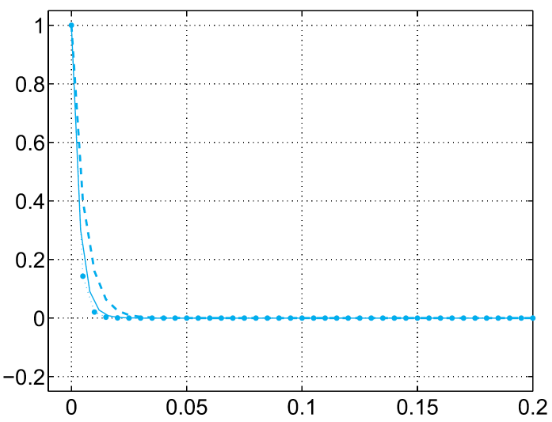
\includegraphics[width=0.55\textwidth]{Screenshot from 2026-03-30 00-33-25.png}
\caption{Maggior accuratezza di Crank--Nicolson (pallini) rispetto a Eulero in avanti (tratteggio) a parit\`a di passo $h$. In linea continua la soluzione esatta.}
\end{figure}

\section{Il metodo di Heun}
Partiamo dal metodo di Crank--Nicolson. Se al posto di $u_{n+1}$ a destra introduciamo la sua approssimazione ottenuta con il metodo di Eulero in avanti, otteniamo il metodo di Heun:
\begin{formulaBox}
\[
 u_{n+1}=u_n+\frac{h}{2}\Bigl[f(t_n,u_n)+f\bigl(t_{n+1},u_n+h f(t_n,u_n)\bigr)\Bigr].
\]
\end{formulaBox}
Esso \`e un metodo esplicito grazie alla sostituzione fatta, con condizione di assoluta stabilit\`a uguale a quella di EA.

\section{Convergenza}
Abbiamo discusso quando un metodo numerico produce una soluzione stabile. Abbiamo trovato che ci\`o in generale avviene per $h$ sufficientemente piccolo. Ci chiediamo ora quale sia l'accuratezza della soluzione numerica per tali valori di $h$.

Introduciamo la definizione di convergenza. Un metodo numerico si dice convergente se, per ogni nodo fissato $t_n$,
\[
 \lim_{h\to 0}|y(t_n)-u_n|=0.
\]
Se in particolare vale che
\begin{formulaBox}
\[
 |y(t_n)-u_n|\le Ch^p,
\]
\end{formulaBox}
allora diremo che il metodo numerico \`e di ordine $p$. Pi\`u $p$ \`e grande, pi\`u il metodo converger\`a velocemente.

\begin{figure}[H]
\centering
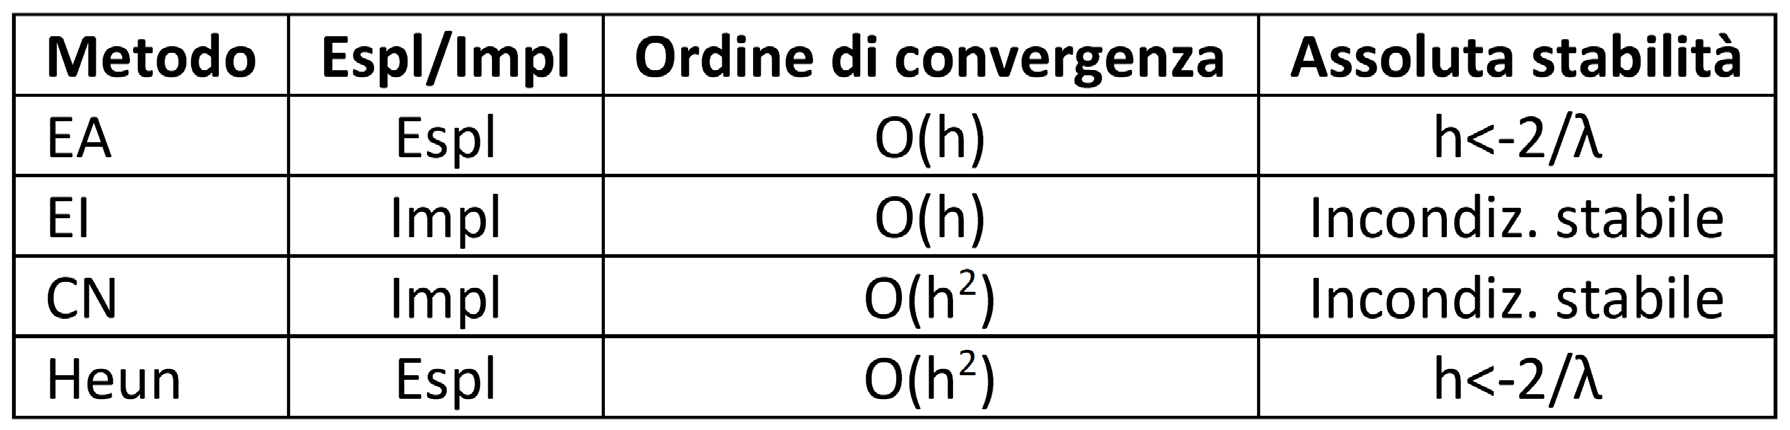
\includegraphics[width=0.92\textwidth]{62664e10-350b-423d-8917-b90753c4eb2c.png}
\caption{Propriet\`a di convergenza e assoluta stabilit\`a dei metodi visti.}
\end{figure}

\subsection{Consistenza}
I metodi di Eulero sono stati costruiti a partire da formule accurate del prim'ordine per l'approssimazione di derivate. Introduciamo l'errore di troncamento locale: questo \`e l'errore che si commette introducendo la soluzione esatta $y$ nello schema numerico.

Per il metodo di Eulero in avanti abbiamo
\[
 \tau_n^{EA}=\frac{y(t_{n+1})-y(t_n)}{h}-f(t_n,y(t_n)).
\]
Diremo che un metodo numerico \`e consistente se vale
\[
 \lim_{h\to 0}\tau_n=0.
\]
Se in particolare vale
\[
 |\tau_n|\le Ch^p,
\]
diremo che l'ordine di consistenza \`e $p$.

Ricordando che $y'=f$, per il metodo EA vale
\[
 \tau_n^{EA}=\frac{y(t_{n+1})-y(t_n)}{h}-y'(t_n)=O(h),
\]
dove nell'ultima uguaglianza si \`e usato il risultato di accuratezza \eqref{eq:forward-accuracy} dell'approssimazione in avanti della derivata prima. Analogamente, per il metodo di Eulero all'indietro
\[
 \tau_n^{EI}=\frac{y(t_n)-y(t_{n-1})}{h}-y'(t_n)=O(h),
\]
avendo utilizzato il risultato di accuratezza \eqref{eq:backward-accuracy}. I metodi di Eulero sono quindi consistenti del prim'ordine.

\subsection{Errore globale e convergenza di Eulero in avanti}
\`E importante far notare che l'errore di troncamento locale non \`e l'errore di convergenza. L'errore globale
\[
 e_n=y(t_n)-u_n
\]
\`e infatti dato da due contributi:
\begin{itemize}
\item l'errore $e_n^{(1)}$ dovuto localmente al metodo numerico, ottenuto partendo dalla vera soluzione $y(t_{n-1})$;
\item l'errore $e_n^{(2)}$ dovuto alla propagazione degli errori commessi agli istanti precedenti.
\end{itemize}

\begin{figure}[H]
\centering
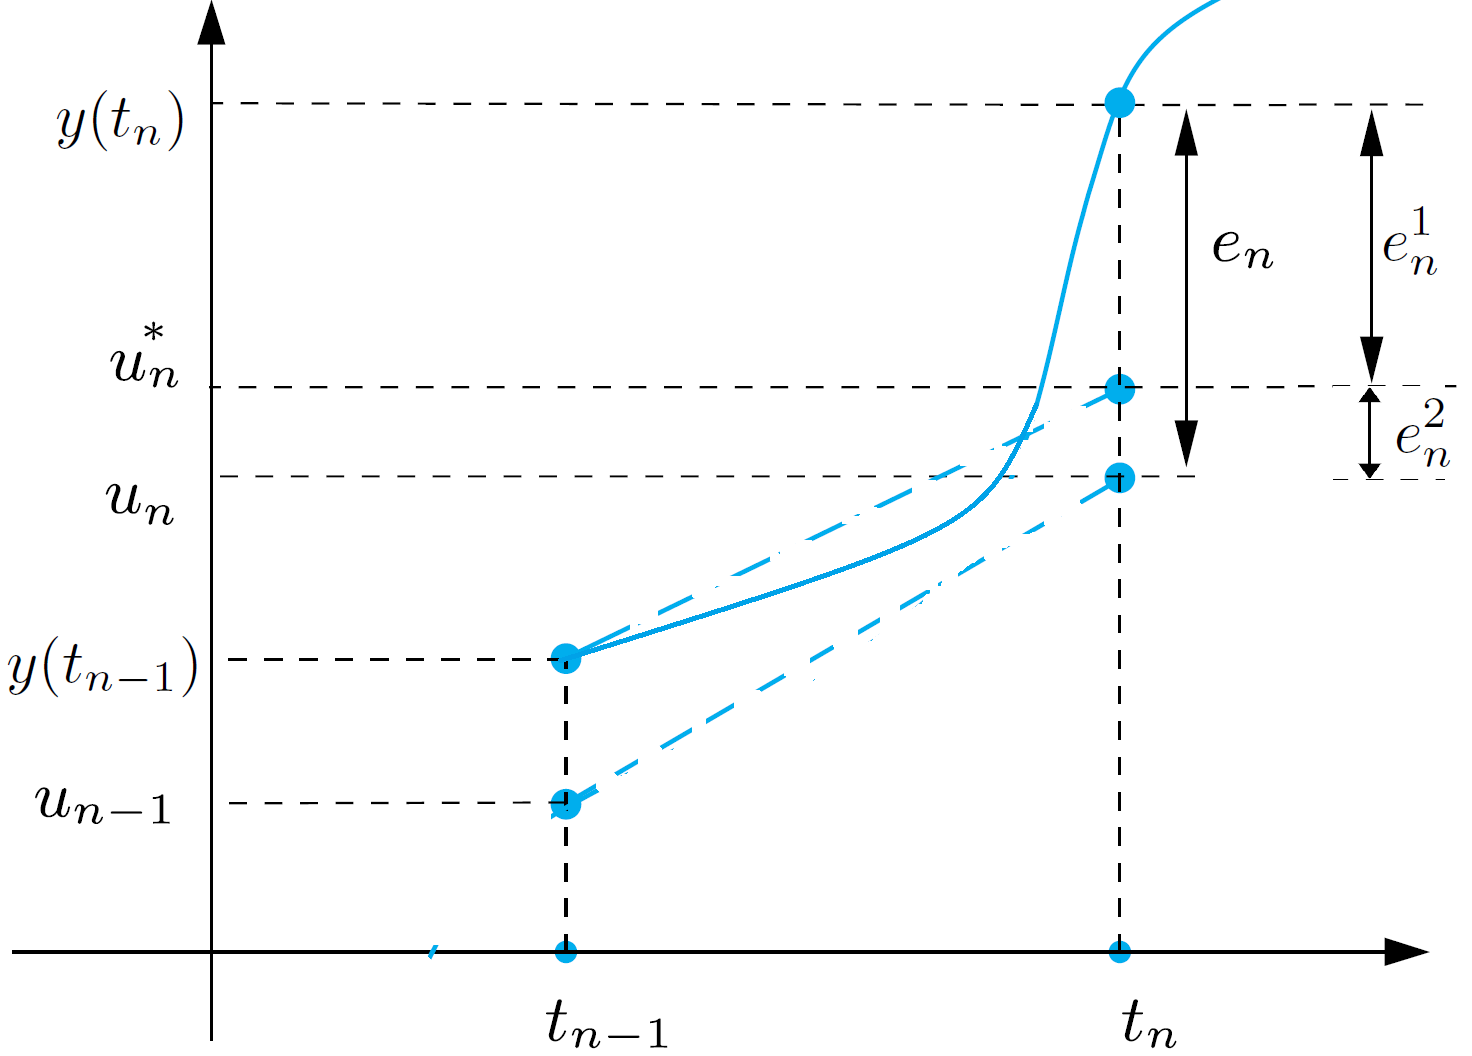
\includegraphics[width=0.82\textwidth]{c2609531-5d94-4c64-a465-2bde67423ecf.png}
\caption{Scomposizione dell'errore globale nel contributo locale $e_n^{(1)}$ e nel contributo di propagazione $e_n^{(2)}$.}
\end{figure}

Indicando con $\tilde u_n$ la soluzione che il metodo di EA produrrebbe partendo dalla soluzione esatta $y(t_{n-1})$, si ottiene
\[
 e_n=e_n^{(1)}+e_n^{(2)}.
\]
Il primo contributo \`e, a meno di un fattore $h$, dato dall'errore di troncamento locale. Questo evidenzia come la consistenza da sola non basti per avere la convergenza: serve qualche altra propriet\`a che controlli la produzione degli errori agli istanti precedenti e la loro conseguente propagazione.

Riguardo al secondo contributo, supponiamo che $f$ sia continua e che esista $L$ tale che
\[
 |f(t,y_1)-f(t,y_2)|\le L|y_1-y_2|.
\]
Allora, per il teorema del valor medio, esiste $\xi_n$ compreso fra $y(t_n)$ e $u_n$ tale che
\[
 |e_{n+1}|\le (1+hL)|e_n|+Ch^2.
\]
Supponiamo ora che valga la condizione di assoluta stabilit\`a per Eulero in avanti con $\lambda=-L$:
\[
 h<\frac{2}{L}.
\]
Allora, usando ricorsivamente la disuguaglianza precedente e notando che $e_0=0$, si ottiene
\[
 |e_n|\le Ch,
\]
con costante indipendente da $h$. Il metodo di Eulero in avanti \`e dunque convergente e del prim'ordine.

In generale, possiamo affermare che, per un metodo convergente, l'ordine di convergenza \`e uguale all'ordine di consistenza. Si pu\`o mostrare che anche il metodo di Eulero all'indietro \`e convergente e del prim'ordine.

\begin{figure}[H]
\centering
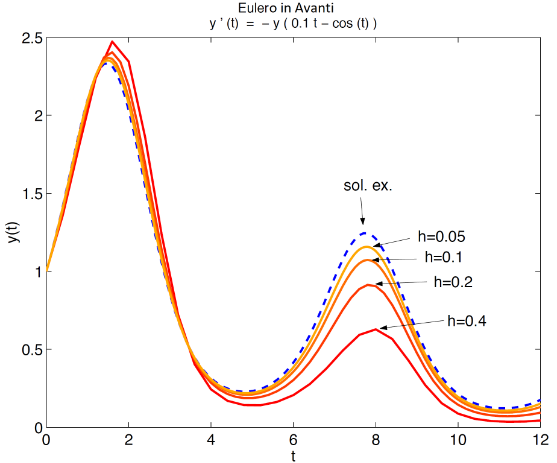
\includegraphics[width=0.66\textwidth]{Screenshot from 2026-03-30 00-34-06.png}
\caption{Esempio finale: soluzione numerica ottenuta con Eulero in avanti per diversi valori del passo $h$, confrontata con la soluzione esatta.}
\end{figure}

\subsection{Assoluta stabilit\`a e convergenza}
Il concetto di assoluta stabilit\`a di un metodo numerico \`e legato al valore di $h$ finito che si sta considerando. Lo stesso metodo numerico pu\`o essere assolutamente stabile per alcuni valori di $h$ e non assolutamente stabile per altri valori di $h$. L'assoluta stabilit\`a analizza il comportamento della soluzione numerica per $h$ fissato e al crescere di $n$. La convergenza \`e invece una propriet\`a dell'errore per $n$ fissato e facendo tendere $h$ a $0$.

Un metodo consistente ma usato per valori di $h$ che violino la condizione di stabilit\`a produrr\`a delle soluzioni numeriche instabili, dunque non significative.

\begin{figure}[H]
\centering
\begin{minipage}[t]{0.47\textwidth}
\centering
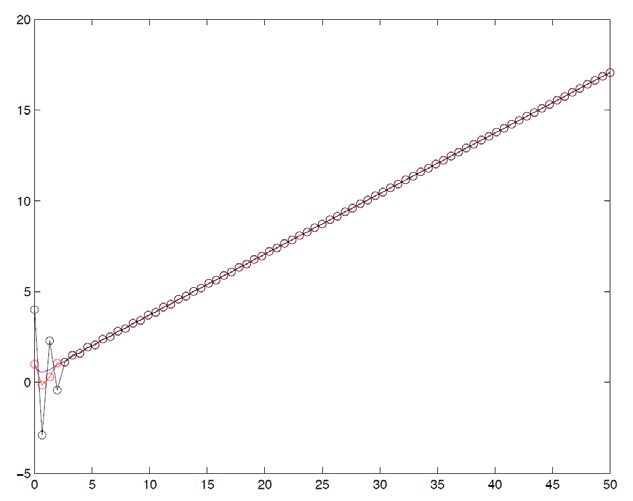
\includegraphics[width=\linewidth]{68274b40-b174-490a-b61f-ae0fa208366c.png}
\end{minipage}\hfill
\begin{minipage}[t]{0.47\textwidth}
\centering
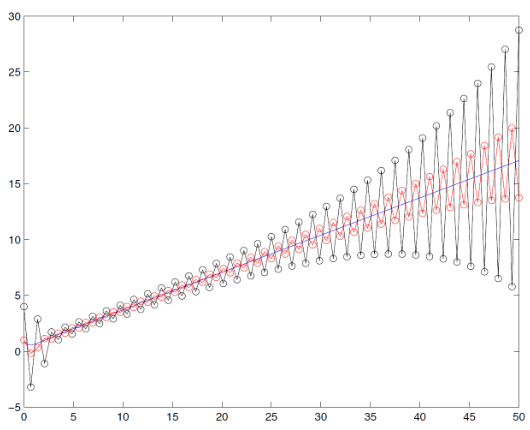
\includegraphics[width=\linewidth]{9aa6297c-1a09-4a5a-816a-45ad5224b9d7.png}
\end{minipage}
\caption{Soluzione numerica in rosso e soluzione numerica del problema perturbato in nero/grigio: a sinistra un caso stabile, a destra un caso non stabile.}
\end{figure}

\begin{noteBox}
Come discusso nei lucidi, il metodo di Eulero in avanti ha il vantaggio di avere costi computazionali ridotti per il calcolo della soluzione corrente, ma ha limitate propriet\`a di assoluta stabilit\`a che richiedono $h$ piccolo. D'altro canto, Eulero all'indietro e Crank--Nicolson hanno migliori propriet\`a di stabilit\`a, ma richiedono la soluzione di un problema implicito ad ogni passo temporale.
\end{noteBox}


\end{document}
